\documentclass[a4paper, 12pt, fleqn]{article}

% \usepackage[utf8]{inputenc}
% \usepackage{tgtermes}
% \usepackage{fouriernc}
\usepackage[T1]{fontenc}
\usepackage[margin=3cm]{geometry}
\usepackage[english]{babel}
\usepackage{microtype}

\usepackage{biblatex}
\addbibresource{refs.bib}

\usepackage{amssymb}
\usepackage{amsmath}

\usepackage{caption}
\usepackage{subcaption}

\usepackage{ebproof}

\usepackage{enumerate}
\usepackage{verbatim}

\usepackage{xcolor}

\usepackage{listings}
\lstset{mathescape=true,
 xleftmargin=.25in}
\usepackage{quiver}

\usepackage[ruled]{algorithm2e}
\SetKwInput{Input}{\sc Input}
\SetKwInput{Output}{\sc Output}
\SetKwComment{Comment}{/*}{*/}

\usepackage[skip=10pt]{parskip}

\newcommand{\N}{\mathbb{N}}
\newcommand{\Z}{\mathbb{Z}}
\newcommand{\Q}{\mathbb{Q}}
\newcommand{\R}{\mathbb{R}}
\newcommand{\C}{\mathbb{C}}
\newcommand{\B}{\mathbb{B}}
\newcommand{\dif}{\mathrm{d}}
\DeclareMathOperator{\Arg}{Arg}
\DeclareMathOperator{\IN}{IN}
\DeclareMathOperator{\LT}{lt}
\DeclareMathOperator{\LM}{lm}
\DeclareMathOperator{\LC}{lc}
\DeclareMathOperator{\coef}{coef}
\DeclareMathOperator{\lcm}{lcm}
\DeclareMathOperator{\Spec}{Spec}
\DeclareMathOperator{\V}{\mathbf V}
\DeclareMathOperator{\I}{\mathbf I}
\DeclareMathOperator{\J}{\mathbf J}
\newcommand{\p}{\mathfrak p}
\newcommand{\fr}[1]{\mathfrak{#1}}
\newcommand{\la}[1]{\lambda{#1}.\,}


% Kan Danny godt lide
\usepackage[autostyle]{csquotes}
% \usepackage{kpfonts}
% \usepackage{inconsolata}
\linespread{1.06}


% \usepackage{minted}
% \usemintedstyle{tango}
% \setminted{fontsize=\footnotesize}
% \setminted{breaklines}
% \newcommand{\lean}[1]{\mintinline{lean}{#1}}

\usepackage{fontspec}
% \setmonofont{JuliaMono}
% \setmainfont{Linux Libertine O}
% \setmathfont[Digits, Latin]{Linux Biolinum O}
\usepackage{libertinus}
% \usepackage{ebgaramond-maths}
% \usepackage{ebgaramond}
% \usepackage[cmintegrals, cmbraces]{newtxmath}

\usepackage{xcolor}
\usepackage{hyperref}
\hypersetup{%
	pdftitle=Parametric Gröbner bases,
	pdfauthor={Andreas Bøgh Poulsen},
	colorlinks,
	linkcolor={red!50!black},
	citecolor={red!50!black},
	urlcolor={red!50!black},
	bookmarksnumbered=true
}

\usepackage[ntheorem]{mdframed}
\usepackage[amsmath,thmmarks,hyperref]{ntheorem}
\usepackage[capitalize]{cleveref}

% \usepackage{thmtools}
% \usepackage{thm-restate}

% Frame for theorems
\definecolor{shadecolor}{gray}{0.93}
\definecolor{rulecolor}{gray}{0.4}
\mdfdefinestyle{thmframed}{%
	%usetwoside=false, % For use with memoir twoside
	skipabove=0.5em plus 0.4em minus 0.2em,
	skipbelow=0.5em plus 0.4em minus 0.2em,
	leftmargin=-7pt, rightmargin=-7pt, innerleftmargin=6pt,
	innerrightmargin=6pt, innertopmargin=6pt, innerbottommargin=3pt,
	% linewidth=1pt, linecolor=rulecolor, backgroundcolor=shadecolor,
  linewidth=1.5pt, linecolor=rulecolor, topline=false, bottomline=false, rightline=false, %leftmargin=1em,
	splittopskip=1.2em minus 0.2em,
	splitbottomskip=0.5em plus 0.2em minus 0.1em,
}
\mdfdefinestyle{thmempty}{
  usetwoside=false, % For use with memoir twoside
	skipabove=0.5em plus 0.4em minus 0.2em,
	skipbelow=0.5em plus 0.4em minus 0.2em,
	leftmargin=-7pt, rightmargin=-7pt, innerleftmargin=6pt,
	innerrightmargin=6pt, innertopmargin=6pt, innerbottommargin=3pt,
	% linewidth=1pt, linecolor=rulecolor, backgroundcolor=shadecolor,
  linewidth=1.5pt, linecolor=rulecolor, topline=false, bottomline=false, rightline=false,
	splittopskip=1.2em minus 0.2em,
	splitbottomskip=0.5em plus 0.2em minus 0.1em,
}

% New theorem style with a dot
\makeatletter
\newtheoremstyle{changedot}%
  {\item[\hskip\labelsep \theorem@headerfont ##2~~$\cdot$~~##1\theorem@separator]}%
  {\item[\hskip\labelsep \theorem@headerfont ##2~~$\cdot$~~##1\ (##3)\theorem@separator]}

\newtheoremstyle{changedotbreak}%
  {\item\hbox to \textwidth{\theorem@headerfont ##2~~$\cdot$~~##1\theorem@separator\hfill}}%
  {\item\hbox to \textwidth{\theorem@headerfont ##2~~$\cdot$~~##1\
      (##3)\theorem@separator\hfill}}
\makeatother

\theoremstyle{changedot}
\theoremseparator{.}
% \newmdtheoremenv[style=thmframed]{theorem}{Theorem}[section]
% \newmdtheoremenv[style=thmframed]{proposition}[theorem]{Proposition}
% \newmdtheoremenv[style=thmframed]{lemma}[theorem]{Lemma}
% \newmdtheoremenv[style=thmframed]{corollary}[theorem]{Corollary}
\newmdtheoremenv[style=thmempty]{theorem}{Theorem}[section]
\newmdtheoremenv[style=thmempty]{proposition}[theorem]{Proposition}
\newmdtheoremenv[style=thmempty]{lemma}[theorem]{Lemma}
\newmdtheoremenv[style=thmempty]{corollary}[theorem]{Corollary}
\newmdtheoremenv[style=thmempty]{example}[theorem]{Example}
\newmdtheoremenv[style=thmempty]{remark}[theorem]{Remark}

\theorembodyfont{\normalfont}
%\theoremsymbol{\ensuremath{\triangle}}
\newmdtheoremenv[style=thmframed]{definition}[theorem]{Definition}

\theoremstyle{changedotbreak}
\newmdtheoremenv[style=thmframed]{definitionbreak}[theorem]{Definition}

\theoremstyle{nonumberplain}
\theoremheaderfont{\normalfont\itshape}
\theorembodyfont{\normalfont}
\theoremsymbol{\ensuremath{\square}}
\newtheorem{proof}{Proof}

\Crefname{theorem}{Theorem}{Theorems}
\Crefname{proposition}{Proposition}{Propositions}
\Crefname{lemma}{Lemma}{Lemmata}
\Crefname{corollary}{Corollary}{Corollaries}
\Crefname{definition}{Definition}{Definitions}

\crefformat{equation}{(#2#1#3)}

% / Kan Danny godt lide

% \usepackage{fancyhdr}
% \pagestyle{fancy}
% \setlength{\headheight}{15pt}
% \fancyhf{}
% \fancyhead[L]{\rightmark}
% \fancyhead[R]{\leftmark}
% \fancyfoot[C]{\thepage}

% \usepackage[eng,exjobb]{KTHEEtitlepage}

\title{Parametric Gröbner bases\\{\large \textsc{Geometry \& applications}}}
\author{Andreas Bøgh Poulsen, student id: 201805425}

\newcommand*{\titleGM}{%\begingroup % Create the command for including the title page in the document
%\hbox{ % Horizontal box
\hspace*{0.2\textwidth} % Whitespace to the left of the title page
\rule{1pt}{\textheight} % Vertical line
\hspace*{0.05\textwidth} % Whitespace between the vertical line and title page text
\parbox[b]{0.75\textwidth}{ % Paragraph box which restricts text to less than the width of the page
{\noindent\Huge\bfseries  Parametric Gröbner bases\\{\large \textsc{Geometry \& applications}}\\}\\[2\baselineskip] % Title
{\large \textit{Andreas Bøgh Poulsen \hfill \oldstylenums{201805425} }}\\%[1\baselineskip]
% {\large  } \\[4\baselineskip] % Tagline or further description
{\large } % Author name
\parbox[b][0pt]{0.5\textwidth}{
  \hspace{2cm}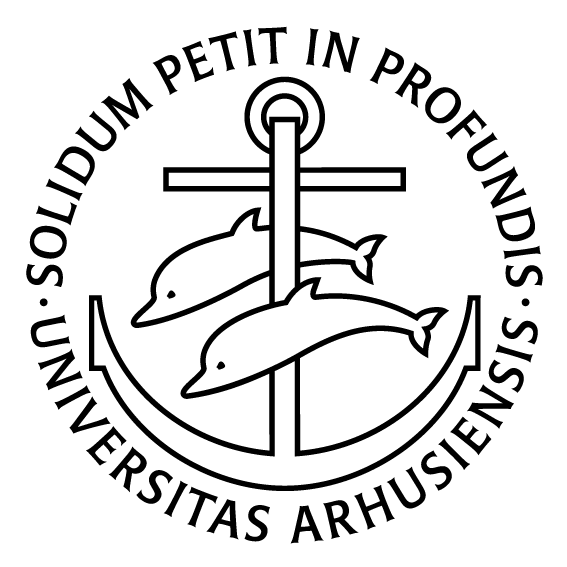
\includegraphics[width=0.5\textwidth]{ausegl_sort.png}
  \vspace{-10cm}
}

% \begin{centering}
  % 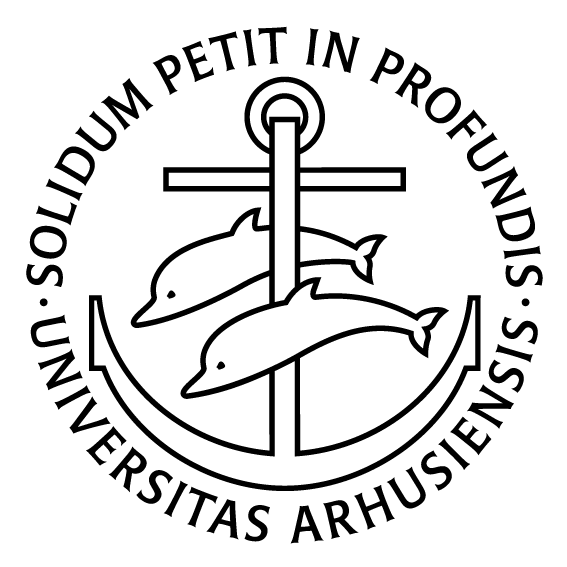
\includegraphics[width=0.5\textwidth]{ausegl_sort.png}
% \end{centering}
\vspace{0.5\textheight} % Whitespace between the title block and the publisher
\vfill
{\noindent Supervisor: Niels Lauritzen \hspace{2.5cm} 
\includegraphics{AU_logo.png}  }\\[\baselineskip] % Publisher and logo
}%}
% \endgroup
}

\begin{document}
% \maketitle
\pagenumbering{roman}
\titleGM
% \vfill
% Vejleder: Niels Lauritzen
% \strut\hfill
% 
\includegraphics[right]{AU_logo.png}
\newpage
\tableofcontents

\newpage
\pagenumbering{arabic}

\section*{Introduction}
Gröbner bases of ideals in multivariate polynomial rings are a vital tool when doing computational algebra and computational algebraic geometry. They often feature as an intermediary step in all sorts of problems, ranging from intersecting ideals and solving polynomial equations, to backwards kinematics and determining the behavior of chemical reaction networks\cite{IVA}. As such, the study of Gröbner bases have developed into a large field of its own.

In some situations, we may be interested in not just one ideal, but a family of ideals. For example, we might have a fixed algebraic curve, and we want to calculate the distance between a point and the curve. This can be done by computing a Gröbner basis for a system of equations, given by the Lagrange multipliers. Keeping the coordinates of the point as parameters, we would like to quickly compute this distance for many points. From a purely mathematical view, we might be interested in the behavior of a Gröbner basis as we change the base ring. Given an ideal $I$ in a polynomial ring $K[U][X]$, we would like to describe the Gröbner basis obtained from $I$, by evaluating each $u \in U$ to a fixed value. In this way, we can see $I$ as a parameterized family of ideals, with $\,U$ being the parameters. A parametric Gröbner basis is a Gröbner basis of $\,I$, which remains a Gröbner basis for some choices of values for $U$ and a comprehensive parametric Gröbner basis remains a Gröbner basis for all choices of values for $U$. See definition~\ref{def:par_grb} for the precise definition.

Volker Weispfenning introduced the notion of a comprehensive parametric\footnote{Our terminology differs from the original terminology. What Weispfenning called a \textit{comprehensive Gröbner basis} we call a \textit{comprehensive parametric Gröbner basis.}} Gröbner basis in~\cite{Weispfenning} in 1992 and gave an algorithm to compute them. He also gave some results on the computational complexity of this algorithm as well as some early applications. However, the computation of Gröbner bases, and by extension parametric Gröbner bases, is a difficult problem. Many optimizations and heuristics exist, which means the computation of Gröbner bases should be performed using highly optimized software. Reimplementing all this for parametric Gröbner bases might not be feasible. In 2006, Suzuki and Sato produced an algorithm for computing parametric Gröbner bases, that utilize existing software for computing Gröbner bases. Even though the theoretical complexity didn't change, the execution time certainly did, as the algorithm could exploit existing optimized algorithms for computing Gröbner bases. Kapur, Sun and Wang improved on this algorithm in 2010~\cite{KAPUR201327}\cite{10.1145/1837934.1837946}.

After parametric Gröbner bases were established, the search began for a unique object, a parametric analogue of the reduced Gröbner basis. Weispfenning introduced what he called a canonical comprehensive Gröbner basis in~\cite{WEISPFENNING2003669}, which only depends on the ideal and the monomial order on the variables and the parameters. However, no object comparable to the reduced Gröbner basis, which was independent of assumptions on the ground ring was found until Michael Wibmer introduced Gröbner covers in~\cite{grb_covers}. By drawing on machinery from modern algebraic geometry, including the language of sheaves and schemes, he found a parametric way of describing the reduced Gröbner basis of every specialization of the ideal in question, called Gröbner covers. He also proved the existence of a canonical Gröbner cover if $I$ is homogenous. This rather abstract paper was quickly followed up by~\cite{MONTES20101391}, which described an algorithm to compute Gröbner covers. It should be noted, that even though the canonical Gröbner cover described by Wibmer is unique in a mathematical sense, there is no canonical, finite description of it, without adding in some assumptions on the base ring.

The focus of this paper is to serve as an introduction to parametric Gröbner bases. First, we establish parametric Gröbner bases, Gröbner systems and some initial results on parametric Gröbner bases. In particular, a fundamental theorem by Kalkbrener\cite{Kalkbrener} on when a Gröbner basis remains a Gröbner basis after specialization, as well as a tool called pseudo-division. Then, we cover the algorithm introduced by Suzuki and Sato. From here, we move on to Gröbner covers as introduced by Wibmer, to give an introduction into this, quite different framing of parametric Gröbner bases. We tie this theory together with the Suzuki-Sato algorithm, and provide plenty of examples to help get a feeling for the subject. Finally, we cover some applications of parametric Gröbner bases and Gröbner covers.

We purposefully do not cover Kapur, Sun and Wangs algorithm nor the implementation of Wibmers theory by Antonio Montes\cite{MONTES20101391}. These are seen as refinements of the material already covered, and covering them would exceed the scope of this introduction. Instead, we focus on tying the algorithm of Suzuki and Sato to the theory of Wibmer. This is how modern implementations of parametric Gröbner bases are implemented\footnote{See \url{https://www.singular.uni-kl.de/Manual/latest/sing_1042.htm}}, but doesn't seem to be described in detail in the literature.

New contributions of this project include
\begin{itemize}
  \item Fixing edge-case bugs in the pseudocode in \cite{ss_algo}, see algorithm~\ref{alg:CGS_simple}
  \item Modifying the Suzuki-Sato algorithm to produce Gröbner covers, see theorem~\ref{thm:CGS}
  \item Placing pseudo-division as a central tool of Gröbner covers and comprehensive Gröbner bases, see section~\ref{sec:ps_div} and \ref{sec:ps_div_app}
  \item Identifying a mistake in~\cite{sturmfels} and fixing it using comprehensive Gröbner bases, see section~\ref{sec:bernd}
  \item A new implementation of comprehensive Gröbner bases in the Julia programming language with demonstrations of their applications\footnote{See \url{https://github.com/0708andreas/ParametricGroebnerBases.jl}}.
\end{itemize}

\newpage

\section{Preliminaries}
This project will assume familiarity with commutative ring theory and multivariate polynomials over fields. A familiarity with Gröbner bases will be beneficial, but we will introduce the necessary notations and definitions. Let $A$ be a Noetherian, commutative ring and $X = (x_{1}, x_{2}, \dots, x_{n})$ be an ordered collection of symbols. We denote the ring of polynomials in these variables $A[X]$. Given two (disjoint) sets of variables $X$ and $Y$, we will use $A[X, Y]$ to mean $A[X \cup Y]$, which is isomorphic to $A[X][Y]$. A monomial is a product of variables and a term is a monomial times a coefficient. We denote a monomial as $X^{v}$ for some $v \in \N^{n}$. For a polynomial \[f = \sum_{v \in \N^{n}} a_{v}X^{v}\] we denote the coefficient of the term $t = a_{v}X^{v}$ by $\coef(f, X^{v})$.

\begin{definition}[Monomial order, leading term]
  A \textit{monomial order} is a well-order\footnote{A total order, for which any chain $a > b > c > \dots$ must be finite.} $<$ on the set of monomials satisfying that $u < v \implies wu < wv$.

  Given a monomial order $<$ and a polynomial $f \in A[X]$, the \textit{leading term} of $f$ is the term with the largest monomial w.r.t. $<$ and is denoted by $\LT_{<}(f)$. If $\LT_{<}(f) = a\cdot m$ for some monomial $m$ and $a \in A$, then we denote $\LM_{<}(f) = m$ and $\LC_{<}(f) = a$. If $<$ is clear from context, it will be omitted.
\end{definition}

These definitions naturally extend to sets of polynomials, so given a set of polynomials $F \subset A[X]$, we denote $\LM_{<}(F) := \{\LM_{<}(f) \mid f \in F\}$. When $I \subset A[X]$ is an ideal, we use $\LM_{<}(I)$ to denote $\langle \LM_{<}(I) \rangle$ to ease notation, and similarly for $\LT_{<}(I)$. With this, we can give the definition of a Gröbner basis. Usually, this is done over a field, for a reference on Gröbner bases over rings, see \cite{loustaunau1994introduction}. The standard reference on Gröbner bases is \cite{IVA}.

\begin{definition}[Gröbner basis]
  Let $G \subset A[X]$ be a finite set of polynomials and $<$ be a monomial order. We say $G$ is a \textit{Gröbner basis} if
  $\langle \LT_{<}(G) \rangle = \LT_{<}(\langle G \rangle )$.
\end{definition}

Note, that if $A$ is a field, then it is enough that $\langle \LM_{<}(G) \rangle = \LM_{<}(\langle G \rangle)$. We say $G$ is a Gröbner basis for an ideal $I$ if $G$ is a Gröbner basis and $\langle G \rangle = I$. We will also have to use an alternative description of Gröbner bases.

\begin{definition}[Reduction modulo]
  Let $f, g \in A[X]$ be polynomials and $<$ be a term order. We say $f$ \textit{reduces modulo} $g$ if $\LT_{<}(g) \mid \LT_{<}(f)$, since in that case $\LT_{<}(\LC_{<}(g)\cdot f - p\cdot \LC_{<}(f) \cdot g) < \LT_{<}(f)$ where $\LM_{<}(f) = p \cdot \LM_{<}(g)$. We say a polynomial reduces modulo a set of polynomials if it reduces modulo any polynomial in the set. We say a polynomial \textit{reduces to zero} if there is a chain of reductions that end in the zero polynomial.
\end{definition}

\begin{theorem}\label{thm:grb}
  Let $G \subset A[X]$. Then $G$ is a Gröbner basis if and only if every polynomial in $\langle G \rangle$ reduces to 0 modulo $G$.
\end{theorem}
\begin{proof}
  A good exercise.
\end{proof}

A Gröbner basis need not be unique. Indeed, given a Gröbner basis G, we can add any element of $\langle G \rangle$ to $G$ and it is still a Gröbner basis. However, reduced Gröbner bases are unique.

\begin{definition}[Reduced Gröbner basis]
  A Gröbner basis $G$ is called \textit{reduced} if, for all $g \in G$, $g$ is a monic polynomial (i.e. $\LC_{<}(g) = 1$) and the only term of $g$ in $\LT_{<}(\langle G \rangle)$ is $\LT_{<}(g)$.
\end{definition}
\begin{theorem}
  Let $I \subset k[X]$ be an ideal in a polynomial ring over a field. Then there is a unique reduced Gröbner basis of $I$.
\end{theorem}

It is worth noting, that the second condition of reduced Gröbner bases is equivalent to saying that every term of $g$ is irreducible modulo $G$, except for its leading term.

\newpage

\section{Definitions and initial results}

\subsection{Parametric Gröbner bases and their motivation}
Gröbner bases are a central tool when doing almost any computations on ideals in multivariate polynomial rings. Gröbner bases helps us to decide ideal membership, and when using a suitable term order it helps us to intersect ideals, eliminate variables, decide radical membership etc. Sometimes, we wish to study a family of ideals, parameterized by some variables. We could for instance ask for which values of $a$ and $b$ we have $ax - 1 \in \langle bx - 1 \rangle$. While this example is admittedly simple, answering such questions in general would require us to be able to describe a Gröbner basis for a parameterized ideal, no matter what value the parameters take. In this simple example, $ax - 1 \in \langle bx - 1 \rangle$ if and only if $a = b$ unless $b = 0$ in which case the inclusion hold for any value of $a$. This corresponds to the observation that $bx - 1$ is a Gröbner basis for the ideal and when $b=0$, 1 is a Gröbner basis.

We will gradually look at more structured ways of describing the Gröbner basis of a parameterized ideal. The first definition was introduced by Volker Weispfenning in~\cite{Weispfenning}.

\begin{definition}[Comprehensive parametric Gröbner basis]\label{def:par_grb}
  Let $A$ be a commutative, Noetherian ring, $k_{1}$ be a field, $X$ be a set of variables and let $F \subset A[X]$ be a finite set of polynomials. A \textit{comprehensive parametric Gröbner basis} of $\langle F \rangle$ is a finite set of polynomials $G \subset \langle F \rangle$ such that $\sigma(G)$ is a Gröbner basis of $\langle \sigma(\langle F \rangle) \rangle$ for any ring homomorphism $\sigma : A \to k_{1}$. Here $\sigma(f)$ for an $f \in A[X]$ denotes the coefficient-wise application of $\sigma$ on $f$.
\end{definition}
\textit{Remark. }Most of this text will focus on the special case when $k$ is a field contained in $k_{1}$, $U$ is another set of variables with $U \cap X = \emptyset$ and $A = k[U]$. Then $\sigma : k[U] \to k_{1}$ corresponds to a choice of value for each variable in $U$. Since $k[U][X]$ is isomorphic to $k[X, U]$, we will often refer to parametric Gröbner bases of an ideal $I \subset k[X, U]$. It is also important to see, that $\langle \sigma(F) \rangle = \langle \sigma(\langle F \rangle) \rangle$ for any finite $F \subset A[X]$ and any specialization $\sigma$.

For example, consider the ideal $I = \langle ux + y, y^{2} + 1 \rangle \subset \C[u][x, y]$. The given generators form a Gröbner basis of $I$ w.r.t.\ the lexicographic monomial order, and also for every choice of $u$, except $u = 0$. In this case, the generators become $\{y, y^{2} + 1\}$, which is not a Gröbner basis. Indeed, $\langle y, y^{2} + 1 \rangle = \C[x, y]$, so $1 \in \langle \LM(\langle y, y^{2} + 1 \rangle) \rangle$. But $\langle \LM(\{y, y^{2} + 1\}) \rangle = \langle y \rangle$, which does not contain 1.

We call a ring homomorphism $\sigma : k[U] \to k_{1}$ a \textit{specialization}. Since $\sigma|k : k \to k_{1}$ is always injective, we can assume without loss of generality that $k \subset k_{1}$ and that $\sigma$ restricted to $k$ is the identity, i.e. $\sigma|k = id$. By the linearity of $\sigma$, we can characterize $\sigma$ uniquely by its image of $\,U$. Thus, we can identify $\{\sigma : k[U] \to k_{1} \mid \sigma \text{ is a ring hom.}\}$ with the affine space $k_{1}^{|U|}$. For $\alpha \in k_{1}^{|U|}$ we'll denote the corresponding map
\[\sigma_{\alpha}(u_{i}) = \alpha_{i} \quad \text{for $u_{i} \in U$}\] extended linearly.

It should be noted, that for computing Gröbner bases of ideals in the ring $k[U][X]$, it suffices to compute a Gröbner basis of the ideal, just viewing it as an ideal in $k[X, U]$ with respect to a monomial order where $X^{v_{1}} > U^{v_{2}}$ for all vectors of natural numbers $v_{1}, v_{2}$. This is proven in lemma~\ref{lem:block_order}.

\begin{example}\upshape
  The behavior of the ideal of leading monomials is highly erratic under specializations. If $F$ is a generating set for some ideal $I \subset A[X]$ and $\sigma : A \to k_{1}$ is a specialization, then we can have all the following scenarios:
  \begin{itemize}
    \item $\langle \LM(\sigma(I)) \rangle = \langle \LM(I) \rangle$ \\ If $F = \{x^{2} + u\} \subset \C[u][x]$ and $\sigma : \C[u] \to \C$ sets $\sigma(u) = 0$, then $\sigma(F) = \{x^{2}\}$, hence $\langle x^{2} \rangle = \langle \LM(\sigma(I)) \rangle = \langle \LM(I) \rangle = \langle x^{2} \rangle$.

    \item $\langle \LM(\sigma(I)) \rangle \subsetneq \langle \LM(I) \rangle$ \\ If $F = \{ux, y\} \subset \C[u][x]$ and $\sigma : \C[u] \to \C$ sets $\sigma(u) = 0$, then $\sigma(F) = \{y\}$, hence $\langle y \rangle = \langle \LM(\sigma(I)) \rangle \subsetneq \langle \LM(I) \rangle = \langle x, y \rangle$.

    \item $\langle \LM(I) \rangle \subsetneq \langle \LM(\sigma(I)) \rangle$ \\ If $F = \{ux^{2} + x\} \subset \C[u][x]$ and $\sigma : \C[u] \to \C$ sets $\sigma(u) = 0$, then $\sigma(F) = \{x\}$, hence $\langle x^{2} \rangle = \langle \LM(I) \rangle \subsetneq \langle \LM(\sigma(I)) \rangle = \langle x \rangle$.

    \item $\langle \LM(I) \rangle \nsubset \langle \LM(\sigma(I)) \rangle$ and $\langle \LM(\sigma(I)) \rangle \nsubset \langle \LM(I) \rangle$ \\ If $F = \{ux^{2} + x, uy\} \subset \C[u][x]$ and $\sigma : \C[u] \to \C$ sets $\sigma(u) = 0$, then $\sigma(F) = \{x\}$, hence $\langle \LM(I) \rangle = \langle x^{2}, y \rangle$ which is neither a subset nor a superset of $\langle \LM(\sigma(I)) \rangle = \langle x \rangle$.
  \end{itemize}
\end{example}

% \begin{example}\upshape
%   Consider the ideal $I = \langle ux - 1, vx - 1 \rangle \subset \C[u, v][x, y]$ and a specialization $\sigma : \C[u, v] \to \C$. To analyze the behaviour of $I$ under different specializations, let's split into cases.

%   \begin{enumerate}
%     \item If either $\sigma(u) = 0$ or $\sigma(v) = 0$, then $\langle \sigma(I) \rangle = \langle 1 \rangle \subset \C[x, y]$. If $\sigma(u) = 0$, then $\sigma(ux - 1) = -1$, hence the generators above form a Gröbner basis of $\langle I \rangle$. The other polynomial becomes redundant, so we don't have a reduced Gröbner basis.

%     \item If $\sigma(u) = \sigma(v)$, then $\langle \sigma(I) \rangle = \langle \sigma(u)x - 1 \rangle$. In this case the generators also form a Gröbner basis.

%     \item If $\sigma(u) \neq \sigma(v)$ and neither of them are 0, then $\sigma(v)(\sigma(u)x - 1) - \sigma(u)(\sigma(v)x - 1) = \sigma(v) - \sigma(u) \in \langle \sigma(I) \rangle$, hence $\langle \sigma(I) \rangle = \langle 1 \rangle$. In this case the generators do not form a Gröbner basis of $\langle \sigma(I) \rangle$.
%   \end{enumerate}

%   The reduced Gröbner basis of $I$ is $\{u - v, ux - 1\}$, which always specializes to a Gröbner basis, as can be seen above. However, it is not always enough to compute a reduced Gröbner basis.

%   Consider the ideal $J = \langle ux^{2} + y, y^{2} + 1 \rangle$, where the generators form the reduced Gröbner basis of $J$. And indeed, whenever $\sigma(u) \neq 0$, it specializes to the reduced Gröbner basis of $\langle \sigma(J) \rangle$. However, when $\sigma(u) = 0$, we get $\langle \sigma(J) \rangle = \langle 1 \rangle$, but $\sigma(\{ux^{2} + y, y^{2} + 1\}) = \{y, y^{2} + 1\}$, which is not a Gröbner basis.

%   $G = \{ax^{2} + y + 1, bx^{2} + y + 1, y-1\}$
% \end{example}

As can be seen from the example of $\{ux + y, y^2 + 1\}$, a set of generators can form a parametric Gröbner basis for a restricted set of specializations. Sometimes we are only interested in a subset of specializations. Since a specialization is uniquely determined by its image of the parameters, we use subsets of $k_{1}^{|U|}$ to describe these restrictions. Since the end goal of this is to compute parametric Gröbner bases, we want to work with subsets that can be described in a computationally feasible way. We use the Zariski topology, where closed sets (and hence open sets) can be described by a finite set of polynomials.

\begin{definition}[Vanishing sets \& locally closed sets]
  Let $k \supset k_{1}$ be fields and $E \subset k[X]$. Then the \textit{vanishing set} of $E$ is $\V(E) := \{v \in k_{1}^{n} \mid e(v) = 0 \;\; \forall e \in E\}$.  If $f \in k[X]$ we write $\V(f)$ to mean $\V(\{f\})$.

  A \textit{locally closed set}\footnote{Called such because if $\,Y = C \setminus D$ is a locally closed set, then $Y$ is a closed set in the subspace topology on $D^{\complement}$} is a set of the form $\V(E) \setminus \V(N)$ for two closed sets $\V(E)$ and $\V(N)$.
\end{definition}

For example, when working over $k = \R$, we have $\V(0) = \R^{n}$, $\V(1) = \emptyset$, and $\V(x^{2} + y^{2} - 1)$ is the unit circle in $\R^{2}$. $\V(x^{2} + y^{2} - 1) \setminus \V(x)$ is the unit circle in $\R^{2}$ with the  $x$-axis removed. In the Zariski topology a subset $C \subset k_{1}^{n}$ is closed if and only if $C = \V(E)$ for some $E \subset k[X]$. It should be noted, that $\V(E) = \V(\langle E \rangle)$ for all $E \subset k[X]$.

\begin{definition}[Parametric Gröbner basis]
  Let $k \supset k_{1}$ be fields, let $X$ be a set of variables, let $F \subset k[U][X]$ be a finite set of polynomials and let $Y \subset k_{1}^{|U|}$ be a locally closed set. A \textit{parametric Gröbner basis} of $\langle F \rangle$ on $Y$ is a finite set of polynomials $G \subset \langle F \rangle$ such that $\sigma(G)$ is a Gröbner basis of $\langle \sigma(\langle F \rangle) \rangle$ for any ring homomorphism $\sigma_{\alpha} : k[U] \to k_{1}$ with $\alpha \in Y$.
\end{definition}
\begin{definition}[Gröbner system]
  Let $Y$ be a locally closed set and $F, G \subset k[U][X]$ be finite sets. Then $(Y, G)$ is called a \textit{segment of a Gröbner system for $F$} if $\sigma_{\alpha}(G)$ is a Gröbner basis of $\langle \sigma_{\alpha}(F) \rangle$ for all $\alpha \in Y$. A set $\{(Y_{1}, G_{1}), \dots, (Y_{t}, G_{t})\}$ is called a \textit{Gröbner system} if each $(Y_{i}, G_{i})$ is a segment of a Gröbner system.

  We call the locally closed sets $Y_{i}$ for the $\textit{conditions}$ on a segment.

  A Gröbner system $\{(Y_{1}, G_{1}), \dots, (Y_{t}, G_{t}))\}$ is called \textit{comprehensive}, if $\bigcup_{i=1}^{\,t}Y_{i} = k_{1}^{|U|}$. We also say a Gröbner system is \textit{comprehensive on $L \subset k_{1}^{|U|}$} if $\bigcup_{i=1}^{t}Y_{i} = L$.
\end{definition}

We will sometimes call a triple $(E, N, G)$ for a segment of a Gröbner system. By this we mean that $(V(E) \setminus V(N), G)$ is a segment of a Gröbner system. Do also note, that for segments of a Gröbner system, we relax the restriction that $G \subset \langle F \rangle$ to just $G \subset A[X]$.

Gröbner systems and parametric Gröbner bases are restricted to ideals in $k[U][X]$ instead of over a more general ring $A[X]$. Section~\ref{sec:grb_covers} will cover the more general case.

\begin{example}\upshape
  Consider again the ideal $J = \langle ux^{2} + y, y^{2} + 1 \rangle \subset \C[u][x, y]$. It shouldn't be hard to convince yourself that the given generators form a Gröbner basis under any specialization where $\sigma(u) \neq 0$. For the specialization setting $\sigma(u) = 0$, we have $\langle \sigma(J) \rangle = \langle 1 \rangle$. Hence, we have the following comprehensive Gröbner system:
  \[\{(\V(0) \setminus \V(u), \{ux^{2} + y, y^{2} + 1\}), \quad (\V(u) \setminus \V(1), \{1\})\}\]

  The first segment gives a parametric Gröbner basis of $J$ on $\V(0) \setminus \V(u)$. But since $1 \notin \J$, the second segment does not give a parametric Gröbner basis of $J$ on $\V(u) \setminus \V(1)$. However, $-y(ux^{2} + y) + (y^{2} + 1) = -ux^{2}y + 1 \in J$ specializes to $1$ when $\sigma(u) = 0$. Hence, we also have the following Gröbner system, which also gives a comprehensive parametric Gröbner basis:
  \[\{(\V(0) \setminus \V(1), \{ux^{2} + y, y^{2} + 1, -ux^{2}y + 1\})\}\]
\end{example}

\begin{definition}[Leading coefficient w.r.t.\ variables]
  Let $f \in k[X, U]$. Then $\LT_{U}(f)$ denotes the leading term of $f$, when we see $f$ as an element of $k[U][X]$. Similarly, the leading coefficient of $f \in k[U][X]$ is $\LC_{U}(f)$ and the leading monomial is $\LM_{U}(f)$.
\end{definition}

Note that $\LC_{U}(f) \in k[U]$, i.e.\ the leading term is a polynomial in $k[U]$ times a monomial in $X$. For example, the polynomial $f = ux + vx + 1 \in C[x, u, v]$ has $\LC_{\{u, v\}}(f) = u + v$, $\LM_{\{u, v\}}(f) = x$ and $\LT_{\{u, v\}}(f) = (u+v)x$.

From this point, we assume that the monomial order on $k[X, U]$ satisfies $X^{v_{1}} > U^{v_{2}}$ for all $v_{1} \in \N^{|X|}$ and $v_{2} \in \N^{|U|}$. We will write this property as $X \gg U$. This monomial order restricts to a monomial order on $k[X]$, denoted by $<_{X}$. Note that this assumption is not too restrictive, as we're usually only interested in a certain monomial order on the variables, since the parameters will be specialized away anyway. Thus, for a given monomial order $<_{X}$, we can construct a suitable monomial order on $k[X, U]$, by using $<_{X}$ and breaking ties with any monomial order on $k[U]$. The lexicographic order with $X > U$ satisfies $X \gg U$. The reason for this assumption is the following lemma:

\begin{lemma}\label{lem:block_order}
  Let $<$ be a monomial order on $k[X, U]$ such that $X \gg U$, let $I \subset k[X, U]$ be an ideal and let $G = \{g_{1}, \dots, g_{n}\}$ be a Gröbner basis of $I$ w.r.t.\ $<$. Then $G$ can be seen as a Gröbner basis of $\,I \subset k[U][X]$ w.r.t.\ the restricted monomial order $<_{X}$.
\end{lemma}
\begin{proof}
  Let $f \in I \subset k[X, U]$., then we need to prove that $\LT_{U}(f) \in \langle \LT_{U}(G) \rangle$. As $G$ is a Gröbner basis of $I$ in $k[X, U]$, we can write
  \[ f = \sum_{i=1}^{n} h_{i} g_{i} \]
  where $\LM(f) \geq \LM(g_{i}, h_{i})$ for each $i$. Since $X \gg U$ this implies $\LM_{U}(f) \geq \LM_{U}(g_{i}, h_{i})$ for each i. Because of the inequality $\LM_{U}(f) \geq \LM_{U}(g_{i} h_{i})$, the leading term of $f$ can only be produced by leading terms of $g_{i}h_{i}$. Now, the equation above still holds when we see $f, g_{1}, \dots, g_{n}, h_{1}, \dots, h_{n}$ as elements of $k[U][X]$. Let $J = \{i \in \{1, \dots, n\} \mid \LM_{U}(h_{i} g_{i}) = \LM_{U}(f)\}$. Since $\LT_{U}(g_{i} h_{i}) = \LT_{U}(g_{i})\LT_{U}(h_{i})$, we have
  \[\LT_{U}(f) = \sum_{i \in J} \LT_{U}(h_{i}) \LT_{U}(g_{i})\]
  so $\LT_{U}(f) \in \langle \LT_{U}(G) \rangle$, and so $G$ is a Gröbner basis of $I \subset k[U][X]$.
\end{proof}











\subsection{Pseudo-division}\label{sec:ps_div}
The division algorithm for polynomial rings over fields form the basis of most of the applications of Gröbner bases. One could even say that having a well-behaved remainder under the division algorithm is one of the primary motivations behind Gröbner bases. Pseudo-division will turn out to be equally important in the parametric setting. The idea is straight-forward. Suppose you want to divide $ax$ by $bx$ in $k[a, b][x]$. Since $b$ does not divide $a$, it seems we are stuck. But that is only due to the nature of the ring we work over (specifically that it's not a field) rather than the structure of the polynomials. Had $a$ and $b$ been any non-zero field elements, the division would be easy.

Pseudo-division is a way to overcome the fact, that our ground ring may not be a field. The idea is to allow ourselves to scale the polynomial by an appropriate scalar from the ground ring. In the case above, we can't divide $ax$ by $bx$, but we can divide $bax$ by $bx$ and get a remainder of zero. Pseudo-division in a restricted setting over $k[U][X]$ can be found in~\cite{IVA}. I am not aware that the rest of the results in this subsection appear in literature, but they have been extracted from proofs of other theorems in~\cite{grb_covers},~\cite{MONTES20101391}.

\begin{definition}[Pseudo-division]
  Let $f, f_{1}, f_{2}, \dots, f_{n}, g_{1}, g_{2}, \dots, g_{n}, r \in A[X]$ be polynomials and let $c \in A$. A \textit{pseudo-division of $f$ modulo $g_{1}, \dots, g_{n}$} is a relation
  \[cf = r + \sum_{i=1}^{n} f_{i}g_{i}\]
  where the following is satisfied:
  \begin{enumerate}
    \item $c = \prod_{j\in J} \LC(g_{j})^{p_{j}}$ for some subset $J \subset \{1, 2, \dots, n\}$ and powers $p_{j} \in \N$.
    \item $\LM(f_{i})\LM(g_{i}) \leq \LM(f)$ for all $i \in \{1, 2, \dots, n\}$.
    \item No term of $r$ is divisible by $\LM(g_{i})$ for any $i$.
    \item $\coef(f_{i}, m) \in \langle \coef(f, m') \mid m' \geq \LM(g_{i}m) \rangle$ for all $i \in \{1, 2, \dots, n\}$ and monomials $m$.
  \end{enumerate}
  We call $r$ a \textit{pseudo-remainder} and the $f_{i}$'s are called \textit{pseudo-quotients}.
\end{definition}


\begin{theorem}\label{thm:exi_pseudo}
  Let $f, g_{1}, g_{2}, \dots, g_{n} \in A[X]$ be polynomials. Then there exists a pseudo-division of $f$ modulo $g_{1}, \dots, g_{n}$.
\end{theorem}
\begin{proof}
  See the appendix, section \ref{app:pseudo}
\end{proof}

Pseudo-division allows us to overcome the problem, that our ground ring isn't a field, but we still have to be careful. If $b$ happened to be zero, then we cannot divide $ax$ by $bx$. Hence, we need some assumptions on the leading terms we divide with. The reason is that, after specialization, a pseudo-division turns into a regular multivariate division. Hence, parametric Gröbner bases and pseudo-division inherit all the nice properties Gröbner bases has under regular division.

\begin{lemma}\label{lem:ps_div_to_div}
  Let $f \in A[X]$, let $\{g_{1}, \dots, g_{n}\} \subset A[X]$, let $\sigma : A \to k_{1}$ be a ring homomorphism and let
  \[cf = r + \sum_{i=1}^{n}f_{i}g_{i}\]
  be a pseudo-division. Then
  \[\sigma(cf) = \sigma(r) + \sum_{i=1}^{n} \sigma(f_{i})\sigma(g_{i})\]
  satisfies $\LM(\sigma(f_{i} g_{i})) \leq \LM(\sigma(f))$. Furthermore, if $\sigma(\LC(g_{i})) \neq 0$ for all $i$, then either $\sigma(r) = 0$ or none of the terms of $\sigma(r)$ is divisible by any leading term of the $\sigma(g_{i})$'s.
\end{lemma}
\begin{proof}
  The first equality follows directly since $\sigma$ is a ring homomorphism. For the inequality $\LM(\sigma(f_{i} g_{i})) \leq \LM(\sigma(f))$, we have the fourth condition from pseudo-divisions: $\coef(f_{i}, m) \in \langle \coef(f, m') \mid m' \geq m \LM(g_{i}) \rangle$. Hence for any monomial $m$ with $m\LM(g_{i}) \geq \LM(\sigma(f))$, we have $\sigma(\coef(f_{i}, m \LM(g_{i}))) = 0$, since $\langle \coef(f, m) \mid m \geq \LM(\sigma(f)) \rangle = \langle 0 \rangle$.

  For the remainder, we have from pseudo-division that no term of $r$ is divisible by any $\LT(g_{i})$. Assuming $\sigma(\LC(g_{i})) \neq 0$ for all $i$, we have $\LM(g_{i}) = \LM(\sigma(g_{i}))$ for all $i$. Hence, no term of $\sigma(r)$ is divisible by any $\LM(\sigma(g_{i}))$, and since we work over a field, no term of $\sigma(r)$ is divisible by any $\LT(\sigma(g_{i}))$.
\end{proof}


Since remainders modulo a Gröbner basis $G$ are unique, we have that $f \in \langle G \rangle$ if and only if $f$ leaves a remainder of $0$ under division modulo $G$. We have the following analogous statement for parametric Gröbner bases and pseudo-division.

\begin{lemma}\label{lem:ps_rem_unique}
  Let $(Y, G)$ be a segment of a parametric Gröbner basis with $G = \{g_{1}, \dots, g_{n}\} \subset A[X]$, and assume that $\sigma_{\alpha}(\LC(g)) \neq 0$ for all $\alpha \in Y$ and $g \in G$. Let $f \in A[X]$ and let
  \[cf = r + \sum_{i=1}^{n} f_{i} g_{i}, \quad c'f = r' + \sum_{i=1}^{n} f'_{i} g_{i}\]
  be pseudo-divisions. Then
  \[\sigma_{\alpha}(r'c) = \sigma_{\alpha}(rc')\]
  for all specializations $\sigma_{\alpha}$ with $\alpha \in Y$. Furthermore, $\sigma_{\alpha}(f) \in \langle \sigma_{\alpha}(G) \rangle$ if and only if $\sigma_{\alpha}(r) = 0$.
\end{lemma}
\begin{proof}
  Consider
  \begin{align*}
    0 &= \sigma_{\alpha}(c' c f) - \sigma_{\alpha}(c' c f) \\
      &= \sigma_{\alpha}(cr') - \sigma_{\alpha}(c'r) + \sum_{i=1}^{n}\left(\sigma_{\alpha}(c f_{i}') - \sigma_{\alpha}(c' f_{i})\right)\sigma_{\alpha}(g_{i}).
  \end{align*}
  Since $\sum_{i=1}^{n}(\sigma_{\alpha}(c f_{i}') - \sigma_{\alpha}(c' f_{i}))\sigma_{\alpha}(g_{i}) \in \langle \sigma_{\alpha}(G) \rangle$, we must have $\sigma_{\alpha}(c' r) - \sigma_{\alpha}(c r') \in \langle \sigma_{\alpha}(G) \rangle$. If $\sigma_{\alpha}(c't) - \sigma_{\alpha}(cr') \neq 0$ then, since $\sigma_{\alpha}(G)$ is a Gröbner basis, that would imply that the leading term of $\sigma_{\alpha}(c' r) - \sigma_{\alpha}(c r')$ is divisible by some $\LM(\sigma_{\alpha}(g_{i}))$. But that would imply some term of either $\sigma_{\alpha}(c' r)$ or $\sigma_{\alpha}(c r')$ is divisible by that $\LM(\sigma_{\alpha}(g_{i}))$. Since $\LM(\sigma_{\alpha}(g_{i})) = \LM(g_{i})$ and no term of $r$ is divisible by any $\LM(g_{i})$ (by the properties of pseudo-division), this cannot happen. Hence, $\sigma_{\alpha}(c' r) - \sigma_{\alpha}(c r') = 0$.

  For the last assertion, if $\sigma_{\alpha}(r) = 0$, then clearly $\sigma_{\alpha}(f) \in \langle \sigma_{\alpha}(G) \rangle$ since $\sigma_{\alpha}(c)$ is invertible. On the other hand, if $\sigma_{\alpha}(f) \in \langle \sigma_{\alpha}(G) \rangle$, find a pseudo-reduction
  \[c f = r + \sum_{i=1}^{n} g_{i} f_{i}\]
  Then, since $\sigma_{\alpha}(c) \neq 0$ for any $\alpha \in Y$, by lemma~\ref{lem:ps_div_to_div} we get that
  \[\sigma_{\alpha}(c)\sigma_{\alpha}(f) = \sigma_{\alpha}(r) + \sum_{i=1}^{n} g_{i} f_{i}\]
  where no term of $\sigma_{\alpha}(r)$ is divisible by any leading term of $\sigma_{\alpha}(G)$. Since $\sigma_{\alpha}(G)$ is a Gröbner basis, and $\sigma_{\alpha}(c) \sigma_{\alpha}(f) \in \langle \sigma_{\alpha}(G) \rangle$, this implies $\sigma_{\alpha}(r) = 0$.
\end{proof}

\begin{example}\upshape
  Consider the comprehensive parametric Gröbner basis $G = \{ ax + y, bx + y, (a - b)y \} \subset \C[a, b, c][x, y]$ and the element $f = cxy + 1 \in \C[a, b, c][x, y]$. On the segment $\V(0) \setminus \V(ab(a-b))$, we can find a pseudo-reduction. First, reduce the term $cxy$ using $ax + y$:
  \[ (a)(cxy + 1) = (cy)(ax + y) - cy^{2} + a \]
  leaving a remainder of $\,-cy^{2} + a$. This remainder can be reduced using $(a - b)y$:
  \[(a-b)(a)(cxy + 1) = (a-b)(cy)(ax + y) - (cy)((a - b)y) + a^{2} - ab \]
  giving us the multiplier $c = a(a - b)$ and remainder $r = a^{2} - ab$.

  We could also have reduced the term $cxy$ using $(a - b)y$:
  \[(a-b)(cxy + 1) = (cx)((a-b)y) + a - b \]
  giving us a multiplier $c' = (a - b)$ and remainder $a - b$. We see that $c r' = (a-b)(a^{2} - ab) = (a - b)((a-b)a) = c' r$ in accordance with the theorem above.

  If the segment induces relations between leading coefficients, this might show up in the pseudo-remainders. Consider the segment $(\V(a - b), \{ax + 1, bx + 1\})$ and the polynomial $abx$. Here, we find two different pseudo-remainders:
  \begin{align*}
    abx = (b)(ax + 1) - b \\
    abx = (a)(bx + 1) - a
  \end{align*}
  In accordance with the theorem, we have that $\sigma_{\alpha}(a) = \sigma_{\alpha}(b)$ for all $\alpha \in \V(a - b)$. Do note, that for $\alpha \notin \V(a - b)$, $\sigma_{\alpha}(\{ax + 1, bx + 1\})$ is not a Gröbner basis, hence the theorem does not apply here.
\end{example}

Finally, to fully establish the correspondence between pseudo-division before specialization and division after specialization, we have the following: if we have a Gröbner basis $\sigma(G)$ after specialization, then any division modulo $G$ ``lifts'' to a pseudo-division before specialization. That is the content of this rather technical lemma.

\begin{lemma}\label{lem:div_to_ps_div}
  Let $G = \{g_{1}, \dots, g_{n}\} \subset A[X]$, let $f \in \langle G \rangle$ and let $\sigma : A \to K_{1}$ be a specialization such that $\sigma(\LC(g_{i})) \neq 0$ for all $i$. If $\,\sigma(f)$ reduces to zero mod $\sigma(g_{1}), \dots, \sigma(g_{n})$, then there is some $h \in \langle G \rangle$ and $\,b \in A \setminus \ker(\sigma)$ such that $\sigma(bf) = \sigma(h)$ and $\,\LM(h) = \LM(\sigma(f))$.
\end{lemma}
\begin{proof}
  The proof is by induction on the monomial order $<$ in $\LM(\sigma(f))$. The base case is $\sigma(f) = 0$, in which case we can choose $h = 0 \in \langle G \rangle$ and $b = 1$.

  Now, let $\sigma(f) \neq 0$ reduce to zero mod $\sigma(g_{1}), \dots, \sigma(g_{n})$, and suppose for every $f' \in \langle G \rangle$ with $\LM(\sigma(f')) < \LM(\sigma(f))$, there is some $h' \in \langle G \rangle$ and $b \in A \setminus \ker(\sigma)$ such that $\sigma(b'f') = \sigma(h')$ and $\LM(h') = \LM(\sigma(f'))$. Let
  \[\sigma(f) = \frac{\LC(\sigma(f))}{\LC(\sigma(g_{i}))} \sigma(g_{i}) + r\]
  with $\LM(r) < \LM(\sigma(g))$ be the first step of the reduction to zero. Since $\sigma(\LC(g_{i})) \neq 0$, we have that $\LC(\sigma(g_{i})) = \sigma(\LC(g_{i}))$. Then we have
  \begin{align*}
    \sigma(f) &= \frac{\LC(\sigma(f))}{\sigma(\LC(g_{i}))} \sigma(g_{i}) + r \iff \sigma(\LC(g_{i}) f) = \LC(\sigma(f)) \sigma(g_{i}) + \LC(g_{i})r
  \end{align*}
  Thus, $\LC(\sigma(f)) = \sigma(\coef(f, \LM(\sigma(f))))$, and so
  \[f' = \LC(g_{i})f - \coef(f, \LM(\sigma(f))) g_{i} \in \langle G \rangle\]
  satisfies either $\sigma(f') = 0$ or $\LM(\sigma(f')) < \LM(\sigma(f))$. In the first case, we've reached the base case, so we are done. Otherwise, $\sigma(f')$ is reducible to zero mod $\sigma(g_{1}), \dots, \sigma(g_{n})$ via the rest of the reduction of $\sigma(f)$, so we can find $b' \in A \setminus \ker(\sigma)$ and $h' \in \langle G \rangle$ such that $\LM(h') = \LM(\sigma(f'))$ and $\sigma(b' f') = \sigma(h)$. Then let $b = b' \LC(g_{i})$ and $h = h' + b' \coef(f, \LM(\sigma(f))) g_{i}$, so
  \begin{align*}
    \sigma(b f) &= \sigma(\LC(g_{i}) b' f) \\
           &= \sigma(b' (f' + \coef(f, \LM(\sigma(f))) g_{i})) \\
           &= \sigma(h' + b' \coef(f, \LM(\sigma(f))) g_{i}) \\
           &= \sigma(h)
  \end{align*}
  and $\LM(h) = \LM(g_{i}) = \LM(\sigma(g_{i})) = \LM(\sigma(f))$. Finally, since $b', \LC(g_{i}) \notin \ker(\sigma)$, we have $b \notin \ker(\sigma)$. This uses that $\ker(\sigma)$ is a prime ideal, which is true since its codomain is a field.
\end{proof}














\subsection{A criterion on stability}
In this section we will prove a criterion to decide when a Gröbner basis $G$ of an ideal $\langle F \rangle$ maps to a Gröbner basis $\sigma(G)$ of the ideal $\langle \sigma(F) \rangle$. This is theorem 3.1 in \cite{Kalkbrener}.

\begin{lemma}\label{lem:grb_iff_reduc_to_z}
  Let $G$ be a Gröbner basis of an ideal $\langle F \rangle \subset A[X]$ w.r.t. $<$, let $\sigma : A \to K$ be a ring homomorphism to a field $K$ and set $\,G_{\sigma} = \{g \in G \mid \sigma(\LC(g)) \neq 0\} = \{g_{1}, g_{2}, \dots, g_{l}\} \subset A[X]$. Then $\sigma(G_{\sigma})$ is a Gröbner basis of the ideal $\langle \sigma(F) \rangle$ w.r.t. $<_{X}$ if and only if $\sigma(g)$ is reducible to 0 modulo $\sigma(G_{\sigma})$ for every $g \in G$.
\end{lemma}
\begin{proof}
  First, we prove ``$\Longrightarrow$'': Suppose $\sigma(G_{\sigma})$ is a Gröbner basis of $\langle \sigma(F) \rangle$. Since $\sigma(g) \in \langle \sigma(F) \rangle$, we get that $\sigma(g)$ reduces to zero modulo any Gröbner basis of $\langle \sigma(F) \rangle$ by theorem~\ref{thm:grb}, in particular $\sigma(G_{\sigma})$.

  Next, we prove ``$\Longleftarrow$'': Assume that $\sigma(g)$ is reducible to 0 modulo $G_{\sigma}$ for every $g \in G$ and let $f \in \langle F \rangle$ such that $\sigma(f) \neq 0$. It's enough to show that
  \[\exists\, h \in \langle F \rangle : \sigma(\LC(h)) \neq 0 \land \LM(h) \mid \LM(\sigma(f)).\]
  Indeed, since $G$ is a Gröbner basis of $\langle F \rangle$, that implies there is some $g \in G$ such that $\LM(g) \mid \LM(h)$ and $\LM(h) = \LM(\sigma(h)) \mid \LM(\sigma(f))$. Furthermore, since $\LC(g) \mid \LC(h)$ and $\sigma(\LC(h)) \neq 0$, we have that $\sigma(\LC(g)) \neq 0$, hence $\LT(\sigma(g)) \mid \LT(\sigma(f))$. Thus, if the above holds for any $f$, then $\sigma(G)$ is a Gröbner basis of $\langle \sigma(F) \rangle$. We prove this claim by induction on $<_{X}$.

  The base case is when $\LM(f) = 1$, which means $f \in A$. Since we assumed $\sigma(f) \neq 0$, we have $\LM(\sigma(f)) = \LM(f)$ and $\sigma(\LC(f)) \neq 0$.

  Now, the induction step. Let $f \in \langle F \rangle$ with $\sigma(\LC(f)) \neq 0$ and assume that every $f' \in \langle F \rangle$ with $\LM(f') < \LM(f)$ we have $\exists\, h \in \langle F \rangle : \sigma(\LC(h)) \neq 0 \land \LM(h) \mid \LM(\sigma(f'))$. If $\sigma(\LC(f)) \neq 0$, we can simply use $h = f$, so consider the case when $\sigma(\LC(f)) = 0$. If there is some $\sigma(g) \in G_{\sigma}$ such that $\LM(g) \mid \LM(f)$, then we can reduce $f$ by $g$ to get $f' = \LC(g) \cdot f - \LC(f) \cdot \frac{\LM(f)}{\LM(g)}g$. Then $\LM(\sigma(f')) = \LM(\sigma(f))$ since $\sigma(\LC(f)) = 0$ and $\LM(f') < \LM(f)$, so the assertion holds by the induction hypothesis.

  On the other hand, if there is no such $\sigma(g) \in G_{\sigma}$, then we must have some $g \in G \setminus G_{\sigma}$ such that $\LM(g) \mid \LM(f)$. However, we can't simply reduce by $g$, since the factor $\LC(g)$ is zero under $\sigma$. Instead, we can find a subset with $\{g_{j_{1}}, \dots, g_{j_{r}}\} \subset G \setminus G_{\alpha}$ such that
  \[\LT(f) = \sum_{i = 1}^{r} c_{i} \frac{\LM(f)}{\LM(g_{j_{i}})} \LT(g_{j_{i}}).\]
  Since each of the $\sigma(g_{j_{i}})$ are reducible to 0 modulo $G_{\sigma}$, by lemma~\ref{lem:div_to_ps_div} we can find some $h_{i} \in \langle F \rangle$ and $b_{i} \in A \setminus \ker(\sigma)$ such that $\sigma(b_{i} g_{j_{i}}) = \sigma(h_{i})$ and $\LM(\sigma(h_{i})) = \LM(\sigma(g_{j_{i}})) > \LM(g_{j_{i}})$ for each $i \in \{1, \dots, r\}$. Let $b = \prod_{i = 1}^{r} b_{i}$, which is non-zero, then
  \[f' = b f - \sum_{i = 1}^{r} c_{i} \frac{b}{b_{i}} \frac{\LM(f)}{\LM(g_{j_{i}})}(b_{i}g_{j_{i}} - h_{i})\]
  is a new polynomial with
  \[\sigma(f') = \sigma(b f) - \sum_{i = 1}^{r} \sigma\left(c_{i} \frac{b}{b_{i}} \frac{\LM(f)}{\LM(g_{j_{i}})}\right) (\sigma(b_{i} g_{j_{i}}) - \sigma(h_{i})) = \sigma(b f)\]
  hence $\LM(\sigma(f')) = \LM(\sigma(f))$ but also $\LM(f') < \LM(f)$ since $\LM(g_{j_{i}}) > \LM(h_{i})$. Thus the conclusion follows from the induction hypothesis.
\end{proof}

\begin{corollary}\label{cor:grb_if_nmap_to_z}
  Let $G$ be a Gröbner basis of an ideal $\langle F \rangle \subset A[X]$ w.r.t.\ $<$ and let $\sigma : A \to K$ be a ring homomorphism to a field $K$. If $\,\sigma(\LC(g)) \neq 0$ for all $g \in G$, then $\sigma(G)$ is a Gröbner basis of $\,\langle \sigma(F) \rangle$.
\end{corollary}
\begin{proof}
  Let $G_{\sigma} = \{g \in G \mid \sigma(\LC(g)) \neq 0\}$. By assumption, $G_{\sigma} = G$, so lemma~\ref{lem:grb_iff_reduc_to_z} applies immediately.
\end{proof}


We will use a consequence of this lemma, which uses a test that is much easier to check. We use the above lemma with $A = k[U]$.

\begin{lemma}\label{lem:grb_if_nmap_to_z}
  Let $G = \{g_{1}, g_{2}, \dots, g_{k}\}$ be a Gröbner basis of an ideal $\langle F \rangle$ in $k[X, U]$ w.r.t $<$ and let $\alpha \in k_{1}^{|U|}$. If $\sigma_{\alpha}(\LC_{U}(g)) \neq 0$ for each $g \in G \setminus k[U]$, then $\sigma_{\alpha}(G)$ is a Gröbner basis of $\langle \sigma_{\alpha}(F) \rangle$.
\end{lemma}
\begin{proof}
  First note that since $X^{v_{1}} > U^{v_{2}}$, any Gröbner basis of $\langle F \rangle \subset k[X, U]$ is also a Gröbner basis of $\langle F \rangle \subset k[U][X]$ by lemma~\ref{lem:block_order}. Let $G_{\alpha} = \{\sigma_{\alpha}(g) \mid \sigma_{\alpha}(\LC_{U}(g)) \neq 0\}$. If there is any $g \in G$, such that $\sigma_{\alpha}(g) \in k_{1} \setminus \{0\}$, then $g \in G \cap k[U]$ since $\sigma_{\alpha}(\LC_{U}(g)) \neq 0$ for all $g \in G \setminus K[U]$. Furthermore, since $g \in \langle F \rangle$, we get that $\langle \sigma_{\alpha}(F) \rangle = k_{1}[X]$ and $\sigma_{\alpha}(G)$ is a Gröbner basis as it contains a unit.

  If there is no such $g$, then $\alpha \in \V(G \cap k[U])$. Take any $g \in G$. If $\sigma_{\alpha}(g) \in G_{\alpha}$, then $\sigma_{\alpha}(g)$ is reducible to $0$ modulo $G_{\alpha}$, since it's leading term is divisible by its own leading term.

  On the other hand, if $\sigma_{\alpha}(g) \notin G_{\alpha}$, then we must have $g \in G \cap k[U]$. Since $\alpha \in \V(G \cap k[U])$ then $\sigma_{\alpha}(g) = 0$, so is immediately reducible to zero. Thus $\sigma_{\alpha}(G)$ is a Gröbner basis of $\langle \sigma_{\alpha}(F) \rangle$ by lemma~\ref{lem:grb_iff_reduc_to_z}.
\end{proof}

With lemma~\ref{lem:grb_if_nmap_to_z} in mind, we can start constructing Gröbner systems. Let $G$ be the reduced Gröbner basis of an ideal $\langle F \rangle \subset k[X, U]$, and let $H = \{\LC_{U}(g) \mid g \in G \}$. Then $\left(\V(0) \setminus \bigcup_{h \in H} \V(h), G\right)$ is a segment of a Gröbner system. Thus, to make a Gröbner system, we need to find segments covering $\bigcup_{h \in H} \V(h) = \V(\lcm(H))$. Here, $\lcm(H)$ is the least common multiple of the elements in $H$. As we will see later, we can find a Gröbner basis under the condition $\V(S)$ for some $S \subset k[U]$, by computing a Gröbner basis of $\langle F \cup S \rangle$ and remove everything in $\langle S \rangle$.

\begin{example}\upshape
  Consider the ideal $I = \langle ax + cy, bx + dy \rangle \subset \C[a, b, c, d][x, y]$. The reduced Gröbner basis for $I$ w.r.t.\ the lexicographic order with $x > y$ is $G = \{ax + cy, bx + dy, (ad - bc)y\}$. The leading coefficients are $\{a, b, ad - bc\}$, so for any specialization with $\sigma(a), \sigma(b), \sigma(ad - bc) \neq 0$, this specializes to a Gröbner basis. This is equivalent to requiring that $\sigma(ab(ad-bc)) \neq 0$.

  Now, we need to produce Gröbner systems covering the rest. If $\sigma(a) = 0$, then the ideal becomes $\langle cy, bx + dy, bcy \rangle$ with leading coefficients $\{c, b, bc\}$. Since $\sigma(bc) \neq 0 \iff \sigma(b) \neq 0 \land \sigma(c) \neq 0$ and we can reduce $bcy$ using $cy$, we have that $\{cy, bx + dy\}$ is a Gröbner basis of the segment $\V(a) \setminus \V(bc)$.

  Moving on to the segment where $\sigma(a) = \sigma(b) = 0$, we're left with the generating set $\{cy, dy\}$, which is a Gröbner basis as long as $\sigma(c), \sigma(d) \neq 0$. It remains unchanged if only one of them vanishes, but when we add $\sigma(c) = \sigma(d) = 0$, we're left with the zero ideal.

  Backtracking, we consider the case when $\sigma(a) = \sigma(c) = 0$. In this case the generating set is $\{bx + dy\}$ with leading coefficient $b$. Hence $\{bx + dy\}$ is a Gröbner basis when $\sigma(b) \neq 0$. Setting $\sigma(a) = \sigma(b) = \sigma(c) = 0$, we get a segment we have already computed. Hence, we have found the following partial Gröbner system. The indentations are meant to represent the recursive nature of the computation.

  \begin{align*}
    \{&(\V(0) \setminus \V(ab(ad-bc)),& &\{ax + cy, bx + dy, (ad-bc)y\}) \\
      &\;\; (\V(a) \setminus \V(bc),& &\{cy, bx + dy\}) \\
      &\;\; \;\;(\V(a, b) \setminus \V(cd),& &\{cy, dy\}) \\
      &\;\; \;\; \;\;(\V(a, b, c) \setminus \V(d),& &\{dy\}) \\
      &\;\; \;\; \;\; \;\;(\V(a, b, c, d) \setminus \V(1),& &\{0\}) \\
      &\;\; \;\; \;\;(\V(a, b, d) \setminus \V(c),& &\{cy\})\\
      &\;\; \;\;(\V(a, c) \setminus \V(b), &&\{bc + dy\})\}
  \end{align*}

  A similar pattern emerges when we start by setting $\sigma(b) = 0$, which the reader is invited to work out themselves. When we set $\sigma(ad - bc) = 0$, we're left with the leading coefficients $\{a, b\}$, and when they do not vanish, we get the Gröbner basis $\{ax + cy, bx + dy\}$.

  Setting $\sigma(ad - bc) = \sigma(a) = 0$, we get the generating set $\{cy, bx + dy\}$ with leading coefficients $\{b, c\}$. Hence $\{cy, bx + dy\}$ is a Gröbner basis of the segment $\V(ad - bc, a) \setminus \V(bc)$. However, since $\V(ad - bc, a) = \V(a, bc)$, we see that this segment is actually empty.

  Similarly, when we set $\sigma(ad - bc) = \sigma(b) = 0$, we get the leading coefficients $\{a, d\}$, hence the segment $\V(ad - bc, b) \setminus \V(ad)$. However, since $\V(ad - bc, b) = \V(ad, b)$, this segment is also empty. Thus, we have found a comprehensive Gröbner system for $I$.

  It should be noted, that in this example we did not have to recompute the Gröbner basis because the Gröbner basis remained a Gröbner basis after specialization. If we take the example of $J = \langle ux + y, y^{2} + 1 \rangle \subset \C[u][x, y]$, the situation is different. The generators form a Gröbner basis, with leading coefficients $\{u, 1\}$. Hence, $\{ux + y, y^{2} + 1\}$ is a Gröbner basis on the segment $\V(0) \setminus \V(u)$. However, when we set $\sigma(u) = 0$, the remaining generating set is $\{y, y^{2} + 1\}$, which is not a Gröbner basis. Instead, we compute the Gröbner basis of this segment to be $\{1\}$. Since $\sigma(1) = 0$ is never satisfied, we have the following Gröbner system for $J$:
  \[\{\V(0) \setminus \V(u), \{ux + y, y^{2} + 1\}, \quad (\V(u) \setminus \V(1), \{1\})\}\]
\end{example}



\newpage

\section{Computing Gröbner systems}
In this section, we will see how to compute Gröbner systems. We will develop algorithms based on the ones in \cite{ss_algo}. Part of this project included developing a full implementation of these algorithms in the Julia language, which can be found at \url{https://github.com/0708andreas/ParametricGrobnerBases.jl}. The code includes both a direct implementation of algorithm~\ref{alg:CGS_simple}, as well as an optimized version, utilizing a few optimizations not described here. The code is developed with an emphasis on readability. If the reader is more familiar with Macaulay2, an implementation of the $\mathbf{CGS}$ algorithm is also written in Macaulay2, and can be found at \url{https://github.com/0708andreas/ParametricGrobnerBases.M2}.

Let us consider in more detail how we can construct Gröbner systems. Let $G$ be a reduced Gröbner basis of an ideal $\langle F \rangle \subset k[X, U]$, and let $H = \{\LC_{U}(g) \mid g \in G\}$. Then $\left(\V(0) \setminus \bigcup_{h \in H} \V(h), G\right)$ is a segment of a Gröbner system. Thus, to make a Gröbner system, we need to find segments covering $\bigcup_{h \in H} \V(h) = \V(\lcm(H))$.

If we take $G$ to be a reduced Gröbner basis, then $h \notin \langle F \rangle$ for any $h \in H$ since then the corresponding leading term would be divisible by a leading term in $G$. This is not allowed when $G$ is reduced. Hence, we can find a Gröbner basis $G_{1}$ of $\langle F \cup \{h\} \rangle$, which will then form a segment $(\V(h) \setminus \bigcup_{h_{1} \in H_{1}} \V(h_{1}), G_{1})$ where $H_{1} = \{\LC_{U}(g) \mid g \in G_{1} \setminus \langle h \rangle\}$. Since $k[X, U]$ is Noetherian, this will eventually stop, forming a Gröbner system.

This gives us the ingredients for a simple algorithm for computing Gröbner systems, Algorithm~\ref{alg:CGS_simple}. We use $\mathbf{groebner}$ do denote a function computing the reduced Gröbner basis of an ideal, given a set of generators.

\begin{algorithm}
  \caption{$\mathbf{CGS_{simple}}$, an algorithm for computing comprehensive Gröbner systems on $\V(S)$}%
  \label{alg:CGS_simple}
  \Input{Two finite sets $F \subset k[X, U]$, $S \subset k[U]$}
  \Output{A finite set of triples $(E, N, G)$, each forming a segment of a comprehensive Gröbner system on $\V(S)$.}
  \eIf{$1 \in \langle S \rangle $}  {
    \KwRet{\emptyset}\;
  } {
    $G \gets \mathbf{groebner}(F \cup S)$\;
    $H \gets \{\LC_{U}(g) \mid g \in G \setminus \langle S \rangle\}$\;
    $h \gets \lcm(H)$\;
    % \eIf{$h = 1$} {
    %   \KwRet{$\{(S, \{h\}, F)\}$}\;
    % } {
      \KwRet{$\{(S, \{h\}, G \setminus \langle S \rangle)\} \cup \bigcup_{h' \in H} \mathbf{CGS_{simple}}(F, S \cup \{h'\})$}
    % }
  }
\end{algorithm}

\begin{theorem}\label{thm:CGS_simple}
  Let $F \subset k[X, U]$ and $S \subset k[U]$ be finite sets of polynomials. Then $\mathbf{CGS_{simple}(F, S)}$ terminates and the output $\mathcal H$ is a comprehensive Gröbner system on $\V(S)$. Furthermore, if $\,(E, N, G) \in \mathcal H$, then $\sigma_{\alpha}(\LC_{U}(g)) \neq 0$ for all $\alpha \in \V(E) \setminus \V(N)$ and $g \in G \setminus \langle E \rangle$.
\end{theorem}
\begin{proof}
  First, we prove termination. Let $F$ and $S$ be inputs to $\mathbf{CGS_{simple}}$, let $G$ be the reduced Gröbner basis of $F \cup S$ and let $H = \{\LC_{U}(g) \mid g \in G \setminus \langle S \rangle\}$. Take any $h \in H$. Since $G$ is reduced, $h \notin \langle S \rangle$. Indeed, take $g \in G$ to have $\LC(g) = h$. If $g \in G \cap k[U]$, then $g = h$, so $h \notin \langle S \rangle$ by construction. If $g \in G \setminus k[U]$, then $h \notin \langle S \rangle$, since if it was, then $G$ would contain a $h'$ that divides $h$. Then $g$ would be reducible by $h'$, which is not allowed when $G$ is reduced. Thus $\langle S \rangle \subsetneq \langle S \cup \{h\} \rangle$. Since this is the case at every recursive call, each successive call to $\mathbf{CGS_{simple}}$ will have a strictly greater ideal $\langle S \rangle$. Since $k[X, U]$ is Noetherian, this must stop eventually.

  Next, we prove that if $(E, N, G) \in \mathcal H$, then $(\V(E) \setminus \V(N), G)$ is a segment of a Gröbner system. By the algorithm, $N = \{\lcm(H)\}$, where $H = \{\LC_{U}(g) \mid g \in G \setminus \langle S \rangle\}$ as before, for $G$ being the reduced Gröbner basis of $\langle F \cup S \rangle$. Hence, for any $\alpha \in \V(E) \setminus \V(N)$, we have that $\sigma_{\alpha}(\LC_{U}(g)) \neq 0$ for every $g \in G \setminus \langle S \rangle \supset G \setminus k[U]$. Thus $\sigma_{\alpha}(G)$ is a Gröbner basis of $\langle \sigma_{\alpha}(F \cup S) \rangle$ by lemma~\ref{lem:grb_if_nmap_to_z}. Also, $E = S$, so $\sigma_{\alpha}(S) = 0$. Hence $\langle \sigma_{\alpha}(F \cup S) \rangle = \langle \sigma_{\alpha}(F) \rangle$, so $\sigma_{\alpha}(G) \cup 0 = \sigma_{\alpha}(G \setminus \langle E \rangle) \cup \{0\}$ is a Gröbner basis of $\langle \sigma_{\alpha}(F) \rangle$. This also proves that that $\sigma_{\alpha}(\LC_{U}(g)) \neq 0$ for all $\alpha \in \V(E) \setminus \V(h)$ and $g \in G \setminus \langle E \rangle$.

  Finally, we need to prove that \[\bigcup_{(E, N, G) \in \mathcal H} \V(E) \setminus \V(N) = \V(S).\]
  Note, that since $\V(\lcm(H)) = \bigcup_{h \in H} \V(h)$, we have the following:
  \begin{align*}
    \V(S) &= (\V(S) \setminus \V(\lcm(H))) \cup \bigcup_{h \in H} \V(h) \\
    &= (\V(S) \setminus \V(\lcm(H))) \cup \bigcup_{h \in H} \V(S \cup \{h\})
  \end{align*}

  Inductively, the recursive calls to $\mathbf{CGS_{simple}}$ will compute Gröbner systems covering $\bigcup_{h \in H} \V(S \cup \{h\})$. The base case is when $\langle S \rangle = k[U]$. In that case, $\V(S) = \emptyset$, so $\emptyset$ is a comprehensive Gröbner system on $\V(S)$.
\end{proof}

The pseudo-code in~\cite{ss_algo} had a bug in the basecase. Instead of returning $\mathbf{groebner}(F \cup S \cup \{h\})$, it would return $\mathbf{groebner}(F \cup S) \cup \{h\}$. For an input like $F = \{ux + y, y^{2} + 1\}$, their $\mathtt{CGSMain}$ routine would return a semgent $(1, \{ux + y, y^{2} + 1, u\})$, so their $\mathtt{CGS}$ routine would return the segment $({u}, \{1\}, \{ux + y^{2}, y + 1\})$, which does not specialize to a Gröbner basis for $u = 0$.

\subsection{Reducing segments}
The segments $(Y, G)$ computed by $\mathbf{CGS_{simple}}(F)$ are very well-behaved, because we're guaranteed that $\sigma_{\alpha}(\LC_{U}(g)) \neq 0$ for all $g \in G$ and $\alpha \in Y$. This fact means that $\langle \LM(G) \rangle = \langle \LM(\sigma_{\alpha}(G)) \rangle$ for all $\alpha \in Y$. This suggests, that we might be able to describe not only a Gröbner basis of $\langle \sigma_{\alpha}(F) \rangle$ but perhaps even the reduced Gröbner basis. Usually, we interreduce a Gröbner basis to find the reduced Gröbner basis. In the parametric setting, pseudo-division is our preferred division, so perhaps we can simply inter-pseudo-reduce $G$? We switch to seeing $G \subset k[U][X]$, because that is where we've defined pseudo-division. First, we need a standard lemma about Gröbner bases.

\begin{lemma}\label{lem:redundant}
  Let $G$ be a Gröbner basis and let $g, g' \in G$ such that $g \neq g'$ and $\LT(g) \mid \LT(g')$. Then $G' = G \setminus \{g'\}$ satisfies that $\langle G' \rangle = \langle G \rangle$ and $G'$ is also a Gröbner basis.
\end{lemma}
\begin{proof}
  Find an $m$ such that $\LT(g') = m\LT(g)$ and let $f = g' - mg$. Then $f \in \langle G \rangle$ with $\LM(f) < \LM(g')$, hence $f$ reduces to 0 mod $G$, and $g'$ cannot be a part of this reduction. This means $g'$ reduces to zero mod $G \setminus \{g'\}$, so $g'$ is redundant.
\end{proof}

With that, we are ready to prove the theorem. We let $\operatorname{ps-rem(f, G)}$ denote a function, which computes a pseudo-remainder of $f$ modulo $G$.

\begin{theorem}\label{thm:reduce_grb_system}
  Let $(Y, G)$ be a segment of a Gröbner system for an ideal $\langle F \rangle \subset K[X, U]$ and assume that $\sigma_{\alpha}(\LC_{U}(g)) \neq 0$ for all $g \in G$ and $\alpha \in Y$. First, let $G'' \subset G$ be a subset such that $\LM_{U}(g)$ is not divisible by any monomial in $\,\LM_{U}(G'' \setminus \{g\})$ for all $g \in G''$. Let
  \[G' = \{\operatorname{ps-rem}(g, G'' \setminus \{g\}) \mid g \in G''\} \setminus \{0\}\]
  Then
  \[G^{*} = \left\{\frac{\sigma_{\alpha}(g)}{\LC(\sigma_{\alpha}(g))} \;\bigg|\; g \in G'\right\}\]
  is the reduced Gröbner basis of $\langle \sigma_{\alpha}(F) \rangle$ for all $\alpha \in Y$.
\end{theorem}
\begin{proof}
  First, note that $\LM_{U}(f) = \LM(f)$ for any $f \in K[X, U]$ since $X \gg U$, so $\langle \LM(\langle F \rangle) = \langle \LM(\sigma_{\alpha}(G)) \rangle = \langle \LM(G) \rangle$ since $\sigma_{\alpha}(\LC_{U}(g)) \neq 0$. Since any monomial of $\LM(G)$ is also in $\langle \LM(G'') \rangle$, we have $\langle \LM(G) \rangle = \langle \LM(G'') \rangle$. Now, for every $g \in G''$, $\LM(g)$ is not reducible mod $G'' \setminus \{g\}$, so $\langle \LM(G'') \rangle = \langle \LM(G') \rangle$. Finally, since $\sigma_{\alpha}(\LC_{U}(g)) \neq 0$ for all $g \in G''$, we have $\langle \LM(G') \rangle = \langle \LM(\sigma_{\alpha}(G')) \rangle$ for all $\alpha \in Y$. In total, $\langle \LM(\langle F \rangle) \rangle = \langle \LM(\sigma_{\alpha}(G)) \rangle = \langle \LM(G) \rangle = \langle \LM(G'') \rangle = \langle \LM(G') \rangle = \langle \LM(\sigma_{\alpha}(G')) \rangle$. Furthermore, $\langle \sigma_{\alpha}(G'') \rangle = \langle \sigma_{\alpha}(G') \rangle$ by lemma~\ref{lem:ps_div_to_div} and $\langle \sigma_{\alpha}(G') \rangle = \langle \sigma_{\alpha}(G) \rangle$ by lemma~\ref{lem:redundant}. Hence $(Y, G')$ is also a segment of a Gröbner system.

  To see that $G^{*}$ is reduced, assume for contradiction there is some $g \in G^{*}$ where any term of $g$ is reducible mod $G^{*} \setminus \{g\}$. Then that means there is some $g' \in G^{*}$ such that $\LM(g')$ divides some term of $g$. Since $g$ was the specialization of a pseudo-remainder, there is some $h \in G'$ such that $\sigma(h)/\LC(\sigma(h)) = g$. Similary, there is some $h' \in G'$ such that $\sigma_{\alpha}(h')/\LC(\sigma_{\alpha}(h')) = g'$. Furthermore, there is a $h'' \in G$, such that $h' = \operatorname{ps-rem}(h'', G \setminus \{h''\})$. Since $\LM(\sigma_{\alpha}(h')) = \LM(h') = \LM(h'')$, there is a term of $h$, which is divisible by $\LM(h'')$. But this is not allowed, since $h$ was a pseudo-remainder. Thus $g$ cannot be reducible mod $G^{*} \setminus \{g\}$.

  Finally, since every polynomial in $G^*$ is monic, we have that $G^{*}$ is the reduced Gröbner basis of $\langle \sigma_{\alpha}(F) \rangle$ for all $\alpha \in Y$.
\end{proof}

\begin{example}\upshape
  Consider the ideal $I = \langle F \rangle$ where $F = \{ ax + ay, ax + by \} \subset \C[a, b][x, y]$. $\mathbf{CGS_{simple}}(F)$ returns (among others) the segment $(\V(0) \setminus \V(ab(a - b)), \{(a - b)y, ax + by, xyb + y^{2}b\})$. Since $xy$ is divisible by $x$, we first remove the third polynomial, leaving us with $\{(a - b)y, ax + by\}$. The first polynomial is not pseudo-reducible by the other, but pseudo-reducing the second polynomial by the first, we get
  \[(a - b)(ax + by) = (b)((a - b)y) + (a - b)ax\]
  thus $\{(a - b)y, (a - b)ax\}$ maps (up to scaling) to the reduced Gröbner basis of $\langle \sigma_{\alpha}(I) \rangle$ for all $\alpha \in \V(0) \setminus \V(ab(a - b))$ Indeed, whenever $a, b, (a - b) \neq 0$, we get that $(ax + ay) - (ax - by) = (a - b)y \neq 0 \in I$ and whatever $a - b$ is, it divides $a$, hence $(a - b)ax \in I$. Thus $\langle \sigma_{\alpha}(I) \rangle = \langle x, y \rangle$ for any $\alpha \in \V(0) \setminus \V(ab(a - b))$, and we have found its reduced Gröbner basis.
\end{example}

If we call a segment, which specializes to the reduced Gröbner basis up to multiplication by a scalar, for a \textit{reduced} segment, then we now have a way to compute reduced segments. In light of this, we introduce a post-processing step to the $\mathbf{CGS_{simple}}$ algorithm, which pseudo-reduces the elements to produce a reduced segment.

\begin{algorithm}\label{alg:CGS}
  \caption{$\mathbf{CGS}$, an algorithm for computing comprehensive, reduced Gröbner systems on $\V(S)$}
  \Input{Two finite sets $F \subset k[X, U]$, $S \subset k[U]$}
  \Output{A finite set of triples $(E, N, G)$, each forming a reduced segment of a comprehensive Gröbner system on $\V(S)$.}
  $\mathcal G \gets \mathbf{CGS_{simple}}(F, S)$\;
  $\mathcal G' \gets \emptyset$\;
  \For{$(E, N, \{g_{1}, g_{2}, \dots, g_{n}\}) \in \mathcal G$}{
    $G'' \gets \{g_{i} \mid g_{i} \notin \langle E \rangle \land \nexists j < i : \LM_{U}(g_{j}) \mid \LM_{U}(g_{i})\}$\;
    $G' \gets \{\operatorname{ps-rem}(g, G'' \setminus \{g\}) \mid g \in G''\} \setminus \{0\}$\;
    $\mathcal G' \gets \mathcal G' \cup \{(E, N, G')\}$\;
  }
  \KwRet{$\mathcal G'$}\;
\end{algorithm}

\begin{theorem}\label{thm:CGS}
  Let $F \subset K[X, U]$ and $S \subset K[U]$ be finite sets and let $\mathcal G = \mathbf{CGS}(F, S)$. Then $\mathcal G$ is a comprehensive Gröbner system for $F$ on $\V(S)$. Furthermore, if $(E, N, G) \in \mathcal G$, then $\sigma_{\alpha}(\LC_{U}(g)) \neq 0$ for all $g \in G$ and $\alpha \in Y$, and
  \[G^{*} = \left\{\frac{\sigma_{\alpha}(g)}{\LC(\sigma_{\alpha}(g))} \mid g \in G \right\}\]
  is the reduced Gröbner basis of $\langle \sigma_{\alpha}(F) \rangle$.
\end{theorem}
\begin{proof}
  By theorem~\ref{thm:CGS_simple}, the result of $\mathbf{CGS_{simple}}$ is a comprehensive Gröbner system, and $\mathbf{CGS}$ doesn't change the conditions of the segments. We need to show that each modified segment specializes to the reduced Gröbner basis on the conditions of that segment.

  Let $(E, N, G)$ be a segment in $\mathbf{CGS_{simple}}(F, S)$. Note that $\sigma_{\alpha}(G) \cup \{0\} = \sigma_{\alpha}(G \setminus \langle E \rangle) \cup \{0\}$ for all $\alpha \in \V(E)$, hence $G'' = \{g \in G \mid g \notin \langle E \rangle\}$ will still specialize to a Gröbner basis. Furthermore, by theorem~\ref{thm:CGS_simple}, we have $\sigma_{\alpha}(\LC_{U}(g)) \neq 0$ for all $g \in G''$. Hence, by theorem~\ref{thm:reduce_grb_system}, the segment computed by $\mathbf{CGS}$ specialize (up to scaling) to the reduced Gröbner basis.
\end{proof}


% However, this algorithm has a crucial flaw: if $(E, N, G)$ is a triple returned by $\mathtt{CGS_{simple}}$, then we don't necesarily have $G \subset \langle F \rangle$. This may or may not be a problem depending on the application. For some of the applications of this project, this is indeed a flaw.
% To fix this, we present an alternative algorithm, which will be extended to produce Gröbner segments, which are properly contained in $\langle F \rangle$. This algorithm depends on the following proposition.

% \begin{proposition}\label{prop:segment}
%   Let $F \subset k[X, U]$ and $S \subset k[U]$ be finite sets of polynomials and let $G$ be the reduced Gröbner basis of $\langle F \cup S \rangle$. Then $(V(G \cap k[U]) \setminus V(h), G \setminus k[U])$ is a segment of a Gröbner system for both $\langle F \cup S \rangle$ and $\langle F \rangle$, where $h = \lcm\{\LC_{U}(g) \mid g \in G \setminus k[U]\}$.
% \end{proposition}
% \begin{proof}
%   Let $h = \lcm\{\LC_{U}(g) \mid g \in G \setminus k[U]\}$ and let $\alpha \in V(G \cap k[U]) \setminus V(h)$. Since $X^{v_{1}} > U^{v_{2}}$, we have that $\langle G \cap k[U] \rangle = \langle F \cup S \rangle \cap k[U]$. Thus we can assume w.l.o.g. that $S = G \cap k[U]$.

%   Since $\alpha \notin V(h) = \bigcup_{g \in G \setminus k[U]} V(\LC_{U}(g))$, we have that $\sigma_{\alpha}(\LC_{U}(g)) \neq 0$ for each $g \in G \setminus k[U]$. Thus $\sigma_{\alpha}(G)$ is a Gröbner basis of $\langle \sigma_{\alpha}(F \cup S) \rangle$ by lemma~\ref{lem:grb_if_nmap_to_z}.

%   Finally, since $\alpha \in V(G \cap k[U])$, we have that $\sigma_{\alpha}(G) = \sigma_{\alpha}(G \setminus k[U]) \cup \{0\}$, and since $S = G \cap k[U]$, we have $\sigma_{\alpha}(F \cup S) = \sigma_{\alpha}(F) \cup \{0\}$. Thus $\sigma_{\alpha}(G) = \sigma_{\alpha}(G \setminus k[U]) \cup \{0\}$ is a Gröbner basis of both $\langle \sigma_{\alpha}(F) \rangle$ and $\langle \sigma_{\alpha}(F \cup S) \rangle$.
% \end{proof}

% Armed with this proposition, we can compute Gröbner segments like this: we simply add leading terms to $F$ until $\langle F \cup S \rangle = k[X, U]$ and compute the segment $(V(G \cup k[U]) \setminus V(h), G \setminus k[U])$ at every step along the way. This algorithm is a variation on the algorithm presented in \cite{ss_algo}.

% \begin{algorithm}
%   \caption{$\mathtt{CGS_{aux}}$, an auxiliary algorithm for computing Gröbner systems}
%   \Input{A finite set $F \subset k[X, U]$}
%   \Output{A finite set of tuples $(h, G)$}
%   $G \gets \mathbf{groebner}(F)$\;
%   $H \gets \{\LC_{U}(g) \mid g \in G \setminus k[U]\}$\;
%   $h \gets \lcm(H)$\;
%   \eIf{$h = 1$}{
%     \KwRet{$\{(h, G)\}$}\;
%   }{
%     \KwRet{$\{(h, G)\} \cup \bigcup_{h' \in H} \mathtt{CGS_{aux}}(G \cup \{h'\})$}\;
%   }
% \end{algorithm}

% \begin{lemma}
%   Assume that $F \subset k[X, U]$ is a Gröbner basis, and let $\mathcal H$ be the result of $\mathtt{CGS_{aux}}(F)$. If $(h, G) \in \mathcal H$, then $(V(G \cap k[U]) \setminus V(h), G \setminus k[U])$ is a Gröbner system. Furthermore,
%   \[\left\{(V(G \cap k[U]) \setminus V(h), G \setminus k[U]) \mid (h, G) \in \mathcal H\right\}\]
%   is a comprehensive Gröbner system on $V(\langle F \rangle \cap k[U])$.
% \end{lemma}
% \begin{proof}
%   We first prove that $\mathtt{CGS_{aux}}$ terminates on every input. Let $F$ be the input to $\mathtt{CGS_{aux}}$, let $G$ be the reduced Gröbner basis of $\langle F \rangle$, and let $H = \{\LC_{U}(g) \mid g \in G \setminus k[U]\}$. Since $G$ is reduced, $h \notin \langle F \rangle$ since then its leading term would be divisible by an element in $G$, but that is not the case. Indeed, since $h \in k[U]$, it cannot be reduced by any $g \in G \setminus k[U]$ (as $X^{v_{1}} > U^{v_{2}}$, so the leading terms of $G \setminus k[U]$ must contain a variable from $X$), and if it was reducible by a $p \in G \cap k[U]$, then that $p$ would also reduce one of the elements of $G \setminus k[U]$. Thus $\langle F \rangle \subsetneq \langle F \cup {h} \rangle$. Since this is the case at every recursive call, the each successive call to $\mathtt{CGS_{aux}}$ will have a strictly greater ideal. Since $k[X, U]$ is Noetherian, this must stop eventually.

%   Next, we prove that if $(h, G) \in \mathcal H$, then $(V(G \cap k[U]) \setminus V(h), G \setminus k[U])$ is a segment of a Gröbner system. If we let $F$ be the original input to $\mathtt{CGS_{aux}}$, then each such $G$ is the reduced Gröbner basis of $\langle F \cup S \rangle$ where $S \subset k[U]$ is the set of recursively added leading coefficients. By proposition~\ref{prop:segment} $(V(G \cap k[U]) \setminus V(h), G \setminus k[U])$ is a segment of a Gröbner system.

%   Finally, we prove that $\bigcup_{(h, G) \in \mathcal H} V(G \cap k[U]) \setminus V(h) = V(\langle F \rangle \cap k[U])$. Note, that since $V(\lcm(H)) = \bigcup_{h \in H} V(h)$, we have the following:
%   \begin{align*} V(\langle G \cap k[U] \rangle)
%     &= \left( V(\langle G \cap k[U] \rangle) \setminus V(\lcm(H)) \right) \cup \bigcup_{h \in H} V(h) \\
%     &= \left( V(\langle G \cap k[U] \rangle) \setminus V(\lcm(H)) \right) \cup \bigcup_{h \in H} V(\langle G \cup \{h\} \rangle \cap k[U]).
%   \end{align*}

%   By induction, the recursive calls to $\mathtt{CGS_{aux}}$ will compute Gröbner segments covering $\bigcup_{h \in H} V(\langle G \cup \{h\} \rangle \cap k[U])$. \colorbox{red}{Jeg skal finde ud af hvordan jeg vil håndtere base-casen. Mit bud lige nu er, at erstatte $G \setminus k[U]$ med $G$}
%   Eller måske skal man kun bruge $k[U]  \setminus k$, så konstanter bliver der. Der er nogle problemer med de der konstanter.
% \end{proof}

% Finally, we can use the result of this lemma to compute a comprehensive Gröbner system.

% \begin{algorithm}
%   \caption{$\mathtt{CGS}$, an algorithm for computing a comprehensive Gröbner system}
%   \Input{$F \subset k[X, U]$ a finite set of polynomials}
%   \Output{A finite set of triples $(E, N, G)$ forming a comprehensive Gröbner system}
%   $\mathcal H \gets \mathtt{CGS_{aux}(F)}$\;
%   $G_{0} \gets \mathbf{groebner}(F)$\;
%   $GS \gets \emptyset$\;
%   \If{$\exists g \in G_{0} \cap k[U]$} {
%     $GS \gets \{(\emptyset, G_{0} \cap k[U], \{1\})\}$\;
%   }
%   \For{$(h, G) \in \mathcal H$} {
%     $GS \gets GS \cup \{(G \cap k[U], \{h\}, G \setminus k[U])\}$\;
%   }
%   \KwRet{GS}\;
% \end{algorithm}
% Note that if $G \cap k[U] \neq \emptyset$, then $\{1\}$ is a Gröbner basis on $k_{1}^{|U|} \setminus V(G \cap k[U])$. Thus the algorithm computes a comprehensive Gröbner system.

\subsection{Parametric Gröbner bases}
We now move on to the problem of computing parametric Gröbner bases, which is the problem Weispfenning tackled in his original article \cite{Weispfenning}. Recall the definition of comprehensive parametric Gröbner bases from definition~\ref{def:par_grb}. We supplement it with the following definition.

\begin{definition}[Faithful Gröbner system]
  A Gröbner system $\{(A_{1}, G_{1}), \dots, (A_{t}, G_{t})\}$ of an ideal $\langle F \rangle$ is called \textit{faithful} if $G_{i} \subset \langle F \rangle$ for all $i$.
\end{definition}

\begin{corollary}\label{cor:faithful_cgs_to_cgb}
  Let $\mathcal G = \{(A_{1}, G_{1}), \dots, (A_{t}, G_{t})\}$ be a faithful comprehensive Gröbner system of an ideal $\langle F \rangle$. Then $\bigcup_{(A, G) \in \mathcal G} G$ is a comprehensive parametric Gröbner basis of $\langle F \rangle$.
\end{corollary}
\begin{proof}
  Let $\sigma_{\alpha}$ be a specialization. Since $\mathcal G$ was comprehensive, there is some $j$ such that $\alpha \in A_{j}$. Then $\sigma_{\alpha}(G_{j})$ is a Gröbner basis of $\langle \sigma_{\alpha}(F) \rangle$, so $\LT( \langle \sigma_{\alpha}(G_{j}) \rangle) = \LT( \langle \sigma_{\alpha}(\langle F \rangle) \rangle)$. Since for all $i$ we have that $\langle \sigma_{\alpha}(G_{i}) \rangle \subset \langle \sigma_{\alpha}(F) \rangle$, we have that $\LT( \langle \sigma_{\alpha}(G_{i}) \rangle ) \subset \LT( \langle \sigma_{\alpha}(\langle F \rangle) \rangle)$, so $\sum_{i=1}^{t} \LT( \langle \sigma_{\alpha}(G_{i}) \rangle) = \LT(\langle \sigma_{\alpha}(\langle F \rangle) \rangle )$, thus $\sigma_{\alpha}\left(\bigcup_{(A, G) \in \mathcal G} G\right)$ is a Gröbner basis for $\langle \sigma_{\alpha}(F) \rangle$.
\end{proof}

The path to computing parametric Gröbner bases seem clear. We simply need to modify the segments of a comprehensive Gröbner system to be faithful, then we're done. While this is surprisingly easy to implement, proving that the way we do it works is a little more cumbersome.

\subsection{Computing faithful segments}

We follow the path laid out in \cite{ss_algo}, by introducing a new variable $t$ and extend the monomial order such that $t^{n} > X^{v_{1}} > U^{v_{2}}$ for all $n \in \N$ and vectors $v_{1}, v_{2}$. In the $\mathbf{CGS}$ algorithm we added leading coefficients $h$ to a set $S \subset k[U]$, and computed reduced Gröbner bases of $\langle F \cup S \rangle$ to produce the segments. However, this ``mixes up'' the original ideal with the added leading coefficients. We need a way to seperate them. We do this by replacing $F \cup S$ with $t\cdot F \cup (1-t)\cdot S$, where $t$ is a new auxilliary variable that does not occur in $F$ or $S$. Here we use the convention, that for a polynomial $a$ and a set of polynomials $F$, $a\cdot F := \{a \cdot f \mid f \in F\}$. Note, that $F$ need not be an ideal.

In this way we can seperate the original ideal from the added polynomials by specializing away $t$. That is the content of this first lemma.

\begin{lemma}\label{lem:seperation}
  Let $F, S \subset k[X, U]$ be finite sets and let $g \in \langle t\cdot F \cup (1-t)\cdot S \rangle_{k[t, X, U]}$. Then $g(0, X, U) \in \langle S \rangle_{k[X, U]}$ and $g(1, X, U) \in \langle F \rangle_{k[X, U]}$.
\end{lemma}
\begin{proof}
  By assumption, we can find $f_{1}, \dots, f_{n} \in F$, $s_{1}, \dots, s_{m} \in S$ and $q_{1}, \dots, q_{n}, p_{1}, \dots, p_{m} \in k[t, X, U]$ such that
  \[g = \sum_{i=1}^{n} t\, q_{i}\, f_{i} + \sum_{j=1}^{m} (1 - t) p_{j}\, s_{j}.\]
  Since the evaluation map is a ring homomorphism, we get that
  \[g(0, X, U) = \sum_{j=1}^{m} p_{j}(0, X, U)\, s_{j}(X, U) \in \langle S \rangle_{k[X, U]}\]
  and
  \[g(1, X, U) = \sum_{i=1}^{n} q_{i}(1, X, U)\, f_{i}(X, U) \in \langle F \rangle_{k[X, U]}.\]
\end{proof}

We're going to need these two specializations a lot, so we'll give them names. Let $\sigma^{0}(f) = f(0, X, U)$ and $\sigma^{1}(f) = f(1, X, U)$. We also need that Gröbner bases are preserved under $\sigma^{1}$. While that is not true in general, the following is good enough for our uses.

\begin{lemma}\label{lem:grb_if_nmap_to_z_t}
  Let $F \subset k[X, U]$, $S \subset k[U]$ be finite sets %with $V(S) \subset V(\langle F \rangle \cap k[U])$
  and let $G$ be the reduced Gröbner basis of $\langle t\cdot F \cup (1-t)\cdot S \rangle$. Let also \[H = \{\LC_{U}(g) \mid g \in G,\; \LT(g) \notin k[X, U],\; \LC_{X, U}(g) \notin \langle S \rangle\}.\] Then $\sigma_{\alpha}(\sigma^{1}(G))$ is a Gröbner basis of $\langle \sigma_{\alpha}(F) \rangle$ for any $\alpha \in \V(S) \setminus \V(\lcm(H))$.
\end{lemma}
\begin{proof}
  First note, that $\LT(g) \notin k[X, U]$ means that the leading term of $g$ contains the variable $t$ and, since $t$ dominates the other variables, this means that $g \in k[t, X, U] \setminus k[X, U]$. Also, any polynomial in $G$ has degree at most 1 in $t$, again since $t$ dominates the other variables. To see this, follow Buchbergers algorithm, and use that S-polynomials maintain this property and so does reduction. For any polynomial $g \in G$ we can therefor write $g = t\,g^{t} + g_{t}$ where $g_{t} = \sigma^{0}(g)$ and $g^{t} = \sigma^{1}(g) - \sigma^{0}(g)$.

  Let $\alpha \in \V(S) \setminus \V(\lcm(H))$. By lemma~\ref{lem:seperation} we have that $\langle \sigma^{1}(G) \rangle = \langle F \rangle$ and thus $\langle \sigma_{\alpha}(\sigma^{1}(G)) \rangle = \langle \sigma_{\alpha}(F) \rangle$ for any specialization $\sigma_{\alpha}$. Thus we only need to show that $\sigma_{\alpha}(\sigma^{1}(G))$ is a Gröbner basis for itself.

  Let $G' = \{g \in G \mid \LT(g) \notin k[X, U],\; \LC_{X, U}(g) \notin \langle S \rangle \}$. Then $\sigma_{\alpha}(\LC_{U}(g)) \neq 0$ for any $g \in G'$ since $\alpha \notin \V(\lcm(H))$. We will show later, that if $g \in G \setminus G'$ then $\sigma_{\alpha}(g) = 0$. Thus $\sigma_{\alpha}(G) = \sigma_{\alpha}(G') \cup \{0\}$. By lemma~\ref{lem:grb_if_nmap_to_z} this means that both $\sigma_{\alpha}(G)$ and $\sigma_{\alpha}(G')$ are Gröbner bases in $k_{1}[t, X]$.

  Now we only need to show, that $\sigma_{\alpha}(\sigma^{1}(G'))$ is a Gröbner basis in $k_{1}[X]$. We can momentarily see $\sigma_{\alpha}$ as a map from $k[t, X, U]$ to $k_{1}[t, X]$ with $\sigma_{\alpha}(t) = t$. For any $g \in G'$ we have that $\sigma_{\alpha}(g) = t \sigma_{\alpha}(g^{t}) + \sigma_{\alpha}(g_{t})$. Since $g_{t} = \sigma^{0}(g) \in \langle S \rangle$ by lemma~\ref{lem:seperation} and $\alpha \in \V(S)$, we have that $\sigma_{\alpha}(g_{t}) = 0$, thus $\sigma_{\alpha}(g) = t \sigma_{\alpha}(g^{t})$. This means that $\sigma_{\alpha}(G') = \sigma_{\alpha}(\{t \cdot g^{t} \mid g \in G'\})$. Since $t$ divides every polynomial, and thus term, in $\langle \sigma_{\alpha}(G') \rangle$, divisibility of leading terms is independent of $t$. Thus $\sigma_{\alpha}(\sigma^{1}(G'))$ is a Gröbner basis.

  % To finish the proof, we need to prove the assertion that if $g \in G \setminus G'$ then $\sigma_{\alpha}(g) = 0$. If $g \in G \setminus G'$, then either $\LT(g) \in k[X, U]$ or $\LC_{X, U}(g) \in k[U]$. In the first case, since $t$ dominates the other variables, $g$ cannot contain $t$ as a variable. Thus $g = \sigma^{0}(g) \in \langle S \rangle_{k[X, U]}$ by lemma~\ref{lem:seperation}. Since $\alpha \in V(S)$, $\sigma_{\alpha}(g) = 0$. On the other hand, if $\LT(g) \notin k[X, U]$ but $\LC_{X, U}(g) \in k[U]$, we note that $g^{t} = \LC_{X, U}(g)$. Since $g^{t} = \sigma^{1}(g) - \sigma^{0}(g)$, we get from lemma~\ref{lem:seperation} that $g^{t} \in \langle F \rangle + \langle S \rangle = \langle F \cup S \rangle$. Since we also had $g^{t} \in k[U]$, we have $g^{t} \in \langle F \cup S \rangle \cap k[U]$. But by assumption $V(S) \subset V(\langle F \rangle \cap k[U])$, thus $\alpha \in V(S) \cap V(\langle F \rangle \cap k[U]) = V(\langle F \cup S \rangle \cap k[U])$. Hence, $\sigma_{\alpha}(g^{t}) = 0$. But we proved earlier that for any $g \in G$ we have $\sigma_{\alpha}(g_{t}) = 0$, so as $\sigma_{\alpha}(g) = t\cdot \sigma_{\alpha}(g^{t}) + \sigma_{\alpha}(g_{t}) = 0$, we are done.

  To finish the proof, we need to prove the assertion that if $g \in G \setminus G'$ then $\sigma_{\alpha}(g) = 0$. If $g \in G \setminus G'$, then either $\LT(g) \in k[X, U]$ or $\LC_{X, U}(g) \in \langle S \rangle $. In the first case, since $t$ dominates the other variables, $g$ cannot contain $t$ as a variable. Thus $g = \sigma^{0}(g) \in \langle S \rangle_{k[X, U]}$ by lemma~\ref{lem:seperation}. Since $\alpha \in \V(S)$, $\sigma_{\alpha}(g) = 0$. On the other hand, if $\LT(g) \notin k[X, U]$ but $\LC_{X, U}(g) \in \langle S \rangle$, we note that $g^{t} = \LC_{X, U}(g)$. Since $g = tg^{t} + \sigma^{0}(g)$, and $\sigma^{0}(g) \in \langle S \rangle$ by lemma~\ref{lem:seperation}, we get $\sigma_{\alpha}(g) = t\sigma_{\alpha}(g^{t}) + \sigma_{\alpha}(\sigma^{0}(g)) = 0$. This finishes the proof.
\end{proof}

This lemma is a variation of lemma~\ref{lem:grb_if_nmap_to_z}, and as such, it leads us to an algorithm for computing faithful Gröbner systems on the vanishing set of some $S \subset k[U]$. We compute the reduced Gröbner basis of $\langle t\cdot F \cup (1-t)\cdot S \rangle$, which gives a faithful Gröbner segment on $\V(S) \setminus \V(\lcm(H))$, where $H = \{\LC_{U}(g) \mid g \in G,\; \LT(g) \notin k[X, U],\; \LC_{X, U}(g) \notin \langle S \rangle\}$. Then, we recursively compute faithful Gröbner segments on each $\V(S \cup \{h\})$ for $h \in H$, by adding $h$ to $S$. The following lemma will ensure, that we finish this process.

\begin{lemma}\label{lem:LC_U_notin_S}
  Let $F \subset k[X, U]$, $S \subset k[U]$ be finite sets and let $G$ be the reduced Gröbner basis of $\langle t \cdot F \cup (1 - t) \cdot S \rangle$. Let also
  \[H = \{\LC_{U}(g) \mid g \in G, \LT(g) \notin k[X, U], \LC_{X, U}(g) \notin \langle S \rangle\}.\]
  Then $h \notin \langle S \rangle$ for every $h \in H$.
\end{lemma}
\begin{proof}
  Let $G$ be the reduced Gröbner basis of $\langle t\cdot F \cup (1-t)\cdot S\rangle$, and let $h \in \{\LC_{U}(g) \mid g \in G,\; \LT(g) \notin k[X, U],\; \LC_{X, U}(g) \notin \langle S \rangle\}$. Let $g \in G$ be the element in $G$ such that $\LC_{U}(g) = h$. By assumption, $g$ is of the form $h \cdot t \cdot X^{v} + g'$ for some vector $v$ and $g' \in k[t, X, U]$ with $\LM_{U}(g') < \LM_{U}(g)$. Now, if $h \in \langle S \rangle$, then $(1-t) \cdot h \in \langle G \rangle$, by the construction of $G$. This means that $\LT((1-t)\cdot h) = \LT(t \cdot h)$ is divisible by some leading term of $G$. We now have two cases. If $X^{v} \neq 1$, then leading term of $g$ doesn't divide $\LT(t \cdot h)$, so $\LT(t \cdot h)$ must be divisible by some leading term of $G \setminus \{g\}$. But this implies that the leading term of $g$ is divisible by some leading term in $G \setminus \{g\}$, which is not allowed as $G$ is a \textit{reduced} Gröbner basis. On the other hand, if $X^{v} = 1$, then $\LC_{U}(g) = \LC_{X, U}(g)$. But by assumption $\LC_{X, U}(g) \notin \langle S \rangle$, so this cannot happen. In both cases we reach a contradiction, so $h \notin \langle S \rangle$.
\end{proof}

\begin{algorithm}
  \caption{$\mathbf{CGB_{aux}}$}
  \Input{$F \subset k[X, U]$ and $S \subset k[U]$, two finite sets% such that $V(S) \subset V(\langle F \rangle \cap k[U])$
  }
  \Output{A finite set of triples $(E, N, G)$ forming a comprehensive, faithful Gröbner system on $\V(S)$}
  \eIf{$1 \in \langle S \rangle$}{
    \KwRet{$\emptyset$}\;
  }{
    $G \gets \mathbf{groebner}(t \cdot F \cup (1-t) \cdot S)$\;
    $H \gets \{\LC_{U}(g) \mid g \in G,\; \LT(g) \notin k[X, U],\; \LC_{X, U}(g) \notin \langle S \rangle \}$\;
    $h \gets \lcm(H)$\;
    \KwRet{$\{(S, \{h\}, \sigma^{1}(G))\} \cup \bigcup_{h' \in H} \mathbf{CGB_{aux}}(F, S \cup \{h'\})$}\;
  }
\end{algorithm}
\begin{theorem}\label{thm:CGB_aux}
  Let $F \subset k[X, U]$ and $S \subset k[U]$ be finite sets. %and assume $V(S) \subset V(\langle F \rangle \cap k[U])$.
  Then $\mathbf{CGB_{aux}}(F, S)$ terminates, and the result is a faithful, comprehensive Gröbner system for $\langle F \rangle$ on $\V(S)$.
\end{theorem}
\begin{proof}
  We first show termination. Let $G$ be the reduced Gröbner basis of $\langle t\cdot F \cup (1-t)\cdot S\rangle$, and let $h \in \{\LC_{U}(g) \mid g \in G,\; \LT(g) \notin k[X, U],\; \LC_{X, U}(g) \notin \langle S \rangle\}$. By lemma~\ref{lem:LC_U_notin_S}, we have $\langle S \rangle \subsetneq \langle S \cup \{h\} \rangle$. Since $k[U]$ is Noetherian, we can only expand this ideal finitely many times. Thus the algorithm terminates.

  % Next, observe that the precondition $V(S) \subset V(\langle F \rangle \cap k[U])$ always hold if it held initially, as $V(S') \subset V(S)$ for any $S' \supset S$. Apply this to $S' = S \cup \{h\}$.

  If $(S, \{h\}, G)$ is in the output of $\mathbf{CGB_{aux}}(F, S)$, then $(\V(S) \setminus \V(h), G)$ is a segment of a Gröbner system by lemma~\ref{lem:grb_if_nmap_to_z_t}. It is also faithful by lemma~\ref{lem:seperation}.

  Finally, we need to show that $\V(S) = \bigcup_{(E, N, G) \in \mathbf{CGB_{aux}(F, S)}} \V(E) \setminus \V(N)$. Let $H = \{\LC_{U}(g) \mid g \in G,\; \LT(g) \notin k[X, U],\; \LC_{X, U}(g) \notin \langle S \rangle \}$ and $h = \lcm(H)$. Then
  \begin{align*}
    \V(S) &= (\V(S) \setminus \V(h)) \cup \bigcup_{h' \in H} \V(h') \\
    &= (\V(S) \setminus \V(h)) \cup \bigcup_{h' \in H} \V(S \cup \{h'\})
  \end{align*}
  By induction, the recursive calls to $\mathbf{CGB_{aux}}$ computes segments covering each $\V(S \cup \{h'\})$. The base case is when $S \cup \{h'\} = k[U]$, but in this case $\V(S \cup \{h'\}) = \emptyset$, and $\emptyset$ is a comprehensive Gröbner system on $\emptyset$.
\end{proof}

\begin{algorithm}
  \caption{$\mathbf{CGB}$}
  \Input{$F \subset k[X, U]$ a finite set of polynomials}
  \Output{$G \subset k[X, U]$ a comprehensive Gröbner basis of $\langle F \rangle$}
  $\mathcal H \gets \mathbf{CGB_{aux}}(F, \emptyset)$\;
  \KwRet{$S \cup \bigcup_{(E, N, G) \in \mathcal H} G$}\;
\end{algorithm}
\begin{theorem}
  Let $F \subset k[X, U]$ be a finite set of polynomials. Then $\mathbf{CGB}(F)$ terminates and the output is a parametric Gröbner basis of $\langle F \rangle$.
\end{theorem}
\begin{proof}
  $\mathbf{CGB}$ doesn't loop, and every subroutine it calls terminates, so it terminates. By theorem~\ref{thm:CGB_aux}, $\mathcal H = \mathbf{CGB_{aux}}(F, \emptyset)$ is a faithful, comprehensive Gröbner system on $\V(\emptyset) = \V(0)$. By corollary~\ref{cor:faithful_cgs_to_cgb} we get that $S \cup \bigcup_{(E, N, G) \in \mathcal H} G$ is a parametric Gröbner basis for $\langle F \rangle$.
\end{proof}

Let us work through an example, to see how the algorithm works.

\begin{example}\upshape
  Consider the ideal $I = \langle ax + ay, ax + by \rangle \subset \C[x, y, a, b]$ where we consider $a$ and $b$ to be parameters.

  First, compute $\mathbf{CGB_{aux}}(G, \emptyset)$. We compute the reduced Gröbner basis of the ideal $\langle ax + ay, ax + by \rangle$ to be
  $G_{1} = \{(a - b)ty, atx + bty, btxy + bty^{2} \}$. Thus $H_{1} = \{(a - b), a, b\}$, with least common multiple $h = \lcm(H) = ab(a - b)$. Hence
  \[(\V(\emptyset) \setminus \V(ab(a - b)), \{(a - b)y, ax + by, bxy + by^{2}\})\]
  is the first segment of our faithful Gröbner system. Now, we need to compute Gröbner systems covering $\V(a)$, $\V(b)$ and $\V(a - b)$.

  First, we take the segment $\V(a)$. We compute the reduced Gröbner basis of the ideal $\langle (a - b)ty, atx + bty, btxy + bty^{2}, (1 - t)a \rangle$ and find it to be
  \[G_{2} = \{ (a^2 - ab)y, ax + ay, at - a, bty - ay\}.\]
  Thus $H_{2} = \{b\}$, since the two first polynomials doesn't contain $t$ as a variable, and $\LC_{\{a, b\}}(at - a) = a \in \langle a \rangle$. This means that the second segment of our faithful Gröbner system is
  \[(\V(a) \setminus \V(b),\{(a^2 - ab)y, ax + ay, by - ay\} ).\]
  Note, that since $\sigma_{\alpha}(a) = 0$ on this segment, we have a lot of redundant stuff. This is the price to pay for faithfulness. We will see in remark~\ref{rem:CGS_CGB_together} how to remove some of it.

  Next, consider the segment $\V(\{a, b\})$. Computing a reduced Gröbner basis of $\langle (a - b)ty, atx + bty, btxy + bty^{2}, (1 - t)a, (1 - t)b \rangle$, we get
  \[G_{3} = \{ (a - b)y, ax + by, bxy + by^2, bt - b, at - a\}.\]
  This time, $H_{3} = \emptyset$, so $\lcm(H_{3}) = 1$. Hence, the final segment along this branch of the tree is
  \[(\V(\{a, b\}) \setminus \V(1), \{(a - b)y, ax + by, bxy + by^2\}).\]
  Do note that $I$ specializes to $\langle 0 \rangle$ when we set $a = b = 0$, and so does every element of $G_{3}$.

  Backtracking, we consider the segment $\V(b)$. Computing the reduced Gröbner basis of $\langle (a - b)ty, atx + bty, btxy + bty^{2}, (1 - t)b \rangle$, we get
  \[G_{4} = \{(ab - b^{2})y, abx + b^{2}y, bxy + by^{2}, bt - b, aty - by, atx + by\}.\]
  Only the last two polynomials have a leading term containing $t$ and not being in $\langle b \rangle$, hence $H_{4} = \{a\}$, with $\lcm(H_{4}) = a$. Hence, we have that
  \[\V(b) \setminus \V(a), \{(ab - b^{2})y, abx + b^{2}y, bxy + by^{2}, ay - by, ax + by\}\]
  is a segment of our faithful Gröbner system. The next segment, $\V(\{a, b\})$ has already been computed, so we are done along this branch.

  Remember, we still need to compute a Gröbner system covering $\V(a - b)$. We compute the reduced Gröbner basis of $\langle (a - b)ty, atx + bty, btxy + bty^{2}, (1 - t)(a - b) \rangle$ and find it to be
  \[G_{5} = \{ (a - b)y, (a^2 - ab)x, (a - b)t - a + b, btx + bty + (a - b)x \}.\]

  Note, that only the last two polynomials contain $t$ as a variable. Further, $\LC_{\{a, b\}}((a - b)t - a + b) = a - b \in \langle a - b \rangle$, so we don't consider that either. Hence, $H_{5} = \{b\}$. This means that
  \[(\V(a - b) \setminus \V(b), \{(a - b)y, (a^2 - ab)x, ax + by \})\]
  is the fifth segment of our Gröbner system.

  To compute the final segment, we consider $\V((a - b), b) = \V(a, b)$. However, this segment was already computed, so we are done. Taking all the segments together, we have the following comprehensive, faithful Gröbner system:
  \begin{gather*}
    (\V(\emptyset) \setminus \V(a(a - b)), \{(a - b)y, ax + by, bxy + by^{2}\}) \\
    (\V(a) \setminus \V(b),\{(a^2 - ab)y, ax + ay, by - ay\} )  \\
    (\V(a, b) \setminus \V(1), \{(a - b)y, ax + by, bxy + by^2\}) \\
    (\V(b) \setminus \V(a), \{(ab - b^{2})y, abx + b^{2}y, bxy + by^{2}, ay - by, ax + by\}) \\
    (\V(a - b) \setminus \V(b), \{(a - b)y, (a^2 - ab)x, ax + by \})
  \end{gather*}

  To produce a parametric Gröbner basis, we simply union all the elements from each segment. Hence
  \begin{align*}
    \mathcal G = \{&(a - b)y, ax + by, bxy + by^{2}, (a^{2} - ab)y, ax + ay, by - ay, (a^{2} - ab)x, \\
                   &(ab - b^{2})y, abx + b^{2}y, ay - by \}
  \end{align*}
  is a parametric Gröbner basis of $I$.

\end{example}

\begin{remark}\label{rem:CGS_CGB_together}\upshape
  We can use the $\mathbf{CGB_{aux}}$ algorithm to compute reduced Gröbner systems and faithful Gröbner systems simultanously. Let $G$ be the reduced Gröbner basis of $\langle t \cdot F \cup (1 - t) \cdot S \rangle$ at some step in the algorithm, let $G' = \{g \in G \mid \LT(g) \notin k[X, U], \LC_{X, U}(g) \notin \langle S \rangle\}$, let $H = \{\LC_{U}(g) \mid g \in G'\}$ and let $Y = \V(S) \setminus \V(h)$. Then $(Y, \{\sigma^{1}(g) - \sigma^{0}(g) \mid g \in G'\})$ will also be a segment of a Gröbner system, with the property that $\sigma_{\alpha}(\LC(\sigma^{1}(g) - \sigma^{0}(g))) \neq 0$ for any $\alpha \in Y$. Indeed, any $g \in G'$ will have the form $t g^{t} + g_{t}$, where $g^{t}, g_{t} \in k[X, U]$, $\sigma^{1}(g) = g^{t} + g_{t}$ and $\sigma^{0}(g) = g_{t}$. Note, that $\LT(\sigma^{1}(g) - \sigma^{0}(g)) = \LT(g^{t})$, and by construction we have $\sigma_{\alpha}(\LC(g^{t})) \neq 0$ for all $\alpha \in Y$.

  This also means, that by following the reduction procedure of theorem~\ref{thm:reduce_grb_system}, we can compute reduced Gröbner segments simultanously with faithful Gröbner segments. Furthermore, by performing the same reduction process on $\sigma^{1}(G')$ as we do on $\{\sigma^{1}(g) - \sigma^{0}(g) \mid g \in G'\}$, we can compute a faithful Gröbner segment, which specializes to the reduced Gröbner basis, i.e.\ a reduced, faithful segment. In other words, if we write $G^{f} = \sigma^{1}(G') = \{g^{f}_{1}, \dots, g^{f}_{n}\}$, then we can write $G^{r} = \{\sigma^{1}(g) - \sigma^{0}(g) \mid g \in G'\} = \{g^{r}_{1}, \dots, g^{r}_{n}\}$ such that $\sigma_{\alpha}(g^{f}_{i}) = \sigma_{\alpha}(g^{r}_{i})$ for all $i$ and $\alpha \in Y$. First, remove elements from $G^{r}$ until no leading term of $G^{r}$ is divisible by another leading term of $G^{r}$. Remove the corresponding elements from $G^{f}$. Let $n$ be the new size of $G^{r}$, and number its elements $g^{r}_{1}, \dots, g^{r}_{n}$. Do the same for $G^{f}$, maintaining that $\sigma_{\alpha}(g^{r}_{i}) = \sigma_{\alpha}(g^{f}_{i})$ for all $i$ and $\alpha \in Y$. Then, for a $g^{r}_{j} \in G^{r}$, which we pseudo-reduce modulo $G^{r} \setminus \{g^{r}_{j}\}$ as follows
  \[c g^{r}_{j} = r^{r}_{j} + \sum_{i \neq j} h_{i} g^{r}_{i}\]
  we can write
  \[c g^{f}_{j} = r^{f}_{j} + \sum_{i \neq j} h_{i} g^{f}_{i}\]
  Then $\sigma_{\alpha}(r^{r}_{j}) = \sigma_{\alpha}(r^{f}_{j})$ for all $j$ and $\alpha \in Y$. Since $\{\sigma_{\alpha}(r^{r}_{1})/\LC(\sigma_{\alpha}(r^{r}_{1})), \dots, \sigma_{\alpha}(r^{r}_{n})/\sigma_{\alpha}(r^{r}_{n})\}$ is the reduced Gröbner basis of $\langle \sigma_{\alpha}(F) \rangle$, so is $\{\sigma_{\alpha}(r^{f}_{1})/\LC(\sigma_{\alpha}(r^{f}_{1})), \dots, \sigma_{\alpha}(r^{f}_{n})/\sigma_{\alpha}(r^{f}_{n})\}$.

  At \url{https://github.com/0708andreas/ParametricGrobnerBases.jl}, this reduction prodecure is implemented in the \begin{mintinline}{julia} CGB \end{mintinline} function. A similar, but ultimately different, technique for computing Gröbner systems and faithful Gröbner bases in a single algorithm is presented in \cite{10.1145/1993886.1993918}, but producing faithful, reduced segments is to my knowledge not described in the literature.
\end{remark}

\newpage


\section{Geometric description \& Gröbner covers} \label{sec:grb_covers}
In this section, we develop a geometric description of Gröbner systems. We follow the development of \cite{grb_covers} quite closely. The description makes heavy use of terms from modern algebraic geometry, specifically the language of sheaves. However, in section \ref{ss_covers}, we relate this abstract description to the $\mathbf{CGS}$ algorithm, which hopefully will provide a translation into more concrete terms. We also provide worked examples throughout, to relate the abstract concepts to the more classical setting.

We will now work over a Noetherian, commutative, reduced (with no nil-potent elements) ring $A$, which in concrete cases can be thought of as $k[U]$, the polynomial ring over the parameters. We let $\Spec(A)$ be the set of prime ideals in $A$, equipped with the Zariski topology, where the closed sets are of the form $\V(I) := \{\mathfrak p \in \Spec(A) \mid I \subset \mathfrak p\}$. Note that maximal ideals are prime ideals, and in the case when $A = k[U]$, ideals on the form $\langle u_{1} - \alpha_{1}, \dots, u_{n} - \alpha_{n} \rangle$ are maximal. Note also, that there is a natural bijection between $\Spec(A/I)$ and $\V(I)$, which we will use implicitly. Given a closed set $Y \subset \Spec(A)$, there is a radical ideal $\I(Y) := \bigcap\{I \mid I \subset \p \;\; \forall \p \in Y\}$ such that $Y = \V(\I(Y))$.

Specializations are now given by prime ideals (elements of $\Spec(A)$). Given a prime ideal $\p \in \Spec(A)$, let $A_{\p}$ denote the localization of $A$ at $\p$, which is the set of fractions of the form $\frac{f}{g}$ where $f \in A$ and $g \notin \p$. The residue field at $\p$ is then $k(\p) := A_{\p}/\p_{\p}$, and there is a canonical map $A \to A_{\p}/\p_{\p}$ given by $a \mapsto \frac a 1 + \p_{\p}$. The specialization $\sigma_{\p} : A[X] \to k(\p)[X]$ is this canonical map, applied to each coefficient. If $A = k[U]$ and $\p$ is a maximal ideal $\langle u_{1} - \alpha_{1}, \dots, u_{n} - \alpha_{n} \rangle$, then $\sigma_{\p}$ is simply the evaluation of the parameters at $(\alpha_{1}, \dots, \alpha_{n})$.

Given an open subset $U \subset \Spec(A)$, there is a ring of regular functions on $U$. Let $\fr a$ be the readical of the closure of $U$, $\fr a = \I(\overline U)$, then a regular function $f$ is a function from $U$ to $\coprod_{\p \in U} (A/\fr a)_{\p}$ which is locally a fraction and $f(\p) \in (A/\fr a)_{\p}$. This means, that any $\p \in U$ there is an open $\p \in U' \subset U$ and $p, q \in A/\fr a$ such that $f(\p') = \frac p q \in (A/\fr a)_{\p'}$ for every $\p' \in U'$. Note that this means $s \notin \p'$.

\begin{example}\label{ex:reg_fun}\upshape
  In classical terms, we can think of regular functions as functions, which can locally be written as fractions of polynomials. For example, on $\V(ad - bc) \setminus \V(a, b) \subset \C^{4}$, there is a regular function $f$ given by $\frac c a$ when $a \neq 0$ and $\frac d b$ when $b \neq 0$. Even though $\V(ad - bc) \setminus \V(a, b)$ isn't open in $\C^{4}$, we can see $\V(ad - bc)$ as a topological subspace of $\C^{4}$ in which $\V(ad - bc) \setminus \V(a, b)$ is open.

  Moving from $\C^{4}$ to $\Spec(\C[a, b, c, d])$, we can identify $\V(ad - bc)$ with $\Spec(\C[a, b, c, d]/\langle ad - bc \rangle)$, so we can equivalently see $f$ as a regular function on $\Spec(\C[a, b, c, d]/\langle ad - bc \rangle) \setminus \V(\langle a, b \rangle)$. This means, for any prime ideal $\p \in \Spec(\C[a, b, c, d]/\langle ad - bc \rangle)$ which doesn't contain $\langle a, b \rangle$, $f$ assigns it an element of $(\C[a, b, c, d]/\langle ad - bc \rangle)_{\p}$. In this case, whenever $\p \nsupset \langle a \rangle$, $f(\p) = \frac c a$ and whenever $\p \nsupset \langle b \rangle$, $f(\p) = \frac d b$. When $\p$ is a maximal ideal, this is equivalent to saying that when $\sigma_{\p}$ doesn't evaluate $a$ to 0, then $f(\p) = \frac c a$, and when $\sigma_{\p}(b) \neq 0$, then $f(\p) = \frac d b$. Since we work in $\C[a, b, c, d]/\langle ad - bc \rangle$, these two fractions agree whenever $\sigma_{\p}(a) \neq 0 \neq \sigma_{\p}(b)$. We are sure that we never have $\sigma_{\p}(a) = \sigma_{\p}(b) = 0$ since $\langle a, b \rangle \nsubset \p$ by assumption.
\end{example}

Similarly to this example, we will often work with regular functions on a locally closed set $S = Y \cap U$, denoted by $\mathcal O_{Y}(U)$ or $\mathcal O_{s}$. We will make good use of the following result about $\mathcal O_{Y}(U)$.

\begin{lemma}\label{lem:O_Y_unique}
  Let $S \subset \Spec(A)$ be a closed set, then an element of $\mathcal O_{S}$ is uniquely determined by its images in $k(\p)$ for each $\p \in Y$.
\end{lemma}
\begin{proof}
  Let $\fr a = \I(S)$ and let $\rho_{\p} : \mathcal O_{S} \to (A/\fr a)_{\p}/(\p/\fr a)_{\p}$ be the map given by $\rho_{\p}(f) = f(\p) + (\p/\fr a)_{\p}$. Let $f \in \mathcal O_{S}$. It is enough to prove that if $\rho_{\p}(f) = 0$ for all $\p \in Y$, then $f = 0$, so assume $f(\p) \in (\p/\fr a)_{\p}$ for any $\p \in S$. Since $\mathcal O_{S} \cong A/\fr a$, we get that $f \in (\p/\fr a)_{\p}$ for all $\p \in S$. Then $f \in \bigcap_{\p' \in \Spec(A/\fr a)} \p' = \sqrt{\langle 0 \rangle} \subset A/\fr a$, using theorem~\ref{thm:nil_rad_is_cap_primes}. So if $A/\fr a$ has no nilpotent elements, then $\sqrt{\langle 0 \rangle} = \langle 0 \rangle$ and thus $f = 0$. Since $\fr a$ was radical, this follows from the assumption that $A$ has no nilpotent elements.
\end{proof}

Given a locally closed set $S = Y \cap U \subset \Spec(A)$, take the radical ideal $\fr a = \I(\overline S)$, and consider the polynomial ring $(A/\fr a)[X]$. Let $I \subset A[X]$ be an ideal, and let $\overline I$ denote its image in $(A/\fr a)[X]$. Then we can consider the regular functions in $\overline I$ on $S$, which we denote by $\mathcal I_{S}$ or $\mathcal I_{Y}(U)$, and is given by functions $f$, which can be described locally as fractions $f(\p) = \frac p q$ where $p \in \overline I$ and $q \in (A/\fr a) \setminus \p$. Let $f \in \mathcal I_{S}$, then, since $\Spec(A)$ is a compact topological space, we can find a finite open cover $\mathcal U$ of $\Spec(A)$ such that for every $U \in \mathcal U$ there is some $p, q$ such that $f(\p) = p/q$ for all $\p \in U$. In this light, we can also see $\mathcal I_{S}$ as an ideal in the polynomial ring $\mathcal O_{S}[X]$, i.e. as a polynomial with regular functions as coefficients, which is how we'll use it most of the time.

In an abuse of notation, for a $\p \in \Spec(A/\fr a)$, we denote the map $\mathcal I_{S} \to k(\p)[X] = ((A/\fr a)_{\p}/\p_{\p})[X]$ given by mapping $\frac p q \in \mathcal I_{S}$ to $\frac{\sigma_{\p}(p)}{\sigma_{\p}(q)}$ by $\sigma_{\p}$. We can see $\mathcal O_{S}$ as a subring of $\mathcal O_{S}[X]$, so $\sigma_{\p}$ also denotes the evaluation of an element in $\mathcal O_{S}$ at $\p$.

The idea is to describe segments of Gröbner systems, not as point-sets in $k^{|U|}$ with a set of polynomials, but as point-sets in $\Spec(k[U])$ with a set of regular functions. These functions can be evaluated at a maximal ideal, giving a fraction of two polynomials, which can then be specialized at the same maximal ideal, giving a polynomial in $k[X]$. Using regular functions instead of polynomials will allow us to describe not only a Gröbner basis, but the reduced Gröbner basis of a whole segment.

\begin{example}\upshape
  Consider the ideal $I = \langle ax + cy, bx + dy \rangle \subset \C[a, b, c, d][x, y]$ with a term order such that $x > y$ as well as the subset $S = Y \cap U$ where $Y = \V(ad - bc)$ and $U = \C[a, b, c, d] \setminus \V(a, b)$. For any specialization where $ad - bc = 0$ and $a \neq 0$, we can divide the first polynomial by $a$ and reduce the second polynomial with it:
  \[bx + dy - b\left(x + \frac c a y\right) = \left(d - \frac{bc}{a}\right)y = 0\]
  Hence the reduced Gröbner basis is $\{x + \frac c a y\}$. Similarly, if $\,b \neq 0$, then $\{x + \frac d b y\}$ is the reduced Gröbner basis. Let's see how we can describe this using regular functions. The star of the show will be the regular function $f \in \mathcal O_{Y}(U)$ from example~\ref{ex:reg_fun} given by $f(\p) = \frac c a$ if $\p \nsupset \langle a \rangle$ and $f(\p) = \frac d b$ if $\p \nsupset \langle b \rangle$.

  Consider now the polynomial $P = x + f \cdot y \subset \mathcal O_{Y}(U)[x, y]$, and let $\mathfrak m \in \Spec(\C[a, b, c, d]/\V(ad - bc))$ be a maximal ideal which doesn't contain $\langle a, b \rangle$. This is equivalent to $\mathfrak m$ being a maximal ideal in $\C[a, b, c, d]$ of the form $\langle a - m_{1}, b - m_{2}, c - m_{3}, d - m_{3} \rangle$ with the condition that $m_{1} m_{4} - m_{2} m_{3} = 0$ and $m_{1}$ and $m_{2}$ not both being zero. Then $f(\mathfrak m) = x + \frac c a y$ if $m_{1} \neq 0$ and $f(\mathfrak m) = x + \frac d b x$ if $m_{2} \neq 0$.

  Hence \[\sigma_{\mathfrak m}(P) =
    \begin{cases}
      x + \frac{m_{3}}{m_{1}}y & m_{1} \neq 0 \\
      x + \frac{m_{4}}{m_{2}}y & m_{2} \neq 0
    \end{cases}
  \]

  Notice, for any such choice of $m_{1}, \dots, m_{4}$, $\{\sigma_{\mathfrak m}(P)\}$ is indeed the reduced Gröbner basis of $\sigma_{\mathfrak m}(I) \subset \C[x, y]$. Lasly, we can write $P = (ax + cy)/a \in I_{\p}$ when $a \neq 0$ and $P = (bx + dy)/b$ when $b \neq 0$. Hence $P \in \mathcal I_{Y}(U)$.
\end{example}





















\subsection{Parametric sets}
Parametric Gröbner bases are nice for applications because we have a single object, which is easily translated into a Gröbner basis for any given specialization. However, that translation may include zeros and redundant elements. In particular, there is no way in general to produce a ``parametric reduced Gröbner basis'', i.e. a Gröbner basis which specializes to the reduced Gröbner basis of $\sigma(\langle G \rangle)$ for any specialization $\sigma$. Hence, we might want to find the segments, where we can find such a parametric reduced Gröbner basis. This is the following definition.

\begin{definition}[Parametric set]
  Let $I \subset A[X]$ be an ideal and let $S \subset \Spec(A)$ be locally closed. We say $S$ is a \textit{parametric set for I} if there is a finite set $G \subset \mathcal I_{S}$ such that
  \begin{enumerate}
    \item $\sigma_{\p}(G)$ is the reduced Gröbner basis of $\langle \sigma_{\p}(I) \rangle$ for each $\p \in S$.
    \item For any $g \in G$ and $\p, \p' \in S$, we have $\LT(\sigma_{\p}(g)) = \LT(\sigma_{\p'}(g))$.
  \end{enumerate}
\end{definition}

Reduced Gröbner bases are unique, and the set $G$ is the definition of parametric sets inherit this property. To prove this, we'll first need a lemma.

\begin{lemma}\label{lem:parametric_grb_unique}
  Let $Y \subset \Spec(A)$ be a closed set and $f, g \in \mathcal I_{Y}$. If $\sigma_{\p}(f) = \sigma_{\p}(g)$ for all $\p \in Y$, then $f = g$.
\end{lemma}
\begin{proof}
  By linearity of $\sigma_{\p}$, we can assume without loss of generality that $f = 0$. We can see $g$ as a polynomial with coefficients in $\mathcal O_{Y}(Y)$. Then $\sigma_{\p}(g) = 0$ means that every coefficient of $g$ lies in $\p_{\p}$. Since this hold for every $\p \in Y$, $g = 0$ by lemma~\ref{lem:O_Y_unique}
\end{proof}

\begin{theorem}\label{thm:red_grb_uniq_and_monic_and_stable}
  Let $Y \subset \Spec(A)$ be a parametric set for an ideal $I$ and let $G \subset \mathcal I_{Y}$ be a finite set such that $\sigma_{\p}(G)$ is the reduced Gröbner basis of $\langle \sigma_{\p}(I) \rangle$ for every $\p \in Y$. Then $G$ is unique and every $g \in G$ is monic (has 1 as leading coefficient) with $\LM(g) = \LM(\sigma_{\p}(g))$ for every $\p \in Y$. Hence, $\LM(\mathcal I_{Y}) = \LM(\sigma_{\p}(I))$ for every $\p \in Y$.
\end{theorem}
\begin{proof}
  Let $F \subset \mathcal I_{Y}$ be a finite set satisfying the two conditions for $Y$ to be a parametric set. For any fixed $f \in F$ and $\p \in Y$, there is then a $g \in G$ such that $\sigma_{\p}(f) = \sigma_{\p}(g)$. Then we have $\LM(\sigma_{\p}(f)) = \LM(\sigma_{\p}(g))$ for all $\p \in Y$. Since $\sigma_{\p}(F) = \sigma_{\p}(G)$ is the reduced Gröbner basis, there can only be one polynomial with that leading monomial. Hence $\sigma_{\p}(f) = \sigma_{\p}(g)$ for all $\p \in Y$, so $f = g$ by lemma~\ref{lem:parametric_grb_unique}. Thus $F \subset G$, and since the situation is symmetric, $F = G$.

  To see that every $g \in G$ is monic, we observe that since $\sigma_{\p}(g)$ is an element of a reduced Gröbner basis, it's leading coefficient is $1$ for all $\p \in Y$. Since $\LM(\sigma_{\p'}(g)) = \LM(\sigma_{\p}(g))$ for all $\p, \p' \in S$, we have $\sigma_{\p}(\LC(g)) \neq 0$ for all $\p \in Y$. Thus $1 = \LC(\sigma_{\p}(g)) = \sigma_{\p}(\LC(g))$, hence $\LC(g) = 1$ by lemma~\ref{lem:O_Y_unique}. And since $\sigma_{\p}(1) = 1$ for any $\p$, we get that $\LM(g) = \LM(\sigma_{\p}(g))$.
\end{proof}

In light of this theorem, for a parametric set $S$, we will call its uniquely determined set of polynomials for its reduced Gröbner basis. In certain ways, they are even more well-behaved than classical reduced Gröbner bases, which the following proposition will show.

\begin{proposition}\label{prop:subs_of_para_is_para}
  Let $S \subset \Spec(A)$ be a parametric set for an ideal $I$ and let $S' \subset S$ be locally closed. Then $S'$ is also parametric, and there is a canonical map $\mathcal I_{S} \to \mathcal I_{S'}$ which maps the reduced Gröbner basis of $S$ to the reduced Gröbner basis of $S'$.
\end{proposition}
\begin{proof}
  To construct the canonical map, let $\fr a = \I(\overline S)$, $\fr a' = \I(\overline{S'})$. Let $\overline I$ and $\overline{I'}$ be the images of $I$ in $(A/\fr a)[X]$ and $(A/\fr a')[X]$ respectively. Since $\overline S' \subset \overline{S}$, we get $\fr a \subset \fr a'$ and thus a quotient map $\iota : A/\fr a \to A/\fr a'$. This extends to $\phi : \overline I \to \overline{I'}$, which we can localize for every $\p \in S'$, giving $\phi_{\p} : \overline I_{\p} \to \overline{I'}_{\p}$. Then the map
  \[(g \in \mathcal I_{S}) \mapsto (\p \mapsto \phi_{\p}(g(\p)))\]
  is well-defined since it agrees on every open set, and gives us the desired map, call it $\Phi : \mathcal I_{S} \to \mathcal I_{S'}$.

  Since $\phi_{p}$ was just the localization of a quotient map, we get that $\sigma_{\p}(\phi_{\p}(g)) = \sigma_{\p}(g)$ for any $g$ in $\overline I_{\p}$. Thus we also have $\sigma_{\p}(\Phi(g)) = \sigma_{\p}(g)$ for any $g \in \mathcal I_{S}$. Thus, by lemma~\ref{lem:parametric_grb_unique} $\Phi(G) = G'$ where $G$ and $G'$ are the reduced Gröbner bases for $S$ and $S'$ respectively.
\end{proof}

We can see parametric sets as segments of a Gröbner system, only a bit more constrained because we want to describe the reduced Gröbner basis parametrically, not just any Gröbner basis. The object corresponding to a Gröbner system is called a Gröbner cover.

\begin{definition}[Gröbner cover]\label{def:grb_cover}
  Let $I \subset A[X]$ be an ideal. A finite set of pairs $\mathcal G = \{(S_{1}, G_{1}), (S_{2}, g_{2}), \dots, (S_{n}, G_{n})\}$ is called a \textit{Gröbner cover} if each $S_{i}$ is parametric, $G_{i} \subset \mathcal O_{S_{i}}[X]$ is the reduced Gröbner basis of $S_{i}$ and $\Spec(A) = \bigcup_{(S, G) \in \mathcal G} S$.
\end{definition}


\subsection{Monic ideals and the reduced Gröbner basis of $\mathcal I_{S}$}
Another pleasant surprise is that the unique reduced Gröbner basis of a parametric set for an ideal $I$, is actually the reduced Gröbner basis of the ideal $\mathcal I_{S} \subset \mathcal O_{S}[X]$. Since a reduced Gröbner basis consists of monic polynomials, this will imply that $\mathcal I_{S}$ is a monic ideal. In fact, that is a sufficient condition for $S$ to be a parametric set. This subsection will be spent proving this, as well as some lemmas which will be useful later.

\begin{definition}[Monic ideal]
  An ideal $I \subset A[X]$ is called \textit{monic} if, for every monomial $m \in \LM(I)$, there is a monic $f \in I$ with $\LM(f) = m$.
\end{definition}

We will use without proof that reduced Gröbner bases exists for monic ideals. If the base ring is a field, then every ideal is monic.

\begin{proposition}\label{prop:exi!_red_grb}
  Let $I \subset A[X]$ be an ideal. Then there exists a unique reduced Gröbner basis of $I$ if and only if $I$ is monic.
\end{proposition}

Before we prove the main content, we need two lemmas. First, for any localized polynomial, we can represent it by a fraction of a polynomial with the same terms.

\begin{lemma}\label{lem:local_poly_rep}
  Let $I \subset A[X]$ be an ideal, $\p \in \Spec(A)$ and $f \in I_{\p}$. Then there exists a $P \in I$ and $Q \in A \setminus \p$ such that $f = \frac P Q \in I_{\p}$ and $\coef(f, m) = 0 \implies \coef(P, m) = 0$ for all monomials $m$.
\end{lemma}
\begin{proof}
  By definition of $I_{\p}$, there is some $P \in I$ and $Q \in A \setminus \p$ such that $f = \frac P Q$. If $\coef(f, m) = 0$, then $\coef(P, m)/Q = 0$. Hence there is a $Q_{m} \in A \setminus \p$ such that $\coef(P, m)\cdot Q_{m} = 0 \in A$. Then
  \[f = \frac{P \cdot \prod_{m}Q_{m}}{Q \cdot \prod_{m}Q_{m}}\] satisfies what we want.
\end{proof}

Secondly, when we embed polynomials in $\mathcal I_{S}$, we preserve their leading monomial.

\begin{lemma}\label{lem:embed_preserves_LM}
  Let $S \subset \Spec(A)$ be a locally closed set and $\fr a = \I(\overline Y)$. Let $I \subset A[X]$ be an ideal, let $\overline I \subset (A/\fr a)[X]$ be its image in $(A/\fr a)[X]$, let $P \in \overline I$. Then the leading monomial of $\frac P 1 \in \mathcal I_{S} \subset \mathcal O_{S}[X]$ is equal to the leading monomial of $P$.
\end{lemma}
\begin{proof}
  We will show that there is a $\p \in S$ with $\LC(P) \notin \p$. Indeed, if that was not the case, then $\LC(P) \in \p$ for every $\p \in S$, which would imply $\sigma_{\p}(\LC(P)) = 0$ for every $\p \in S$. Thus $\LC\left(\frac P 1\right) = 0$ since elements of $\mathcal O_{S}$ are determined by $\sigma_{\p}$ by lemma~\ref{lem:O_Y_unique}.

  So assume for a contradiction that $\LC(P) \in \p$ for all $\p \in S$. Then $S \subset W := \V(\LC(P)) = \{\p \in \V(\fr a) \mid \LC(P) \in p\}$. Since $W$ is closed and $S \subset W \subset \overline S$, we get that $W = \V(\fr a)$, thus $\LC(P) \in \p $ for all $\p \in \V(\fr a)$. But since $\fr a$ is radical and so $A/\fr a$ has no nil-potents, by theorem~\ref{thm:nil_rad_is_cap_primes} this means
  \[\LC(P) \in \bigcap_{\p \in \Spec(A/\fr a)} \p = \sqrt{\langle 0 \rangle} = 0\]
  hence $\LC(P) = 0$, which is a contradiction.
\end{proof}



\begin{theorem}\label{thm:para_iff_I_S_monic}
  Let $I \subset A[X]$ be an ideal and $S \subset \Spec(A)$ be a locally closed set. Then
  \begin{enumerate}
    \item $S$ is parametric for $I$ if and only if $\mathcal I_{S}$, when seen as a ideal in $\mathcal O_{S}[X]$ is monic.
    \item In the above case, the reduced Gröbner of $\mathcal I_{S}$ is equal to the reduced Gröbner basis for the parametric set $S$.
  \end{enumerate}
\end{theorem}
\begin{proof}
  For the first implication, assume $S$ is parametric for $I$ and let $G \subset \mathcal I_{S}$ be its reduced Gröbner basis. First, we show that $\mathcal I_{S}$ is monic, so let $f \in \mathcal I_{S}$. Then there is some $\p \in S$ such that $\LC(f) \notin \p$, i.e. $\sigma_{\p}(\LC(f)) \neq 0$, since otherwise $\LC(f) = 0$ by lemma~\ref{lem:O_Y_unique}. Since $\sigma_{\p}(G)$ is a Gröbner basis for $\langle \sigma_{\p}(\mathcal I_{S}) \rangle$, there is some $g \in G$ where $\LM(\sigma_{\p}) \mid \LM(\sigma_{\p}(f))$. Since $\LM(g) = \LM(\sigma_{\p}(g))$ by theorem~\ref{thm:red_grb_uniq_and_monic_and_stable} and $\LM(f) = \LM(\sigma_{\p}(f))$, we get $\LM(g) \mid \LM(f)$. Since $g$ is monic, every leading monomial of $\mathcal I_{S}$ is found as the leading monomial of a monic polynomial, so $\mathcal I_{S}$ is monic.

  For the other implication, assume $\mathcal I_{S}$ is monic, let $G = \{g_{1}, \dots, g_{n}\} \subset \mathcal I_{S}$ denote its unique reduced Gröbner basis and let $f \in \mathcal I_{S}$. By theorem~\ref{thm:exi_pseudo}, we can find a pseudo-division
  \[cf = r +  \sum_{i=1}^{n} f_{i} g_{i}\]
  with $\LM(f_{i})\LM(g_{i}) \leq \LT(f)$ and $\coef(f_{i}, m) \in \langle \coef(f, m') \mid m' \geq m \LT(g_{i}) \rangle \subset A/\I(S)$ for all monomials $m$. Since all elements in $G$ are monic, and $c$ is a product of leading coefficients from $G$, we get $c = 1$, and since $f \in \mathcal I_{S}$ and $G$ is a monic Gröbner basis, we get $r = 0$.

  The last condition gives us, for any $\p \in S$ that if $\LM(f_{i})\LM(g_{i}) > \LM(\sigma_{\p}(f))$, then $\sigma_{\p}(\LC(f_{i})\LC(g_{i})) \in \langle 0 \rangle$, thus $\sigma_{\p}(\LC(f_{i})) = 0$ since $\sigma_{\p}(\LC(g_{i})) = 1$. Since this holds for every other term of $f_{i}$ as well, we get that $\LM(\sigma_{\p}(f_{i}))\LM(\sigma_{\p}(g_{i})) \leq \LM(\sigma_{\p}(f))$. Since $\sigma_{\p}$ is a ring homomorphism, $\sigma_{\p}(f) = \sum_{i=1}^{n} \sigma_{\p}(f_{i}) \sigma_{\p}(g_{i})$, there must be some $g_{i}$ for which $\LM(\sigma_{\p}(g_{i})) \mid \LM(\sigma_{\p}(f))$. Since every element of $\langle \sigma_{\p}(I) \rangle$ is a scalar multiple of $\sigma_{\p}(f)$ for some $f \in \mathcal I_{S}$, we get that $\sigma_{\p}(G)$ is a Gröbner basis of $\langle \sigma_{\p}(I) \rangle$. Since every $g \in G$ is monic, $\sigma_{\p}(g)$ is also monic, and $\sigma_{\p}(G)$ is reduced because $G$ is. Thus, $\sigma_{\p}(G)$ is the reduced Gröbner basis of $\sigma_{\p}(I)$ for every $\p \in S$, so $S$ is parametric. Furthermore, since $G$ was defined to be the reduced Gröbner basis of $\mathcal I_{S}$, the second assertion follows immediately.
\end{proof}

This theorem gives us, that the parametric Gröbner basis, which was defined as specialising to a reduced Gröbner basis in all points, lifts to a reduced Gröbner basis of $\mathcal I_{S}$. The next theorem is a local test to determine parametricity.

\begin{theorem}\label{thm:para_iff_I_p_monic}
  Let $S \subset \Spec(A)$ be locally closed, let $\fr a = \I(\overline S)$ and let $\overline I$ be the image of $I$ in $(A/\fr a)[X]$. Then $S$ is parametric if and only if $\overline I_{\p}$ is monic for every $\p \in S$ and $\p \mapsto \LM(\overline I_{\p})$ is constant on $S$. Furthermore, in this case $\LM(\mathcal I_{S}) = \LM(\overline I_{\p})$ for all $\p \in S$.
\end{theorem}
\begin{proof}
  For the first implication, assume $S$ is parametric and let $G \subset \mathcal I_{S}$ be its reduced Gröbner basis. Fix some $\p \in S$ and let $\frac P Q \in \overline I_{\p}$. By lemma~\ref{lem:local_poly_rep} we can assume $\LM(P) = \LM\left(\frac P Q\right)$. By lemma~\ref{lem:embed_preserves_LM} the leading monomial $P$ is preserved when we embed it in $\mathcal I_{S}$. Hence $\LM\left(\frac P Q\right) \in \LM(\mathcal I_{S})$, and since the image of $G$ in $\overline I_{\p}$ is monic, it is a reduced Gröbner basis of $\overline I_{\p}$. Hence $\overline I_{\p}$ is monic and $\LM(\overline I_{\p}) = \LM(\mathcal I_{S})$, giving that $\p \mapsto \LM(\overline I_{\p})$ is a constant function on $S$.

  For the other implication, assume $\overline I_{\p}$ is monic for every $\p \in S$, and $\LM(\overline I_{\p}) = \LM(\overline I_{\p'})$ for all $\p, \p' \in S$. Let $\{m_{1}, \dots, m_{n}\}$ be a minimal set of generators of the monomial ideal $\LM(\overline I_{\p})$ (which is independent of $\p$). For each $\p \in S$, let $g_{i}(\p)$ denote the element of the reduced Gröbner basis of $\overline I_{\p}$ with $\LM(g_{i}(\p)) = m_{i}$. Then $g_{i}$ is a function $(\p \in \Spec(S)) \to \overline I_{\p}$, and so is potentially an element of $\mathcal I_{S}$. We just need that it locally can be described by the same fraction. Fix a $\p \in S$ and find $P/Q = g_{i}(\p) \in \overline I_{\p}$ such that $\LM(P) = \LM(g_{i}(\p))$, which exists by lemma~\ref{lem:local_poly_rep}. Also by lemma~\ref{lem:local_poly_rep}, we may assume that $\coef(P, m) = 0$ for all monomials $m \in \LM(\overline I_{\p}) \setminus {m_{i}}$, since that is the case for $g_{i}(\p)$ because it comes from a reduced Gröbner basis. Because $g_{i}(\p)$ is monic, we have $\LC(P)/Q = 1$. Consider the open set $U = \{\p' \in S \mid Q \notin \p'\}$, which is an open neighborhood of $\p$. Then $g_{i}(\p') = P/Q \in \overline I_{\p'}$ for all $\p' \in U$ since $P/Q \in \overline I_{\p'}$ is monic and has leading monomial $m_{i}$ and $\coef\left(P/Q, m\right) = 0$ for all $m \in \LM(\overline I_{\p'})$, which is the defining properties of $g_{i}(\p')$. Thus $g_{i} \in \mathcal I_{S}$.

  This makes the set $G = \{g_{1}, \dots, g_{n}\} \subset \mathcal I_{S}$ a good candidate for a Gröbner basis of $\mathcal I_{S}$, which would make $S$ parametric by theorem~\ref{thm:para_iff_I_S_monic} because the $g_{i}$ are monic. So take an $f \in \mathcal I_{S}$. By lemma~\ref{lem:O_Y_unique} there is a $\p \in S$ such that $\sigma_{\p}(\LC(f)) \neq 0$. Letting $\overline f$ denote the image of $f$ in $\overline I \subset (A/\fr a)[X]$ and $\overline f_{\p}$ its image in $\overline I_{\p}$, this implies that $\LC(\overline f) \neq 0$, hence $\LM(f) = \LM(\overline f) = \LM(\overline f_{\p})$. Thus $\LM(\mathcal I_{S}) = \LM(\overline I_{\p}) \ni \LM(\overline f_{\p})$, so $\langle \LM(\mathcal I_{S}) \rangle = \langle \LM(\overline I_{\p}) \rangle = \langle \LM(G) \rangle$. Thus $\mathcal I_{S}$ is monic, so $S$ is parametric by theorem~\ref{thm:para_iff_I_S_monic}.
\end{proof}

This theorem allows us to characterize the leading monomials of $\mathcal I_{S}$.

\begin{corollary}\label{cor:LM_I_S_eq_LM_overline_I}
  Let $I \subset A[X]$ be an ideal, $S \subset \Spec(A)$ be parametric for $I$, $\fr a = \I(\overline S)$ and let $\overline I$ be the image of $I$ in $(A/\fr a)[X]$. Then $\LM(\mathcal I_{S}) = \LM(\overline I)$.
\end{corollary}
\begin{proof}
  Let $m \in \LM(\mathcal I_{S})$ and $\p \in S$. Theorem~\ref{thm:para_iff_I_p_monic} gives us that $\overline I_{\p} \subset (A/\fr a)_{\p}[X]$ is monic with $\LM(\overline I_{\p}) = \LM(\mathcal I_{S})$. So take some $P/Q \in \overline I_{\p}$ with $\LM(P/Q) = m$. By lemma~\ref{lem:local_poly_rep} we can take $P/Q$ such that $\LM(P) = m$. Hence $\LM(\mathcal I_{S}) \subset \LM(\overline I)$.

  For the reverse inclusion, let $P \in \overline I$. By lemma~\ref{lem:embed_preserves_LM} the element $P/1 \in \mathcal I_{S}$ has $\LM(P/1) = \LM(P)$, so $\LM(\overline I) \subset \LM(\mathcal I_{S})$.
\end{proof}















\subsection{The singular ideal}
In the last section, we showed that a locally closed set $S$ is parametric for an ideal $I$ if and only if $\mathcal I_{S}$ is a monic ideal in $\mathcal O_{S}[X]$. Given a locally closed set, we can use this to find the maximal parametric subset of $S$. This maximal set is closely linked to the concept of a \textit{lucky} prime ideal. Here, we will only include what we need. For a more in-depth discussion, see \cite{grb_covers}.

\begin{definition}[Lucky prime]\label{def:lucky}
  A prime ideal $\p \in \Spec(A)$ is called \textit{lucky} if $\LC(I, m) \nsubset \p$ for all $m \in \LM(I)$.
\end{definition}

\begin{definition}[Singular ideal]
  Let $I \subset A[X]$ be an ideal and let $M$ be the unique minimal set of generators of $\langle \LM(I) \rangle$. The \textit{singular ideal} of $I$ is the radical ideal
  \[\J(I) = \sqrt{\prod_{m \in M} \LC(I, m)} \subset A\]
  where $\LC(I, m) = \langle \{\LC(g) \mid g \in I \land \LM(g) = m\} \rangle$.
\end{definition}

We have the following connection between lucky primes and the singular ideal.

\begin{lemma}\label{lem:lucky_iff_not_singular}
  Let $I \subset A[X]$ be an ideal, then a prime $\p \in \Spec(A)$ is lucky if and only if $\,\J(I) \nsubset \p$, i.e. $\p \notin \V(\J(I))$.
\end{lemma}
\begin{proof}
  Let $M$ be the unique minimal set of generators of $\langle \LM(I) \rangle$. For the first implication, let $p \in \Spec(A)$ be lucky. For each $m \in M$, let $f_{m} \in I$ have $\LM(f_{m}) = m$. Since $\p$ is lucky, we can choose the $f_{m}$ such that $\LC(f_{m}) \notin \p$ for every $m \in M$. Since $\p$ is prime, we thus have $\prod_{m \in M} \LC(f_{m}) \notin \p$. Hence $\J(I) \nsubset \p$.

  The reverse implication we prove by contraposition, so assume that $\p$ is unlucky. $\p$ being unlucky means there is some $m \in \LM(I)$ with $\LC(I, m) \subset \p$. Now, there is some $m' \in M$ with $m' | m$. We have $\LC(I, m') \subset \LC(I, m)$, thus there is some $m' \in M$ with $\LC(I, m') \subset \p$. Since $\p$ is an ideal, this gives $\prod_{m \in M} \LC(I, m) \subset \p$. Since $\p$ is prime, this gives that $\sqrt{\prod_{m \in M} \LC(I, m)} \subset \p$ and we are done.
\end{proof}



If we have a Gröbner basis of $I$, then $\J(I)$ is particularly easy to compute.

\begin{proposition}\label{prop:singular_from_grb}
  Let $I \subset A[X]$ be an ideal, let $G$ be a Gröbner basis for $I$ and let $M$ be the minimal set of generators of $\,\LM(I)$. Then
  \[\J(I) = \sqrt{\prod_{m \in M} \langle \LC(g) \mid g \in G, \LM(g) = m \rangle }\]
\end{proposition}
\begin{proof}
  We will prove the following equality:
  \[\LC(I, m) = \langle \LC(g) \mid g \in G, \LM(g) = m \rangle \quad \text{for all $m \in M$} \]
  A generator $c$ on the left side is the leading coefficient of a polynomial $f \in I$ with leading monomial $m \in M$. Since $G$ is a Gröbner basis and $m \in M$ is minimal, there is some subset $\{g_{1}, \dots, g_{j}\} \in G$ with $\LT(f) = \sum_{i=1}^{j} \LT(g_{i})$. Thus $\LC(f) = \sum_{i=1}^{j} \LC(g_{i})$, so $\LC(I, m) \subset \langle \LC(g) \mid g \in G, \LM(g) = m \rangle$.

  On the other hand, each generator on the right side is by definition a generator on the left side.
\end{proof}

\begin{example}\upshape
  Consider again the ideal $I = \langle ax + cy, bx + dy \rangle \subset A[x, y]$ where $A = \C[a, b, c, d]$ with a term order such that $x > y$. A Gröbner basis of $I$ can be found by computing a reduced Gröbner basis of $I$ in $\C[x, y, a, b, c, d]$ and is given by
  \[G = \{ax + cy, bx + dy, (ad - bc)y\}.\]
  The minimal set of generators of $\LM(I)$ is $M = \{x, y\}$, so by proposition~\ref{prop:singular_from_grb} we find that
  \[\J(I) = \sqrt{\langle a, b \rangle \langle ad - bc \rangle} = \langle ad - bc \rangle.\]
  For any $\p \in \Spec(A) \setminus \V(ad - bc)$, we have $ad - bc \notin \p$, so $\frac{(ad - bc)y}{ad - bc} \in \mathcal I_{\Spec(A)}(\V(ad - bc))$. Furthermore, we cannot have both $a \in \p$ and $b \in \p$. Thus either $\frac{(ax + cy) - cy}{a} = \frac{ax}{a} \in \mathcal I_{\Spec(A)}(\V(ad - bc))$ or $\frac{(bx + dy) - dy}{b} = \frac{bx}{b} \in \mathcal I_{\Spec(A)}(\V(ad - bc))$. Hence, we see that the reduced Gröbner basis of the ideal $\langle \sigma_{\p}(I) \rangle$ is $\{x, y\}$.
\end{example}


Clearly, the leading monomial ideal of $I$ will remain unchanged, if we specialize with a point away from the singular ideal, as illutrated above. However, it is not enough to have the function $\p \mapsto \LM(\sigma_{\p}(I))$ be constant on $\Spec(A)$. The leading monomials might stay the same, even though some leading coefficients of $I$ vanishes.

\begin{example}\label{ex:u2x}\upshape
  Consider the ideal $I = \langle u^{2}x - u, ux^{2} - x \rangle \subset \C[u][x]$. Here, we have $\LM(\sigma_{\p}(I)) = \{x\}$ for all $\p \in \Spec(\C[u])$, but $\Spec(\C[u])$ is not parametric for $I$. Indeed $I_{\langle u \rangle}$ is not monic, since we can't divide by $u$ in $\C[u]_{\langle u \rangle}$, so $\Spec(\C[u])$ is not parametric for $I$ by theorem~\ref{thm:para_iff_I_p_monic}.

  The generators given above turns out to be a Gröbner basis of $I$:
  \[G = \{u^{2}x - u, ux^{2} - x\}\]
  which means that the minimal set of generators of $\LM(I)$ is $M = \{x\}$, hence
  \[\J(I) = \sqrt{\langle u^{2} \rangle} = \langle u \rangle.\]

  Considering the two cases, we see that
  \[\langle \sigma_{\p}(I) \rangle =
    \begin{cases}
      \left\langle x - \frac{1}{\sigma_{\p}(u)} \right\rangle & \sigma_{\p}(u) \neq 0 \\
      \langle x \rangle & \sigma_{\p}(u) = 0
    \end{cases}
  \]
  which should make it clear why there is no parametric reduced Gröbner basis for $I$ on all of $\C[u]$.
\end{example}

As seen in this example, the singular ideal captures something more subtle than just the leading monomials staying unchanged. In fact, the singular ideal expresses exactly the points, that prevents a set from being parametric.

\begin{theorem}\label{thm:Z_gen_para}
  Let $I \subset A[X]$ be an ideal, let $Z \subset \Spec(A)$ be closed and $\fr a = \I(Z)$ and let $\overline I$ be the image of $I$ in $(A/\fr a)[X]$. Then
  \begin{enumerate}
    \item $Z_{gen} := Z \setminus \V(\J(\overline I))$ is parametric for $I$ with $\LM(\mathcal I_{Z_{gen}}) = \LM(\overline I)$.
    \item $Z_{gen}$ is maximal with that property, i.e.\ if $\,Y \subset Z$ is parametric for $I$ with $\LM(\mathcal I_{Y}) = \LM(\overline I)$, then $Y \subset Z_{gen}$.
  \end{enumerate}
\end{theorem}
\begin{proof}
  First, let's show that $Z_{gen}$ is parametric. It is locally closed, so we just need to show that $\mathcal I_{Z_{gen}}$ has a reduced Gröbner basis. Let $M = \{m_{1}, \dots, m_{n}\}$ the minimal generating set of $\LM(\overline I)$ and fix a $\p \in Z_{gen}$. Since $\prod_{m \in M} \LC(\overline I, m) \nsubset \p$, we can find $P_{1}, \dots, P_{n} \in \overline I$ such that $\LM(P_{i}) = m_{i}$ and $\LC(P_{i}) \notin \p$ for all $i$. For each $i$, let $R_{i}$ be a pseudo-remainder of $P_{i}$ modulo $\{P_{1}, \dots, P_{n}\} \setminus \{P_{i}\}$, which exists by lemma~\ref{thm:exi_pseudo}. Since $M$ is a minimal generating set of $\LM(\overline I)$, we have that $\LM(P_{i})$ is not divisible by the leading monomial of $P_{j}$ for any $j \neq i$. Hence, $\LM(R_{i}) = \LM(P_{i})$. Furthermore, if $c P_{i} = R_{i} + \sum_{j \neq i} h_{j} P_{j}$ is the pseudo-division, we have $\LC(R_{i}) = c \LC(P_{i})$, hence $\LC(R_{i}) \notin \p$ since $\p$ is prime. Define now the open neighborhood of $\p$
  \[U^{\p} = \{\fr q \in Z_{gen} \mid \LC(P_{i}) \notin \fr q \forall i \in \{1, \dots, n\}\}.\]
  Then $\fr q \mapsto R_{i}/\LC(R_{i})$ is an element of $\mathcal I_{Z}(U)$, which we will denote by $f^{\p}_{i}$.

  Repeating the above construction for any other $\p' \in Z_{gen}$, we obtain $f^{\p'}$ and $U^{\p'}$. To show that these $f^{\p}$'s glue together to global elements, we need to show that
  \[f^{\p}_{i}(\fr q) = f^{\p'}_{i}(\fr q) \quad \forall \fr q \in U^{\p} \cap U^{\p'}.\]
  Find $R_{i}, R'_{i} \in \overline I$ such that $f^{\p}_{i}(\fr q) = R_{i}/\LC(R_{i})$ and $f^{\p'}_{i}(\fr q) = R'_{i}/\LC(R'_{i})$ for all $\fr q \in U^{\p} \cap U^{\p'}$ and note that $\LM(R_{i}) = \LM(R'_{i}) = m_{i}$. Then $\LM(\LC(R'_{i}) R_{i} - \LC(R_{i}) R'_{i}) < m_{i}$ and by construction, no term in neither $R_{i}$ nor $R'_{i}$ is divisible by any monomial in $M \setminus \{m_{i}\}$. Since $\LC(R'_{i}) R_{i} - \LC(R_{i}) R'_{i} \in \overline I$, this implies that $\LC(R'_{i}) R_{i} - \LC(R_{i}) R'_{i} = 0$. Thus, the mapping $\fr q \mapsto f^{\fr q}_{i}(\fr q)$ defines an element in $\mathcal I_{Z_{gen}}$, say $f_{i}$. Since each $f_{i}$ is monic, and $\langle \LM(\mathcal I_{Z_{gen}}) \rangle = \langle \LM(f_{1}), \dots, \LM(f_{n}) \rangle$, we have shown that $\mathcal I_{Z_{gen}}$ is a monic ideal. Thus $Z_{gen}$ is a parametric set for $I$ by lemma~\ref{thm:para_iff_I_S_monic}.

  Now, to show that $Z_{gen}$ is maximal, let $Y \subset Z$ be parametric and assume $\LM(\mathcal I_{Y}) = \LM(\overline I)$. Let $\fr b = \I(\overline Y)$ and let $G \subset \mathcal I_{Y}$ be the reduced Gröbner basis of $\mathcal I_{Y}$. Fix a $\p \in Y$ and a $g \in G$. By lemma~\ref{lem:local_poly_rep} we find a $P/Q = g(\p)$ with $\LM(P) = \LM(g(\p))$. Since $\LM(P) = \LM(g(\p)) = \LM(g) = \LM(\sigma_{\p}(g))$, we have $\LC(P) \notin \p$. Since $Y \subset Z$, that $\p$ is also in $Z$. Furthermore, since $Y \subset Z$, we have $\fr a \subset \fr b$, so $P$ is the image of some $P' \in \overline I \subset (A/\fr a)[X]$ in $(A/\fr b)[X]$. Thus $\LC(P)$ is the image of $\LC(P')$ in $A/\fr b$. This means $\LC(P') \notin \p$, hence $\J(\overline I) \nsubset \p$. Since $\p$ was arbitrary, $Y \cap \V(\J(\overline I)) = \emptyset$, so $Y \subset Z_{gen}$.
\end{proof}

We can use this theorem to compute Gröbner covers.

\begin{example}\upshape
  Consider again the ideal $I = \langle ax + cy, bx + dy \rangle \subset A[x, y] = \C[a, b, c, d][x, y]$ with a term order such that $x > y$. A Gröbner basis of $I$ is given by
  \[G = \{ax + cy, bx + dy, (ad - bc)y\}.\]
  The minimal set of generators of $\LM(I)$ is $M = \{x, y\}$, so by proposition \ref{prop:singular_from_grb} we find that
  \[\J(I) = \sqrt{\langle a, b \rangle \langle ad - bc \rangle} = \langle ad - bc \rangle.\]
  Let $Z = \Spec(A)$, then $Z_{gen} = \Spec(A) \setminus \V(ad - bc)$ is a parametric set by theorem \ref{thm:Z_gen_para}. Let's find its reduced Gröbner basis.

  We can find elements $P_{1}, P_{1} \in I$ such that $\LM(P_{1}) = x$ and $\LM(P_{2}) = y$. We choose $P_{1} = ax + cy$ and $P_{2} = (ad - bc)y$. Pseudo-reducing $P_{1}$ by $P_{2}$, we get
  \begin{align*}
    &R_{1} = (ad - bc)(ax + cy) - c((ad - bc)y) &&= (a(ad - bc))x \\
    &R_{2} &&= (ad - bc)y
  \end{align*}
  We have $\LC(R_{2}) \notin \p$ for all $\p \in Z_{gen}$, i.e. $\{\p \in Z_{gen} \mid ad - bc \notin \p\} = Z_{gen}$. This means
  \[f_{2}(\p) = \frac{(ad - bc)y}{ad - bc} \in \mathcal I_{Z_{gen}}\]
  defines an element on $\mathcal I_{Z_{gen}}$.

  However, we don't always have $a(ad - bc) \notin \p$, so $R_{1}$ does not define a global element of $\mathcal I_{Z_{gen}}$. To remedy this, we find a different element
  \[P'_{1} = bc + dy \quad \text{giving} \quad R'_{1} = (b(ad - bc))x\]
  We see that $\{\p \in Z_{gen} \mid a(ad - bc) \notin \p \lor b(ad - bc) \notin \p\} = Z_{gen}$, since if $a(ad - bc), b(ad - bc) \in \p$ and $ad - bc \notin \p$, then both $a, b \in \p$. But then $ad - bc \in \p$, which is a contradiction. Hence, we get that
  \[f_{1}(\p) =
    \begin{cases}
      \frac{(a(ad - bc))x}{a(ad - bc)},  & a \notin \p \\
      \frac{(b(ad - bc))x}{b(ad - bc)},  & b \notin \p
    \end{cases}
  \]
  is an element of $\mathcal I_{Z_{gen}}$. Hence $\{f_{1}, f_{2}\}$ is the reduced Gröbner basis of the parametric set $Z_{gen} = \Spec(A) \setminus \V(ad - bc)$ for $I$. We also see that $\langle \sigma_{\p}(I) \rangle = \langle x, y \rangle$ for all $\p \in \Z_{gen}$.

  Let's now move on to the segment $\V(ad - bc)$. Let $\overline I$ be the image of $I$ in $(\C[a, b, c, d]/\langle ad - bc \rangle)[x, y]$. For any $f \in I$, we denote its image in $\overline I$ by $\overline f$. By applying lemma~\ref{lem:quot_grb}, we can compute the following Gröbner basis of $\overline I$:
  \[G = \{\overline{ax + cy^{~}}, \overline{bx + dy}\}\]
  The minimal set of generators of $\LM(\overline I)$ is $M = \{x\}$, so by proposition~\ref{prop:singular_from_grb} we find that
  \[\J(\overline I) = \sqrt{\langle a, b \rangle} = \langle a, b \rangle\]
  Let $Z = \Spec(A/\langle ad - bc \rangle)$, then $Z_{gen} = Z \setminus \V(a, b)$ is parametric for $\overline I$ by theorem~\ref{thm:Z_gen_para}. We can find its reduced Gröbner basis.

  First, we can find an element $P_{1} \in \overline I$ such that $\LM(P_{1}) = x$, say $P_{1} = \overline{ax + cy}$. We don't always have $a \notin \p$ for any $\p \in Z_{gen}$. However, we always that either $a \notin \p$ or $b \notin \p$. Thus, we can supplement with $P'_{1} = \overline{bx + dy}$. Thus, the regular function
  \[f_{1}(\p) =
    \begin{cases}
      \frac{ax + cy}{a}, & a \notin \p \\
      \frac{bx + dy}{b}, & b \notin \p
    \end{cases}
  \]
  forms the reduced Gröbner basis of $\overline I$ on the segment $\Spec(A/\langle ad - bc \rangle) \setminus \V(a, b)$.

  The next segment we need to cover is $\Spec(A/\langle a, b \rangle)$. Let's again denote the image of $I$ in $(A/\langle a, b, \rangle)[X]$ by $\overline I$, and similarly for polynomials. By applying lemma~\ref{lem:quot_grb}, we find the following Gröbner basis of $\overline I$:
  \[G = \{cy, dy\}\]
  giving the singular ideal
  \[\J(\overline I) = \sqrt{\langle c, d \rangle} = \langle c, d \rangle\]
  Hence,
  \[f_{1}(\p) =
    \begin{cases}
      \frac{cy}{c}, & c \notin \p \\
      \frac{dy}{d}, & d \notin \p
    \end{cases}
  \]
  is the reduced Gröbner basis of the parametric set $\Spec(A/\langle a, b \rangle) \setminus \V(c, d)$.

  The final segment is on $\V(a, b, c, d)$ on which $\overline I = \langle 0 \rangle$. Thus, we have found a complete Gröbner cover of $I$.
\end{example}














\subsection{The projective case}
Let $I \subset A[X]$ be an ideal. We saw in example~\ref{ex:u2x} that for the affine case, even though $\LM(\sigma_{\p}(I))$ is constant over all $\p$ in some locally closed set $S$, that does not mean that $S$ is parametric. Thus, it is quite difficult to give a ``canonical'' cover of $\Spec(A)$ with parametric sets. If $I$ is homogenous, we are in luck.

\begin{theorem}\label{thm:homo_lucky_iff_lm}
  Let $I \subset A[X]$ be a homogenous ideal and $\p \in \Spec(A)$. Then $\p$ is lucky for $I$ if and only if $\,\LM(\sigma_{\p}(I)) = \LM(I)$.
\end{theorem}
\begin{proof}
  By theorem~\ref{thm:Z_gen_para}, lemma~\ref{lem:lucky_iff_not_singular} and theorem~\ref{thm:red_grb_uniq_and_monic_and_stable}, we have the first implication. For the reverse implication, assume that $\LM(\sigma_{\p}(I)) = \LM(I)$ and assume for a contradiction that $\p$ is unlucky for $I$, i.e. there is some $m \in \LM(I)$ with $\LC(I, m) \subset \p$. Since there are only finitely many monomials with the same degree as $m$, we can assume that $m$ is maximal, i.e. for every $m'$ with $\deg(m') = \deg(m)$, we have $\LC(I, m') \subset \p \implies m' < m$. Since by assumption $\LM(I) = \LM(\sigma_{\p}(I))$, we can find a $P \in I$ with $\LM(\sigma_{\p}(P)) = m$, and since $I$ is homogenous, we can assume that $P$ is homogenous by lemma \ref{lem:homo_components}. Because $<$ is a well-order, we can take $P$ to have minimal leading monomial, i.e. if $P' \in I$ with $\LM(\sigma_{\p}(P')) = m$ then $\LM(P) \leq \LM(P')$.

  Since $\LC(I, m) \subset \p$, we have $\LT(P) \gneq m$. This also gives us that $\LC(P) \in \p$ and $\coef(P, m') \in \p$ for all monomials $m' > m$. Because $\deg(\LT(P)) = \deg(m)$, we have $\LC(I, \LM(P)) \nsubset \p$ since we assumed $m$ to be maximal among the monomials of its degree. Therefor we can find some $Q \in I$ with $\LM(Q) = m = \LM(P)$ and $\LC(Q) \notin \p$. Now, we can construct a new polynomial
  \[P' = \LC(Q)P - \LC(P) Q\]
  which has $\LM(P') < \LM(P)$. Let $m' > m$ be a monomial. Then $\coef(P', m') \in \p$, since $\coef(P, m') \in \p$ and $\LC(P) \in \p$. Hence $\LM(\sigma_{\p}(P')) \leq m$. Since $\LC(Q) \notin \p$ and $\coef(P, m) \notin \p$, we have $\LC(Q)\coef(P, m) \notin \p$ since $\p$ is prime. Also, $\LC(P) \in \p$, so $\coef(\LC(P)Q, m) \in \p$, which implies that $\coef(P', m) \notin \p$, thus $\LC(\sigma_{\p}(P')) = m$. However, this contradicts the minimality of $P$.
\end{proof}

We are now ready for the grand finale in the projective case, namely that partitioning $\Spec(A)$ with respect to $\LM(\sigma_{\p}(I))$ gives a canonical partition into (maximal) parametric sets. Specifically, if we partition $\Spec(A)$ by the equivalence relation $\p \sim \p'$ exactly when $\LM(\sigma_{\p}(I)) = \LM(\sigma_{\p'}(I))$, then the equivalence classes are parametric sets. Since the leading monomials of a parametric set must remain constant, these equivalence classes are maximal and disjoint, giving us the most natural and canonical Göbner cover.

Before we can prove this theorem, we need a technical lemma.

\begin{lemma}\label{lem:irred_has_opens}
  Let $S_{1}, S_{2}, \dots, S_{n} \subset \Spec(A)$ be locally closed sets and let $C = \bigcup_{i=1}^{n} S_{i}$. Then the closure of $\,C$ can be written uniquely as a union of irreducible closed sets, where none is contained in another:
  \[\overline C = Z_{1} \cup Z_{2} \cup \dots \cup Z_{m}.\]
  Furthermore, for each $i \in \{1, 2, \dots, m\}$ there is a $j$ such that $Z_{i} \cap S_{j} \neq \emptyset$.
\end{lemma}
\begin{proof}
  The unique decomposition is a standard theorem, see f.ex. proposition 3.6.15 in \cite{FOAG}.

  For the second part, fix an $i \in \{1, 2, \dots, m\}$ and find a $j$ such that $Z_{i} \cap \overline{S_{j}} \neq \emptyset$. By applying proposition 3.6.15 in \cite{FOAG} again, we can split $\overline{S_{j}}$ into irreducible closed sets, and find one which intersects non-emptily with $Z_{i}$. Hence we can assume that $\overline{S_{j}}$ is irreducible.

  Since $\overline{S_{j}}$ is irreducible, we must have $\overline{S_{j}} \subset Z_{i}$. If that was not the case, then \[\overline{S_{j}} = (\overline{S_{j}} \cap Z_{i}) \cup (\overline{S_{j}} \cap \bigcup_{i' \neq i} Z_{i'})\] and thus $\overline{S_{j}}$ would not be irreducible. Hence, $S_{j} \subset \overline{S_{j}} \subset Z_{i}$ as wanted.
\end{proof}

We're now ready to prove the main theorem.

\begin{theorem}\label{thm:proj_equiv_are_para}
  Let $I \subset A[X]$ be a homogenous ideal and let $S \subset \Spec(A)$ be locally closed. Then the equivalence classes of $\,S/\sim$ by the equivalence relation described above are parametric sets for $I$.
\end{theorem}
\begin{proof}
  By proposition~\ref{prop:subs_of_para_is_para}, we can assume $S = \Spec(A)$. Indeed, if we prove that an equivalence class $Y \subset \Spec(A)$ is parametric, then $S \cap Y$ is a locally closed subset of $Y$. Thus $S \cap Y$ is parametric by Proposition~\ref{prop:subs_of_para_is_para}. Since every equivalence of $S/\!\sim$ is of the form $S \cap Y$ for some equivalence class $Y$ of $\,\Spec(A)/\!\sim$, this gives us what we want.

  Let $Y \subset \Spec(A)$ be an equivalence class and let $M$ we the constant value of $\LM(\sigma_{\p}(I))$ for any $\p \in Y$. Let $Z = \overline Y$ be the closure of $Y$, let $\fr a = \I(Z)$ and let $\overline I$ be the image of $I$ in $(A/\fr a)[X]$. The goal is to show that $Y = \overline Y \setminus \V(\J(\overline I))$, which is parametric by theorem~\ref{thm:Z_gen_para}. Note that for any $f \in I$ and $\p \in Y$, we have $\sigma_{\p}(f) = \sigma_{\p}(f + \fr a)$, hence $M = \LM(\sigma_{\p}(I)) = \LM(\sigma_{\p}(\overline I))$. Since $\overline I$ is also homogenous, by theorem~\ref{thm:homo_lucky_iff_lm} (applied to $\overline I$) and lemma~\ref{lem:lucky_iff_not_singular}, we have for all $\p \in \overline Y$ that $\LM(\overline I) = \LM(\sigma_{\p}(I))$ if and only if $\p \notin \V(\J(\overline I))$. Since $Y$ is exactly those $\p$, where $\LM(\sigma_{\p}(I)) = M$, we just need to show that $\LM(\overline I) = M$.

  By lemma~\ref{lem:irred_has_opens}, we can write $Z$ as a union of irreducible, closed sets: \[Z = Z_{1} \cup Z_{2} \cup \dots \cup Z_{n}.\]
  For each $i \in \{1, \dots, n\}$, let $\overline I_{i}$ denote the image of $I$ in $(A/\I(Z_{i}))[X]$ and let $S_{i} = Z_{i} \setminus \V(\J(\overline I_{i}))$. Notice that since $\I(Z) \subset \I(Z_{i})$, we have that $\sigma_{\p}(\overline I_{i}) = \sigma_{\p}(\overline I)$ for all $\p \in Z_{i} \subset \overline Y$. Also, by theorem~\ref{thm:Z_gen_para} we have that $S_{i}$ is parametric with $\LM(\mathcal I_{S_{i}}) = \LM(\overline I_{i})$ and by theorem~\ref{thm:red_grb_uniq_and_monic_and_stable} $\LM(\mathcal I_{S_{i}}) = \LM(\sigma_{\p}(\overline I_{i}))$ for all $\p \in S_{i}$. By the second part of lemma~\ref{lem:irred_has_opens}, we have $S_{i} \cap Y \neq \emptyset$, so take some $\p_{0} \in S_{i} \cap Y$. Then $\LM(\sigma_{\p_{0}}(\overline I_{i})) = M$, and since $\LM(\sigma_{\p}(\overline I_{i}))$ is constant for $\p \in S_{i}$, we have $\LM(\sigma_{\p}(\overline I_{i})) = M$ for all $\p \in S_{i}$. Hence,
  \[M = \LM(\sigma_{\p}(\overline I)) = \LM(\sigma_{\p}(\overline I_{i})) = \LM(\mathcal I_{S_{i}}) = \LM(\overline I_{i}) \quad \text{for all $i$ and $\p \in S_{i}$}.\]

  Now, we use this to show that $\LM(\overline I) = M$. Let $P \in \overline I$, and let $\overline{P_{i}}$ denote the image of $P$ in $\overline I_{i}$. If there is an $i$ such that $\LM(P) = \LM(\overline{P_{i}})$, then $\LM(P) \in \LM(\overline I_{i}) = M$. On the other hand, if $\LM(P) > \LM(\overline{P_{i}})$ for all $i$, then $\LC(P) \in \I(Z_{1}) \cap \dots \cap \I(Z_{n}) = \fr a$. Thus, $\LC(P) = 0$, which is not allowed. This gives that $\LM(P) \in M$, so $\LM(\overline I) \subset M$.

  For the reverse inclusion, take an $m \in M$. Since $M = \LM(\overline I_{1})$, we can find some $P \in \overline I$ such that $\LM(\overline{P_{1}}) = m$ (here $\overline{P_{1}}$ is the image of $P$ in $\I(Z_{1})$ as before). This means $\coef(P, m) \notin \I(Z_{1})$ but $\coef(P, m') \in \I(Z_{1})$ for all $m' > m$. If $n = 1$, then $Z = Z_{1}$ and we are done, so assume $n > 1$ and find some $c \in \bigcap_{i=2}^{n} \I(Z_{i}) \setminus \I(Z_{1})$. Such an element exist, because the $\I(Z_{i})$'s are a minimal primary decomposition of $\I(Z)$, so by minimality $\I(Z_{1}) \nsupset \bigcap_{i=2}^{n} \I(Z_{i})$. Consider now the polynomial $cP$, which has the property that $\coef(cP, m') \in \I(Z)$ for all $m' > m$. Furthermore, since $\I(Z_{1})$ is a radical, primary ideal, it is prime, so $\coef(cP, m) \notin \I(Z_{1})$. This gives $\coef(cP, m) \notin \I(Z)$. Thus every term in $cP$ larger than $m$ is zero, so $\LM(cP) = m$. Thus $M \subset \LM(\overline I)$, which completes the proof.
\end{proof}










\subsection{Relation to the $\mathbf{CGS}$ algorithm} \label{ss_covers}
The $\mathbf{CGS}$ algorithm can be seen as an algorithm that computes Gröbner covers. Indeed, by inspecting the construction, we see that if $(E, \{h\}, G)$ is a segment in the output of $\mathbf{CGS}(F, S)$, then $V(E)  \setminus V(\{h\})$ is a parametric set.

Before we can prove that $\mathbf{CGS}$ produces Gröbner covers, we need two lemmas, which bridge the gap between the abstract setting with the more concrete setting. First, we need a way to compute Gröbner bases in polynomial rings over quotient rings.

\begin{lemma}\label{lem:quot_grb}
  Let $\langle F \rangle \subset A[X]$ and $\langle S \rangle \subset A$ be ideals and let $G$ be a Gröbner basis of $\,\langle F \cup S \rangle$. Consider the ring $A/\langle S \rangle$, and denote the image of a polynomial $f \in A[X]$ in $(A/\langle S \rangle)[X]$ by $\overline f$, and similarly for sets of polynomials. Then $\overline G$ is a Gröbner basis of $\langle \overline F \rangle \subset (A/\langle S \rangle)[X]$.
\end{lemma}
\begin{proof}
  First note, that $\langle \overline S \rangle = \langle 0 \rangle \subset (A/\langle S \rangle)[X]$, so $\langle \overline F \rangle = \langle \overline{F \cup S} \rangle$. Take any $\overline f \in \langle \overline F \rangle$. Then we can find a representative $f \in \langle F \cup S \rangle$ of $\overline f$ such that either $f \in A$ or $\LC(f) \notin \langle S \rangle$. Indeed, if we found a representative $f \notin A$ with $\LC(f) \in \langle S \rangle$, then $f' = f - \LT(f) \in \langle F \cup S \rangle$ is also a representative of $\overline f$ with strictly smaller leading monomial. By repeating this procedure, we can find a representative with the desired properties. We can now take care of those two cases:
  \begin{itemize}
    \item If $f \in A$, then there is some $g \in G$ with $\LT(g) \mid \LT(f)$, implying that $g \in A$. Thus $g \mid f$, which is preserved under quotients, so $\overline g \mid \overline f$.
    \item If $\LC(f) \notin \langle S \rangle$, then $\LT(f) \in \langle \LT(\langle F \rangle) \rangle$, hence there is some $g \in G$ with $\LT(g) \mid \LT(f)$. Since $\LC(f) \notin \langle S \rangle$, we have $\LM(f) = \LM(\overline f)$ and $\LM(g) = \LM(\overline g)$, so $\LT(\overline g) \mid \LT(\overline f)$.
  \end{itemize}
  Thus $\langle \LT(\overline G) \rangle = \langle \LT(\langle \overline F \rangle) \rangle$, so $\overline G$ is a Gröbner basis of $\langle \overline F \rangle$.
\end{proof}

Next, it seems like Gröbner covers are not as powerful as Gröbner systems. Recall, that a specialization of a Gröbner system can have any extension field of $k$ as codomain, wheres specializations of a Gröbner cover can only go to $k(\p)$ for $\p \in \Spec(A)$. However, no power is actually lost by this restriction.

\begin{lemma}\label{lem:sigma_p_sigma_alpha}
  Let $I \subset k[U][X], E \subset k[U], N \subset k[U]$ be ideals and let $G \subset k[U][X]$ be a finite set. Then $\sigma_{\alpha}(G)$ is a Gröbner basis of $\langle \sigma_{\alpha}(I) \rangle$ for all $\alpha \in \V(E) \setminus \V(N) \subset k_{1}^{|U|}$ for all field extensions $k_{1} \supset k$ if and only if $\sigma_{\p}(G)$ is a Gröbner basis of $\langle \sigma_{\p}(I) \rangle$ for all $\p \in \V(E) \setminus \V(N) \subset \Spec(k[U])$.
\end{lemma}
\begin{proof}
  First, assume $\sigma_{\alpha}(G)$ is a Gröbner basis for any $\alpha$. Let $\p \in \Spec(k[U])$ be a prime ideal and take $k_{1} = k(\p)$ to be the residue field of $k[U]$ at $\p$. Then we have the canonical map $\sigma_{\p} : k[U] \to k(\p)$. Denoting $U = \{u_{1}, u_{2}, \dots, u_{m}\}$, we take $\alpha = (\sigma_{\p}(u_{1}), \sigma_{\p}(u_{2}), \dots, \sigma_{\p}(u_{m}))$. Then $\sigma_{\alpha} = \sigma_{\p}$ as ring homomorphisms, hence $\sigma_{\p}(G)$ is a Gröbner basis.

  For the reverse implication, let $k_{1} \supset k$ be a field extension and let $\sigma_{\alpha} : k[U] \to k_{1}$. Since the codomain of $\sigma_{\alpha}$ is a field, $\p = \ker(\sigma_{\alpha})$ is a prime ideal. Hence, we can see $k_{1}$ as a field extension of the residue field $k(\p)$ with $\operatorname{Im}(\sigma_{\alpha}) \subset k(\p)$. Under these identifications, we again have $\sigma_{\alpha} = \sigma_{\p}$ as ring homomorphisms, only with a larger codomain. Since $\sigma_{\p}(G)$ is a Gröbner basis in $k(\p)$, we have that it is also a Gröbner basis in $k_{1} \supset k(\p)$. Hence $\sigma_{\alpha}(G)$ is a Gröbner basis.
\end{proof}


\begin{theorem}\label{thm:segs_are_para}
  Let $F \subset k[X, U]$ and $T \subset k[U]$ be finite sets of polynomials and let $\mathcal H = \mathbf{CGS}(F, T)$. If $(S, \{h\}, G) \in \mathcal H$, then $\V(S) \setminus \V(\{h\})$ is a parametric set and $G$ is its reduced Gröbner basis.
\end{theorem}
\begin{proof}
  Let $(S, \{h\}, G) \in \mathcal H$ be a segment, and let $(S, \{h\}, G')$ be the corresponding segment computed by $\mathbf{CGS_{simple}}$. Let $I = \langle F \rangle$, let $\overline I$ denote the image of $I$ in $(k[U]/\langle S \rangle)[X]$, and for a polynomial $f \in k[U][X]$, let $\overline f$ denote its image in $(k[U]/\langle S \rangle)[X]$. By construction, $G'$ is a Gröbner basis of $\langle F \cup S \rangle$ and $h = \lcm(\{\LC_{U}(g) \mid g \in G \setminus \langle S \rangle\})$. By lemma~\ref{lem:quot_grb} we then have, that $\overline{G'} = \{\overline g \mid g \in G'\}$ forms a Gröbner basis of $\overline I$.

  Since $\LC(g) \notin \langle S \rangle$ for all $g \in G'$, we have that $\LM_{U}(G') = \LM(\overline{G'})$, so using proposition~\ref{prop:singular_from_grb} we get that $\langle h \rangle \subset \J(\overline I)$. This implies that $\V(S) \setminus \V(h)$ is parametric by theorem~\ref{thm:Z_gen_para} and proposition~\ref{prop:subs_of_para_is_para}. Finally, by theorem~\ref{thm:CGS}, we have that $\sigma_{\alpha}(G)$ is the reduced Gröbner basis of $\langle \sigma_{\alpha}(F) \rangle$ for all $\alpha \in \V(S) \setminus \V(\{h\})$. Thus the image of $G$ in $\mathcal I_{\V(S)}(\V(\{h\})^{\complement})$ is the reduced Gröbner basis of the parametric set $\V(S) \setminus \V(\{h\})$
\end{proof}

\newpage

\section{Applications}

\subsection{Quantifier elimination \& theorem discovery}
One of the first applications of parametric Gröbner bases was presented by its inventor Weispfenning~\cite{Weispfenning} in the original article. It concerns the problem of computing a system of polynomial equations, whose solutions are equivalent to solutions to a set of logical expressions involving polynomial equations, con- and disjunctions, negations and existential quantifiers.

Specifically, we're given a formula $\exists x_{1}, \dots, x_{n} : \phi(U, x_{1}, \dots, x_{n})$ where $\phi$ is a logical formula, which is a combination using $\land$ and $\lor$ of polynomial equalities and inequalities in $k[U, X]$. If $k_{1}$ is an extension field of $k$, then that formula determines a partitioning of $k_{1}^{|U|}$, namely those values of $U$ where the formula is true and those where it is not. Our goal is to find a system of polynomial equations in $k[U]$ that is satisfied in exactly the same points.

First, we need to normalize the logical expressions, to fit a format we can work with.

\begin{definition}[Positive, primitive formula]
  A logical formula $\varphi$ is called \textit{positive and primitive} if it only involves polynomial equalities in $k[X]$, conjunctions and existential quantifiers.
\end{definition}

\begin{lemma}\label{lem:logical_positive}
Let $\phi = \exists x_{1}, \dots, x_{n} : \phi'(U, x_{1}, \dots, x_{n})$ be a logical formula, where $\phi'$ only contains polynomial equalities and inequalities, conjunctions, disjunctions and negations. Then there exists a finite set of positive, primitive formula $\varphi_{1}, \varphi_{2}, \dots, \varphi_{r}$ such that $\phi \iff (\varphi_{1} \lor \dots \lor \varphi_{r})$.
\end{lemma}
\begin{proof}
  First, the following recursive function transforms $\phi'$ into an equivalent logical formula without any negations or inequalities:
  \begin{align*}
    P(f = 0) &\implies f = 0 \\
    P(f \neq 0) &\implies \exists t : f \cdot t - 1 = 0 \\
    P(\neg(f = 0)) &\implies P(f \neq 0) \\
    P(\neg(\neg(\phi_{0}))) &\implies P(\phi_{0}) \\
    P(\neg(\phi_{0} \land \phi_{1})) &\implies P(\neg \phi_{0}) \lor P(\neg \phi_{1}) \\
    P(\neg(\phi_{0} \lor \phi_{1})) &\implies P(\neg \phi_{0}) \land P(\neg \phi_{1}) \\
    P(\phi_{0} \land \phi_{1}) &\implies P(\phi_{0}) \land P(\phi_{1}) \\
    P(\phi_{0} \lor \phi_{1}) &\implies P(\phi_{0}) \lor P(\phi_{1})
  \end{align*}
  The function terminates, since each recursive call is on a strictly smaller expression. Next, the following recursive function moves disjunctions and existential quantifiers to the top of the expression.

  \begin{align*}
    T(f = 0) &\implies f = 0 \\
    T(\phi_{0} \lor \phi_{1}) &\implies T(\phi_{0}) \lor T(\phi_{1}) \\
    T(\exists t : \phi_{0}) &\implies \begin{cases}
                                        (\exists t : \phi_{0}^{0}) \lor \dots \lor (\exists t : \phi_{0}^{n}) & T(\phi_{0}) = \phi_{0}^{0} \lor \phi_{0}^{1} \lor \dots \lor \phi_{0}^{n} \\
                                        \exists t : T(\phi_{0}) & \text{otherwise}
                                      \end{cases} \\
    T(\phi_{0} \land \phi_{1}) &\implies \begin{cases}
                                             T(\phi_{0}^{0} \land \phi_{1}) \lor T(\phi_{0}^{1} \land \phi_{1}) & T(\phi_{0}) = \phi_{0}^{0} \lor \phi_{0}^{1} \\
                                             T(\phi_{0} \land \phi_{1}^{0}) \lor T(\phi_{0} \land \phi_{1}^{1}) & T(\phi_{1}) = \phi_{1}^{0} \lor \phi_{1}^{1} \\
                                             \exists t : T(\phi_{0}' \land \phi_{1}) & T(\phi_{0}) = \exists t : \phi_{0}' \\
                                             \exists t : T(\phi_{0} \land \phi_{1}') & T(\phi_{1}) = \exists t : \phi_{1}' \\
                                             \phi_{0} \land \phi_{1} & \text{otherwise}
                                           \end{cases}
  \end{align*}
  Again, this terminates since each recursive call is on a strictly smaller expression. The result is a disjunction of positive, primitive formulas.
\end{proof}

Thus we can solve each of the positive, primitive formulas independently, and see if any of them are satisfiable.

\begin{theorem}
  Let $F \subset k[X, U]$ be a finite set of polynomials over an algebraically closed field and let $G$ be a comprehensive parametric Gröbner basis of $F$. For a polynomial $f \in k[U][X]$, let $C(f) \subset k[U]$ denote the set of coefficients of non-constant terms in $f$. Then \[ \left(\exists x_{1}, \dots, x_{n} : \bigwedge_{f \in F} f(U, x_{1}, \dots, x_{n}) = 0 \right) \iff \bigwedge_{g \in G} \left( g(U, 0, \dots, 0) = 0 \lor \bigvee_{c \in C(g)} c(U) \neq 0 \right)\] in any extension field $k_{1} \supset k$.
\end{theorem}
\begin{proof}
  Let $\alpha \in k_{1}^{|U|}$. Then the question of whether $\exists x_{1}, \dots, x_{n} : \bigwedge_{f \in F} f(U, x_{1}, \dots, x_{n}) = 0$ is satisfied in $U = \alpha$ is equivalent to whether $\langle \sigma_{\alpha}(F) \rangle$ has a common zero, i.e.\ if $\,\V(\langle \sigma_{\alpha}(F) \rangle) \neq \emptyset$.

  For the first implication, assume $\exists x_{1}, \dots, x_{n} : \bigwedge_{f \in F} f(U, x_{1}, \dots, x_{n}) = 0$ is satisfied at some $\alpha \in k_{1}^{|U|}$. Let $\beta \in k_{1}^{|X|}$ be a vector of $(x_{1}, \dots, x_{n})$ such that $f(\alpha, \beta) = 0$ for all $f \in F$. Then, since all $g \in G$ are also in $\langle F \rangle$, we get $g(\alpha, \beta) = 0 \; \forall g \in G$. Hence, if $g(\alpha, 0, \dots, 0) \neq 0$, then there has to be some non-constant term in $g$, which is also non-zero at $\alpha$.

  For the other implication, assume every $g \in G$ has zero constant term or some non-zero non-constant term, when viewed as a polynomial in $k[U][X]$. Assume for a contradiction that $\V(\langle \sigma_{\alpha}(F) \rangle) = \emptyset$. By the weak Nullstellensatz we get that $1 \in \langle \sigma_{\alpha}(F) \rangle$. Since $G$ is a parametric Gröbner basis, there is some $g \in G$ such that $\LT(\sigma_{\alpha}(g)) \mid 1$. Thus $\sigma_{\alpha}(g)$ is a constant polynomial with non-zero constant term, contradicting the assumption.
\end{proof}

We can use this theorem to discover geometric theorems. In other words, we are described a geometric situation, and a conclusion we want to be true. Then, we can systematically deduce what extra assumptions we need to add, for the conclusion to be true. Consider the following example from~\cite{MONTES20101391}.

\begin{figure}[t]
  \centering
  \begin{subfigure}{0.4\textwidth}
    \centering
    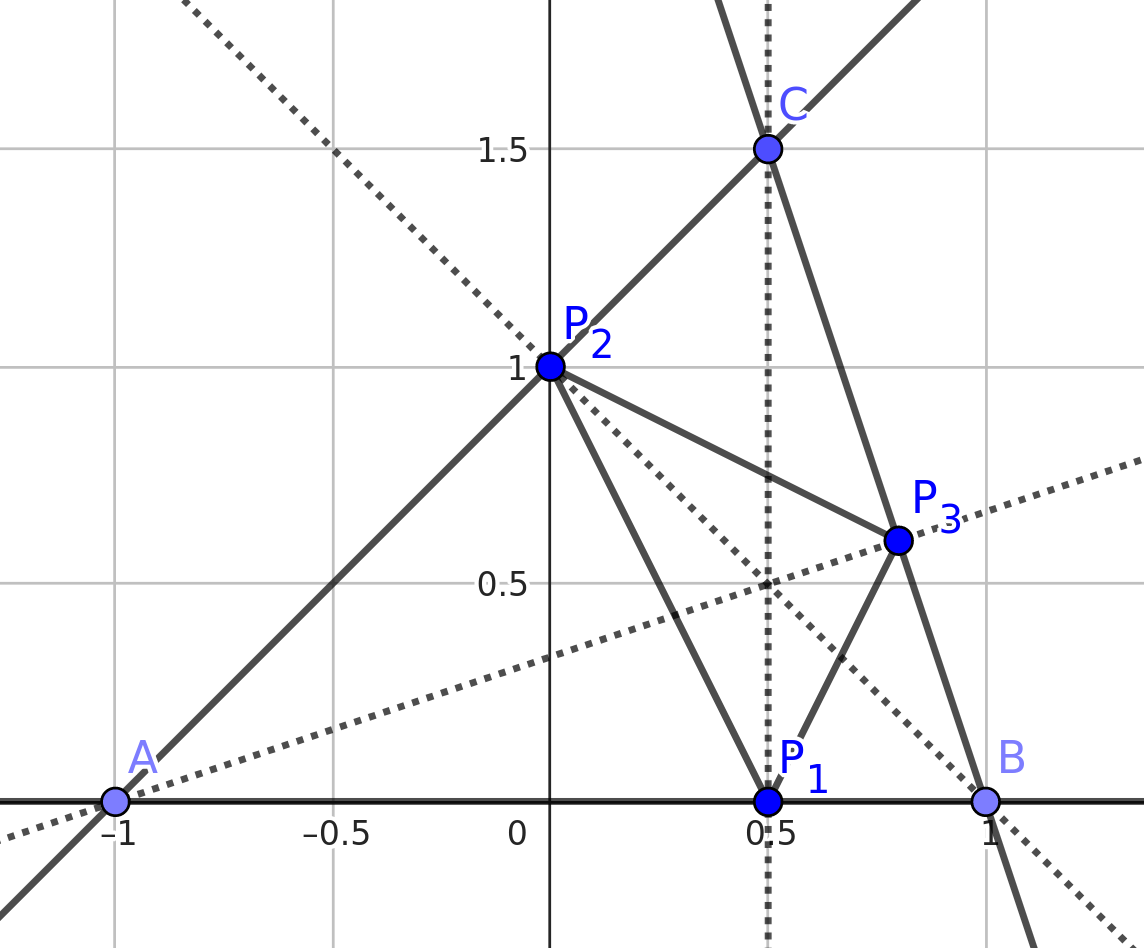
\includegraphics[width=0.9\textwidth]{geogebra_setup.png}
    \caption{A triangle with its orthic triangle drawn.}\label{fig:orthic_setup}
  \end{subfigure}%
  \begin{subfigure}{0.6\textwidth}
    \centering
    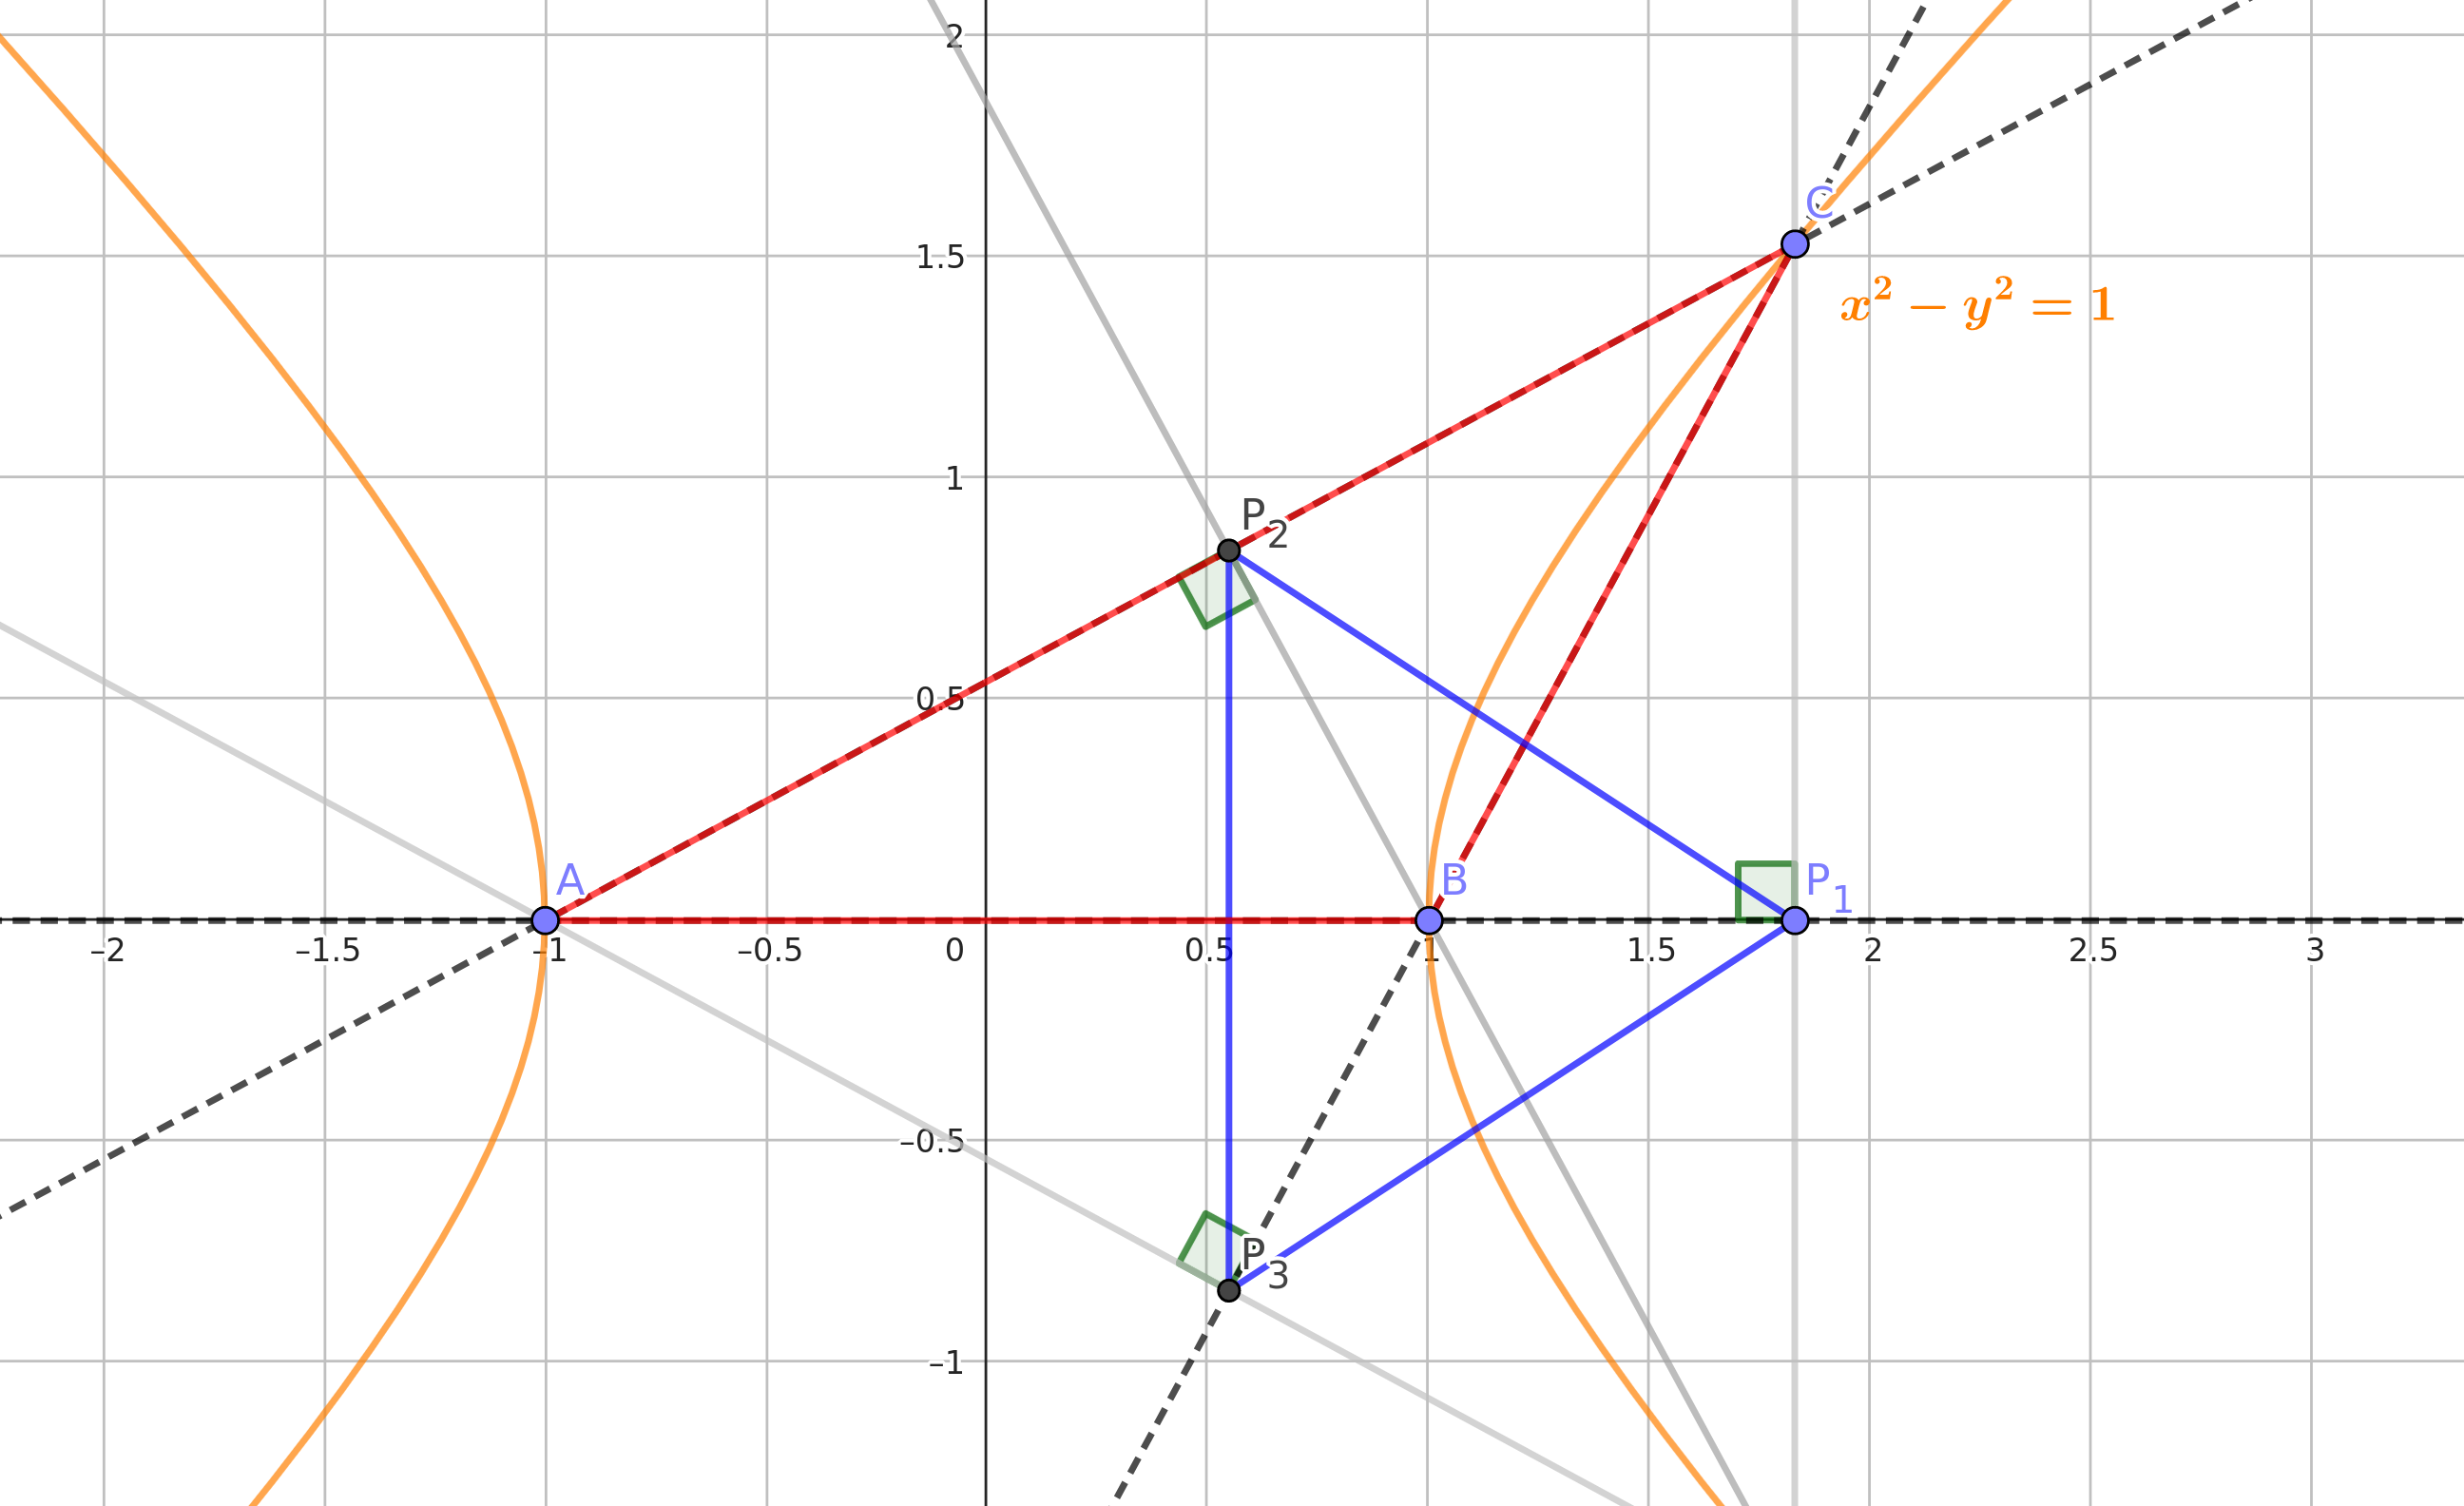
\includegraphics[width=0.9\textwidth]{geogebra_orthic.png}
    \caption{A triangle with a non-obvious isosceles orthic triangle.}\label{fig:orthic_solution}
  \end{subfigure}
  \caption{Orthic triangles}\label{fig:orthic}
\end{figure}

\begin{example}\label{ex:quant_elim}\upshape
  Consider a triangle with vertices $A = (-1, 0)$, $B = (1, 0)$ and $C = (a, b)$. Now, draw the three altitudes of the triangle $ABC$, and label their basepoints $P_{1} = (x_{1}, y_{1})$, $P_{2} = (x_{2}, y_{2})$ and $P_{3} = (x_{3}, y_{3})$, see figure~\ref{fig:orthic_setup}. The triangle $P_{1}P_{2}P_{3}$ is called the \textit{orthic} triangle of $ABC$. We wish to determine when the orthic triangle is isosceles with $|P_{1}P_{2}| = |P_{1}P_{3}|$. In other words, for which values of $a$ and $b$ does there exist points $P_{1} = (x_{1}, y_{1}), P_{2} = (x_{2}, y_{2}), P_{3} = (x_{3}, y_{3})$ such that those points are vertices of the orthic triangle, and $|P_{1}P_{2}| = |P_{1}P_{3}|$. Here, $AB$ denotes the vector pointing from point $A$ to point $B$ and $|AB|$ denotes its length.

  To solve this problem, we produce a parametric ideal that describes the setup. First, observe that $x_{1} = a$ and $y_{1} = 0$, so we make that substitution immediately. This also ensures that the line $CP_{1}$ is orthogonal to the line $AB$. Next, we need that the line $BP_{2}$ is orthogonal to the line $AC$. This means $0 = BP_{2} \cdot AC = (a + 1)(x_{2} - 1) + b y_{2}$. Similarly, to ensure that $AP_{3}$ is orthogonal to $BC$, we have $0 = (a - 1)(x_{3} + 1) + b y_{3}$. We also need to ensure that the points $P_{2}$ and $P_{3}$ lies on the edges of the triangle. This is done by forcing $0 = b(x_{2} + 1) - (a + 1)y_{2}$ and similarly $0 = b(x_{3} - 1) - (a - 1)y_{3}$. Finally, we need that $|P_{1}P_{2}| = |P_{1}P_{3}|$, which means that $0 = {(x_{3} - a)}^{2} + y_{3}^{2} - ({(x_{2} - a)}^{2} + y_{2}^{2})$. Hence, the following ideal describes the setup:
  \begin{align*}
    I = \langle\; &(a + 1)(x_{2} - 1) + b y_{2}, \quad  b(x_{2} + 1) - (a + 1)y_{2}, \\
                  &(a - 1)(x_{3} + 1) + b y_{3}, \quad  b(x_{3} - 1) - (a - 1)y_{3}, \\
                  & {(x_{3} - a)}^{2} + y_{3}^{2} - ({(x_{2} - a)}^{2} + y_{2}^{2}) \; \rangle
  \end{align*}

  If you want to follow along with the code, here is the code to compute a comprehensive parametric Gröbner basis:
  \begin{minted}{julia}
    using Nemo
    using ParametricGrobnerBases
    R, (a, b) = QQ[:a, :b]
    S, (x2, x3, y2, y3) = R[:x2, :x3, :y2, :y3]
    I = [(a + 1)*(x2 - 1) + b*y2, b*(x2 + 1) - (a + 1)*y2, (a - 1)*(x3 + 1) + b*y3, b*(x3 - 1) - (a - 1)*y3, (x3 - a)^2 + y3 - (x2 - a)^2 - y2^2]
    G = CGB(I)
  \end{minted}

  The result is a comprehensive parametric Gröbner basis $G$. It is too large to reproduce here, but can be found in appendix~\ref{app:CGB}. We see that the first element of the comprehensive parametric Gröbner basis is $a^{5} - 2a^{3} - ab^{4} + a$, which is only a constant term. Hence, it constrains us the most, since that constant term has to be 0. Note, that
  \[a^{5} - 2a^{3} - ab^{4} + a = a (a^{2} - b^{2} - 1) (a^{2} + b^{2} - 1) \]
  Since $\C$ is an integral domain, the product is zero if and only if at least one of the factors are zero. Thus, we have three cases:
  \begin{enumerate}
    \item $a = 0$ means that the triangle $ABC$ is isosceles. This immediately gives that $x_{3} = -x_{2}$ and $y_{2} = y_{3}$, which indeed gives us that $|P_{1}P_{2}| = |P_{1}P_{3}|$.
    \item $a^{2} + b^{2} - 1 = 0$. In this case, the triangle has a right angle in vertex $C$, which implies that $P_{2} = P_{3} = C$. Hence, $|P_{1}P_{2}| = |P_{1}P_{3}|$.
    \item $a^{2} - b^{2} - 1 = 0$. This equation traces out a hyperbola, and gives a surprising solution to the problem. Here, the orthic triangle does not sit inside the triangle $ABC$, and the points $P_{1}, P_{2}$ and $P_{3}$ might not be between the vertices. Instead, they lie on the infinite lines described by the vertices. See figure~\ref{fig:orthic_solution}.
  \end{enumerate}
  By carefully inspecting every other element of $\,G$, we see that if $\,b \neq 0$, i.e.\ the triangle is not degenerate, then every other element will have a non-zero non-constant term. Hence, the above gives us all solutions to the problem.
\end{example}

















\subsection{Parametric ideal membership \& pseudo-division}\label{sec:ps_div_app}
We can exploit lemma~\ref{lem:ps_rem_unique} to decide membership problems for parametric ideals.

\begin{theorem}
  Let $\,k_{1} \supset k$ be a field extension, let $\,I \subset k[U][X]$ be an ideal, and let $\mathcal G = \{(Y_{1}, G_{1}, \dots, (Y_{n}, G_{n}))\}$ be a comprehensive, reduced Gröbner system for $I$. Let $f \in k[U][X]$ and $\alpha \in k_{1}^{|U|}$, then $\sigma_{\alpha}(f) \in \langle \sigma_{\alpha}(I) \rangle$ if and only if there is an $i$ such that $\alpha \in Y_{i}$ and $\sigma_{\alpha}(r) = 0$, where $r$ is a pseudo-remainder of $f$ modulo $G_{i}$.
\end{theorem}
\begin{proof}
  Fix an $\alpha \in k_{1}^{|U|}$, and find some $i$ such that $\alpha \in Y_{i}$. This exists since $\mathcal G$ is comprehensive. Let $G_{i} = \{g_{1}, \dots, g_{m}\}$ and let
  \[c f = r + \sum_{j=1}^{m} h_{j} g_{j}\]
  be a pseudo-reduction. Then $\sigma_{\alpha}(f) \in \langle \sigma_{\alpha}(G_{i}) \rangle = \langle \sigma_{\alpha}(I) \rangle$ if and only if $\sigma_{\alpha}(r) = 0$, by lemma~\ref{lem:ps_rem_unique}.
\end{proof}

In this manner, we can determine conditions on when $\sigma_{\alpha}(f) \in \langle \sigma_{\alpha}(I) \rangle$. We simply require $\sigma_{\alpha}(r) = 0$, i.e. $\alpha \in Y_{i} \cap \V(r)$. Do note, that we might need to repeat this for each $Y$ with $\alpha \in Y$.

It is well-known, that standard geometric theorems can be expressed as memberships of polynomial ideals. For example, consider a triangle with vertices $A = (0, 0)$, $B = (x_{1}, y_{1})$ and $C = (x_{2}, y_{2})$. Then expressing that the triangle $ABC$ has a right angle in $A$ corresponds to $x_{1} x_{2} + y_{1} y_{2} = 0$. The pythagorean theorem $a^{2} + b^{2} = c^{2}$ corresponds to $x_{1}^{2} + y_{1}^{2} + x_{2}^{2} + y_{2}^{2} = {(x_{1} - x_{2})}^{2} + {(y_{1} - y_{2})}^{2}$. In algebraic terms, the fact that the pythagorean theorem holds for right triangles, is the statement that
\[x_{1}^{2} + y_{1}^{2} + x_{2}^{2} + y_{2}^{2} - \left({(x_{1} - x_{2})}^{2} + {(y_{1} - y_{2})}^{2}\right) \in \sqrt{\langle x_{1} x_{2} + y_{1} y_{2} \rangle} \]
In general, a geometric conclusion $f \in k[X]$ follows from a set of assumptions generating the ideal $I$ if and only if $f \in \sqrt{I}$. Here, $\sqrt{I}$ is the radical of $I$, given by $\sqrt{I} = \{f \in k[X] \mid \exists n \in \N : f^{n} \in I\}$. Thankfully, $\sqrt{ \langle x_{1} x_{2} + y_{1} y_{2} \rangle } = \langle x_{1} x_{2} + y_{1} y_{2} \rangle$. However, in general, computing the radical of an ideal is quite difficult. We do however have the following theorem.

\begin{theorem}\label{thm:rad}
  Let $I \subset k[X]$ be an ideal, and let $f \in k[X]$. Then $f \in \sqrt{I}$ if and only if $1 \in I + \langle 1 - yf \rangle \in k[X, y]$, where we have added a new variable. This can be checked using Gröbner bases.
\end{theorem}
\begin{proof}
  See chapter 3,  proposition 8 in~\cite{IVA}. Checking whether $1 \in I + \langle 1 - yf \rangle$ can be done by computing a Gröbner basis $G$ of $I + \langle 1 - yf \rangle$, then $1 \in I + \langle 1 - yf \rangle$ if and only if $G$ contains a unit.
\end{proof}

By computing reduced Gröbner systems, this gives a different way of discovering geometric theorems based on pseudo-remainders.

\begin{theorem}\label{thm:in_rad_iff_r_eq_z}
  Let $\,I \subset k[U][X]$ be an ideal, let $\,(Y, G)$ be a segment of a reduced Gröbner system for $I$ and let $f \in k[U][X]$. Assume that $r$ is a pseudo-remainder of $f$ modulo $G$ and that $r \in k[U]$. Then $\sigma_{\alpha}(f) \in \sqrt{\langle \sigma_{\alpha}(I) \rangle}$ if and only if $\sigma_{\alpha}(r) = 0$.
\end{theorem}
\begin{proof}
  If $\langle \sigma_{\alpha}(I) \rangle = \langle 1 \rangle$, then $\sqrt{\langle \sigma_{\alpha}(I) \rangle} = \langle \sigma_{\alpha}(I) \rangle$ so the conclusion follows from lemma~\ref{lem:ps_rem_unique}. Hence, we assume that $\langle \sigma_{\alpha}(I) \rangle \neq \langle 1 \rangle$.

  Let $r$ be a pseudo-remainder of $f$ modulo $G$. If $\sigma_{\alpha}(r) = 0$, then $\sigma_{\alpha}(f) \in \langle \sigma_{\alpha}(I) \rangle \subset \sqrt{\langle \sigma_{\alpha}(I) \rangle}$. On the other hand, if $\sigma_{\alpha}(f) \in \sqrt{\langle \sigma_{\alpha}(I) \rangle}$, then $\sigma_{\alpha}(r) \in \sqrt{\langle \sigma_{\alpha}(I) \rangle} $. Hence $1 \in \langle \sigma_{\alpha}(I) \rangle + \langle 1 - y \sigma_{\alpha}(r) \rangle$ by theorem~\ref{thm:rad}. Since $r \in k[U]$ we have $\sigma_{\alpha}(r) \in k$, and since $\langle \sigma_{\alpha}(I) \rangle \neq \langle 1 \rangle$, $\sigma_{\alpha}(G)$ does not contain a unit. As $\LM(1 - y \sigma_{\alpha}(r)) = y$ when $\sigma_{\alpha}(r) \neq 0$, every leading monomial in $G$ is relatively prime to $\LM(1 - y \sigma_{\alpha}(r))$. By a standard theorem, see proposition 4 in chapter 2 of~\cite{IVA}, this implies that $\sigma_{\alpha}(G) \cup \{1 - y \sigma_{\alpha}(r)\}$ is a Gröbner basis of $\langle \sigma_{\alpha}(I) \rangle + \langle 1 - y \sigma_{\alpha}(r) \rangle$. Hence, $1 \in \langle \sigma_{\alpha}(I) \rangle + \langle 1 - y \sigma_{\alpha}(r) \rangle$ if and only if $\sigma_{\alpha}(r) = 0$.
\end{proof}

Let us again take the example of the orthic triangle from~\cite{MONTES20101391}.


\begin{example} \upshape
  As in example~\ref{ex:quant_elim}, we consider the ideal
  \begin{align*}
    I = \langle\; &(a + 1)(x_{2} - 1) + b y_{2}, \quad  b(x_{2} + 1) - (a + 1)y_{2}, \\
                  &(a - 1)(x_{3} + 1) + b y_{3}, \quad  b(x_{3} - 1) - (a - 1)y_{3} \; \rangle
  \end{align*}
  but this time without the polynomial representing the conclusion. Instead we let the conclusion polynomial
  \[f = (x_{3} - 1)^{2} + y_{3}^{2} - (x_{2} - a) - y_{2}^{2}\]
  be seperate, and ask when $\sigma(f) \in \sqrt{\langle \sigma(I) \rangle}$. In Julia, the setup is as follows:

  \begin{minted}{julia}
    using Nemo
    using ParametricGrobnerBases
    R, (a, b) = QQ[:a, :b]
    S, (x2, x3, y2, y3) = R[:x2, :x3, :y2, :y3]
    I = [(a + 1)*(x2 - 1) + b*y2, b*(x2 + 1) - (a + 1)*y2, (a - 1)*(x3 + 1) + b*y3, b*(x3 - 1) - (a - 1)*y3]
    f = (x3 - a)^2 + y3^2 - (x2 - a)^2 - y2^2
    CGS(I)
  \end{minted}

  To answer the question, we can use the output of $\mathbf{CGS}(I)$. It returns several segments, but most of them has the condition $b = 0$, leading to a degenerate triangle. There is only one case, which is interesting:

  \[(V(0) \setminus \V((a^{2} + 2a + b^{2} + 1)(a^{2} - 2a + b^{2} + 1)b)\;, \; G )\] where
  \begin{align*}
 G = \{\; &(a^2 - 2a + b^2 + 1)y_3 + 2ab - 2b \\
          &(a^2 + 2a + b^2 + 1)y_2 - 2ab - 2b \\
          &(a^2b - 2ab + b^3 + b)x_3 + a^2b - 2ab - b^3 + b \\
          &(a^2b + 2ab + b^3 + b)x_2 - a^2b - 2ab + b^3 - b \; \}
  \end{align*}

  The condition states that $\sigma(b) \neq 0$. The polynomials $a^{2} + 2a + b^{2} + 1$ and $a^{2} - 2a + b^{2} + 1$ has only the real roots $(a, b) = (-1, 0)$ and $(a, b) = (1, 0)$ respectively. Hence, on the real plane, the condition only states that $\sigma(b) \neq 0$.

  To determine whether $f$ lies in this segment, we compute a pseudo-remainder of $f$ modulo $G$. Like this in Julia:

  \begin{minted}{julia}
    G = CGS(I)[1][3]
    r = pseudo_reduce(f, G)[2]
    factor(r)
  \end{minted}
  This gives
  \begin{align*}
    r = &4 a^{17} b^4 + 24 a^{15} b^6 - 32 a^{15} b^4 + 56 a^{13} b^8 - 120 a^{13} b^6 + 112 a^{13} b^4 + 56 a^{11} b^{10} - \\
        &144 a^{11} b^8 + 216 a^{11} b^6 - 224 a^{11} b^4 - 40 a^9 b^{10} + 72 a^9 b^8 - 120 a^9 b^6 + 280 a^9 b^4 - \\
        &56 a^7 b^{14} - 16 a^7 b^{10} + 32 a^7 b^8 - 120 a^7 b^6 - 224 a^7 b^4 - 56 a^5 b^{16} - 72 a^5 b^{14} - \\
        &16 a^5 b^{10} + 72 a^5 b^8 + 216 a^5 b^6 + 112 a^5 b^4 - 24 a^3 b^{18} - 80 a^3 b^{16} - 72 a^3 b^{14} - \\
        &40 a^3 b^{10} - 144 a^3 b^8 - 120 a^3 b^6 - 32 a^3 b^4 - 4 a b^{20} - 24 a b^{18} - 56 a b^{16} - 56 a b^{14} + \\
        &56 a b^{10} + 56 a b^8 + 24 a b^6 + 4 a b^4 \\
    = &4 b^{4}\cdot {(a^{2} + 2a + b^{2} + 1)}^{3} \cdot {(a^{2} - 2a + b^{2} + 1)}^{3} \cdot a \cdot (a^{2} - b^{2} - 1) \cdot (a^{2} + b^{2} - 1)
  \end{align*}

  Since $\sigma(f) \in \sqrt{\langle \sigma(I) \rangle}$ if and only if $\sigma(r) = 0$ by theorem~\ref{thm:in_rad_iff_r_eq_z}, we just need to find values of $a$ and $b$, that set $r$ to zero. By considering the factorization, we have five factors we can make 0, in order to get $r$ to be 0. However, neither $a^{2} + 2a + b^{2} + 1$, $a^{2} - 2a + b^{2} + 1$ nor $b$ can be $0$ by the conditions on the segment. So, we're left with the same three options as in example~\ref{ex:quant_elim}.

  We also get that for every other value of $a$ and $b$, we have $\sigma(r) \neq 0$ since $\C$ is an integral domain. Hence $\sigma(f) \notin \sqrt{\langle \sigma(I) \rangle}$, meaning that the triangle does not have an isosceles orthic triangle. In this way, we have found nescessary and sufficient conditions for the geometric theorem.
\end{example}

It should be noted, that even though the conclusion is exactly the same as in example~\ref{ex:quant_elim}, the method is completely different. Is has two main advantages: first, we can reuse the Gröbner system, independently of the conclusion. In other words, if instead we wanted to ask whether a side of the orthic triangle was parallel to a side of $ABC$, we can do that immediately from $G$ using pseudo-divisions\footnote{The answer is rather boring: it never happens for a non-degenerate triangle.}. In the other approach, we would need to recompute the parametric Gröbner basis, which may well take a long time for more complex applications. Secondly, we only have a single polynomial, namely the pseudo-remainder, to consider instead of having to take the entire Gröbner basis into acount. This leads to a test, which is easier to automate.

The method described above does have a drawback, which is the added assumption on the pseudo-remainder. We assumed, that the pseudo-remainder $r$ is an element of $k[U]$. Of course, that does not always happen. It is, however, a reasonable assumption, for the following reason. If $k$ is algebraically closed and the points $x_{1}, \dots, x_{n}$ are uniquely determined by the parameters on a segment $(Y, G)$, then $\LM(G) = \{x_{1}, \dots, x_{n}\}$. This is because, when $k$ is algebraically closed, the only solution will then correspond to a maximal ideal. Since no term of the pseudo-remainder $r$ is divisible by any element of $\LM(G)$, this implies that $r \in k[U]$.

Notice, how all of the above has assumed that $k$ is algebraically closed. This means, that the method might not be usable in the real plane. Let us take one more example, to illustrate why this approach works better in the complex plane than the real plane.

\begin{example}\upshape
  Let $I$ and $G$ be given as before. We want to answer when the area of the orthic triangle is one fifth of the area of the whole triangle. The area of the triangle $ABC$ is $A_{ABC} = b$, and by using the shoelace formula we find that the area of the orthic triangle is $A_{o} = \frac{1}{2}(a(y_{2} - y_{3}) + x_{2} y_{3} - x_{3} y_{2})$. However, those are signed areas, so if the triangle is five times as large as its orthic triangle, we can either have $A_{ABC} = 5 A_{o}$ or $A_{ABC} = -5 A_{o}$. Hence, the polynomial representing the conclusion is $f = (A_{ABC} - 5 A_{o})(A_{ABC} + 5 A_{o})$, since $\sigma(f) = 0$ if and only if either $A_{ABC} = 5 A_{o}$ or $A_{ABC} = -5 A_{o}$. After pseudo-reducing $f$ by $G$, we get a pseudo-remainder that is too large to reproduce, but its factorization is
  \begin{align*}
    r = &-b^{7} \cdot {(a^{2} + b^{2} - 2a + 1)}^{11} \cdot {(a^{2} + b^{2} + 2a + 1)}^{8} \cdot \\
        &(11a^{4} + 12a^{2}b^{2} + b^{4} - 22a^{2} - 8b^{2} + 11) \cdot (9a^{4} + 8a^{2}b^{2} - b^{4} - 18a^{2} - 12b^{2} + 9)
  \end{align*}

  We see that $\sigma(f) \in \sqrt{\langle \sigma(I) \rangle}$ if and only if $\sigma(11a^{4} + 12a^{2}b^{2} + b^{4} - 22a^{2} - 8b^{2} + 11) = 0$ or $\sigma(9a^{4} + 8a^{2}b^{2} - b^{4} - 18a^{2} - 12b^{2} + 9) = 0$. We'll focus on the first condition. In the complex plane, this is fine. The polynomial is quartic in both $a$ and $b$, so for every fixed value of $a$, we get four solutions for $b$, counted with multiplicity. The real case, however, is not as simple.

  Using a CAS system we get the following roots of the polynomial:
  \[b = \pm \sqrt{4 - 6 a^2 \pm \sqrt{5 - 26 a^2 + 25 a^4}}\]
  We can plot one of the inner functions:

  \begin{center}
    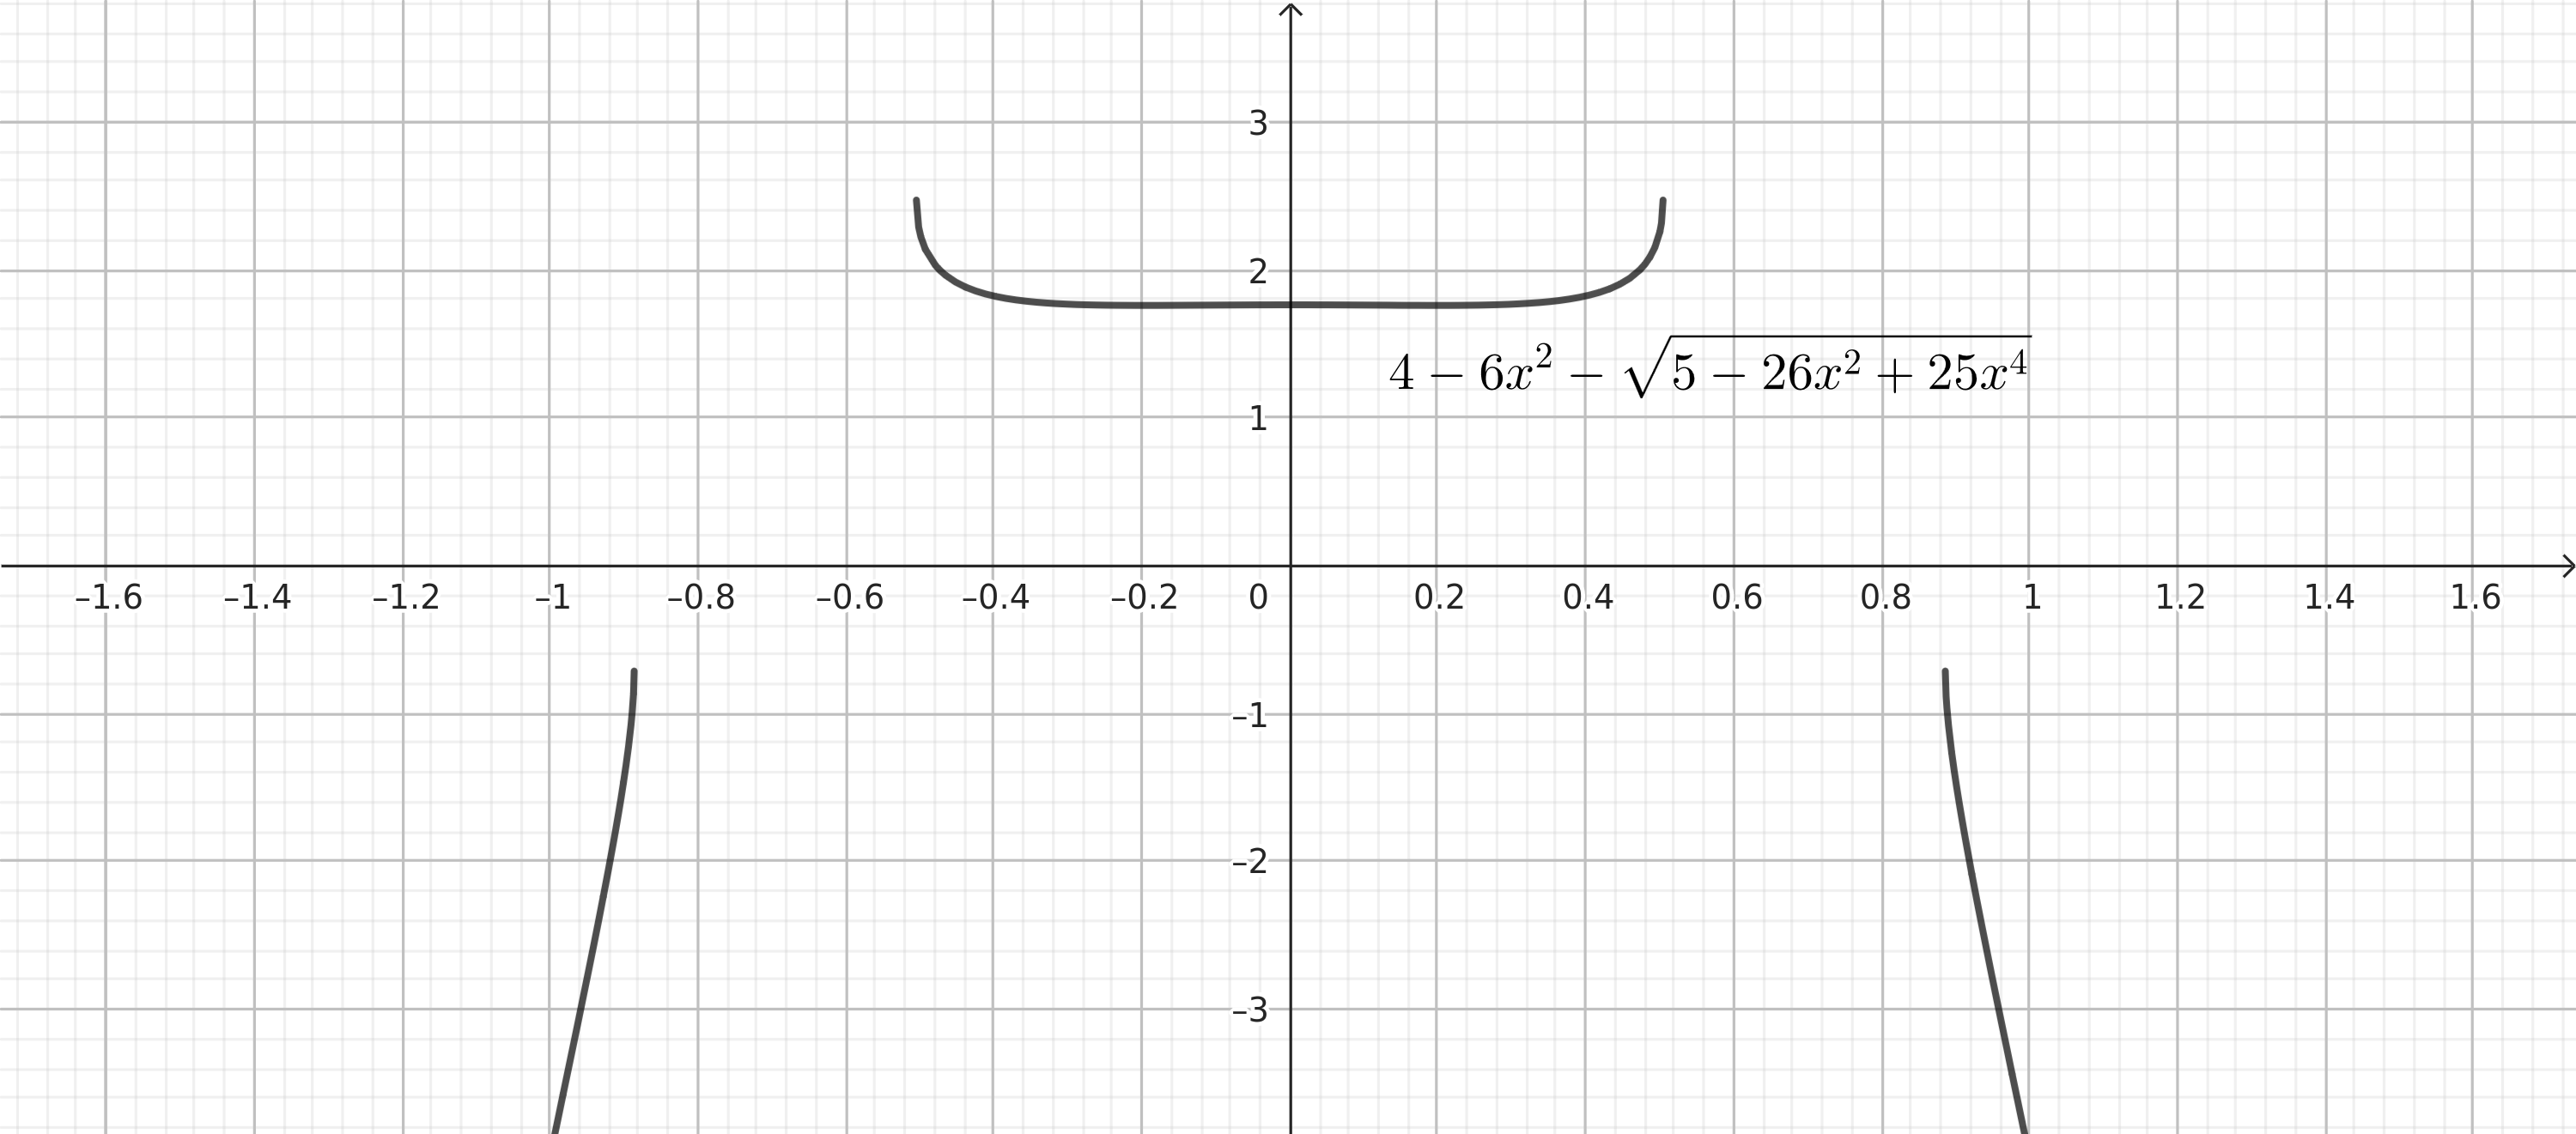
\includegraphics[width=0.7\textwidth]{geogebra_sqrt.png}
  \end{center}
  This shows us, that when $a$ lies between $-0.51$ and $0.51$, the polynomial above has a solution in the real plane. By looking at the other branches of the solution, we see that there is also an isolated solution in $a = 1$, $b = 0$ corresponding to the degenerate triangle. However, this solution is excluded by the conditions on the segment. For other values of $a$ there is no solution over the reals.

  By doing a bit of manual analysis and plotting parts of the graph seperately, the complete set of solutions in the real plane can be found on figure~\ref{fig:orthic_wow}. The two ``blobs'' are solutions for acute triangles, whereas the the two unbounded curves correspond to solutions for obtuse triangles.

  We're lucky in this case, as the quartic is solvable in radicals. Had the pseudo-remainder been of fifth degree (ignoring the factors from the conditions on the segment), we might not be able to say much about the real case. Furthermore, even though the points $x_{1}, \dots, x_{n}$ are uniquely determined, and hence $\langle \sigma(I) \rangle$ is a maximal ideal, that may not imply that $\LM(G) = \{x_{1}, \dots, x_{n}\}$. In that case, we're not guaranteed that the pseudo-remainder only contains parameters.

  Hence this method of discovering geometric theorems may not always work in the real plane. It could, however, be a useful first step, as we do get nescesary and sufficient conditions for the theorem to be true. Those conditions just might be difficult to analyse, but more sophisticated tools can use this as a first step, see~\cite{10.1145/2755996.2756646}.

  % Further experimentation reveals, that for acute triangles, the the area of the orthic triangle can reach a maximum of one fourth of $A_{ABC}$. For obtuse triangles, it seems like the orthic triangle can get almost twice as big as $ABC$, but not quite. This also highlights another limitation of this approach, that we're only able to answer questions, which can be encoded as a polynomial. Determining which triangles has be largest ratio between the areas of the triangle and its orthic triangle is not possible with this technique. Although, using numeric optimization techniques, one could get reasonable answer.
\end{example}

\begin{figure}[t]
  \begin{center}
    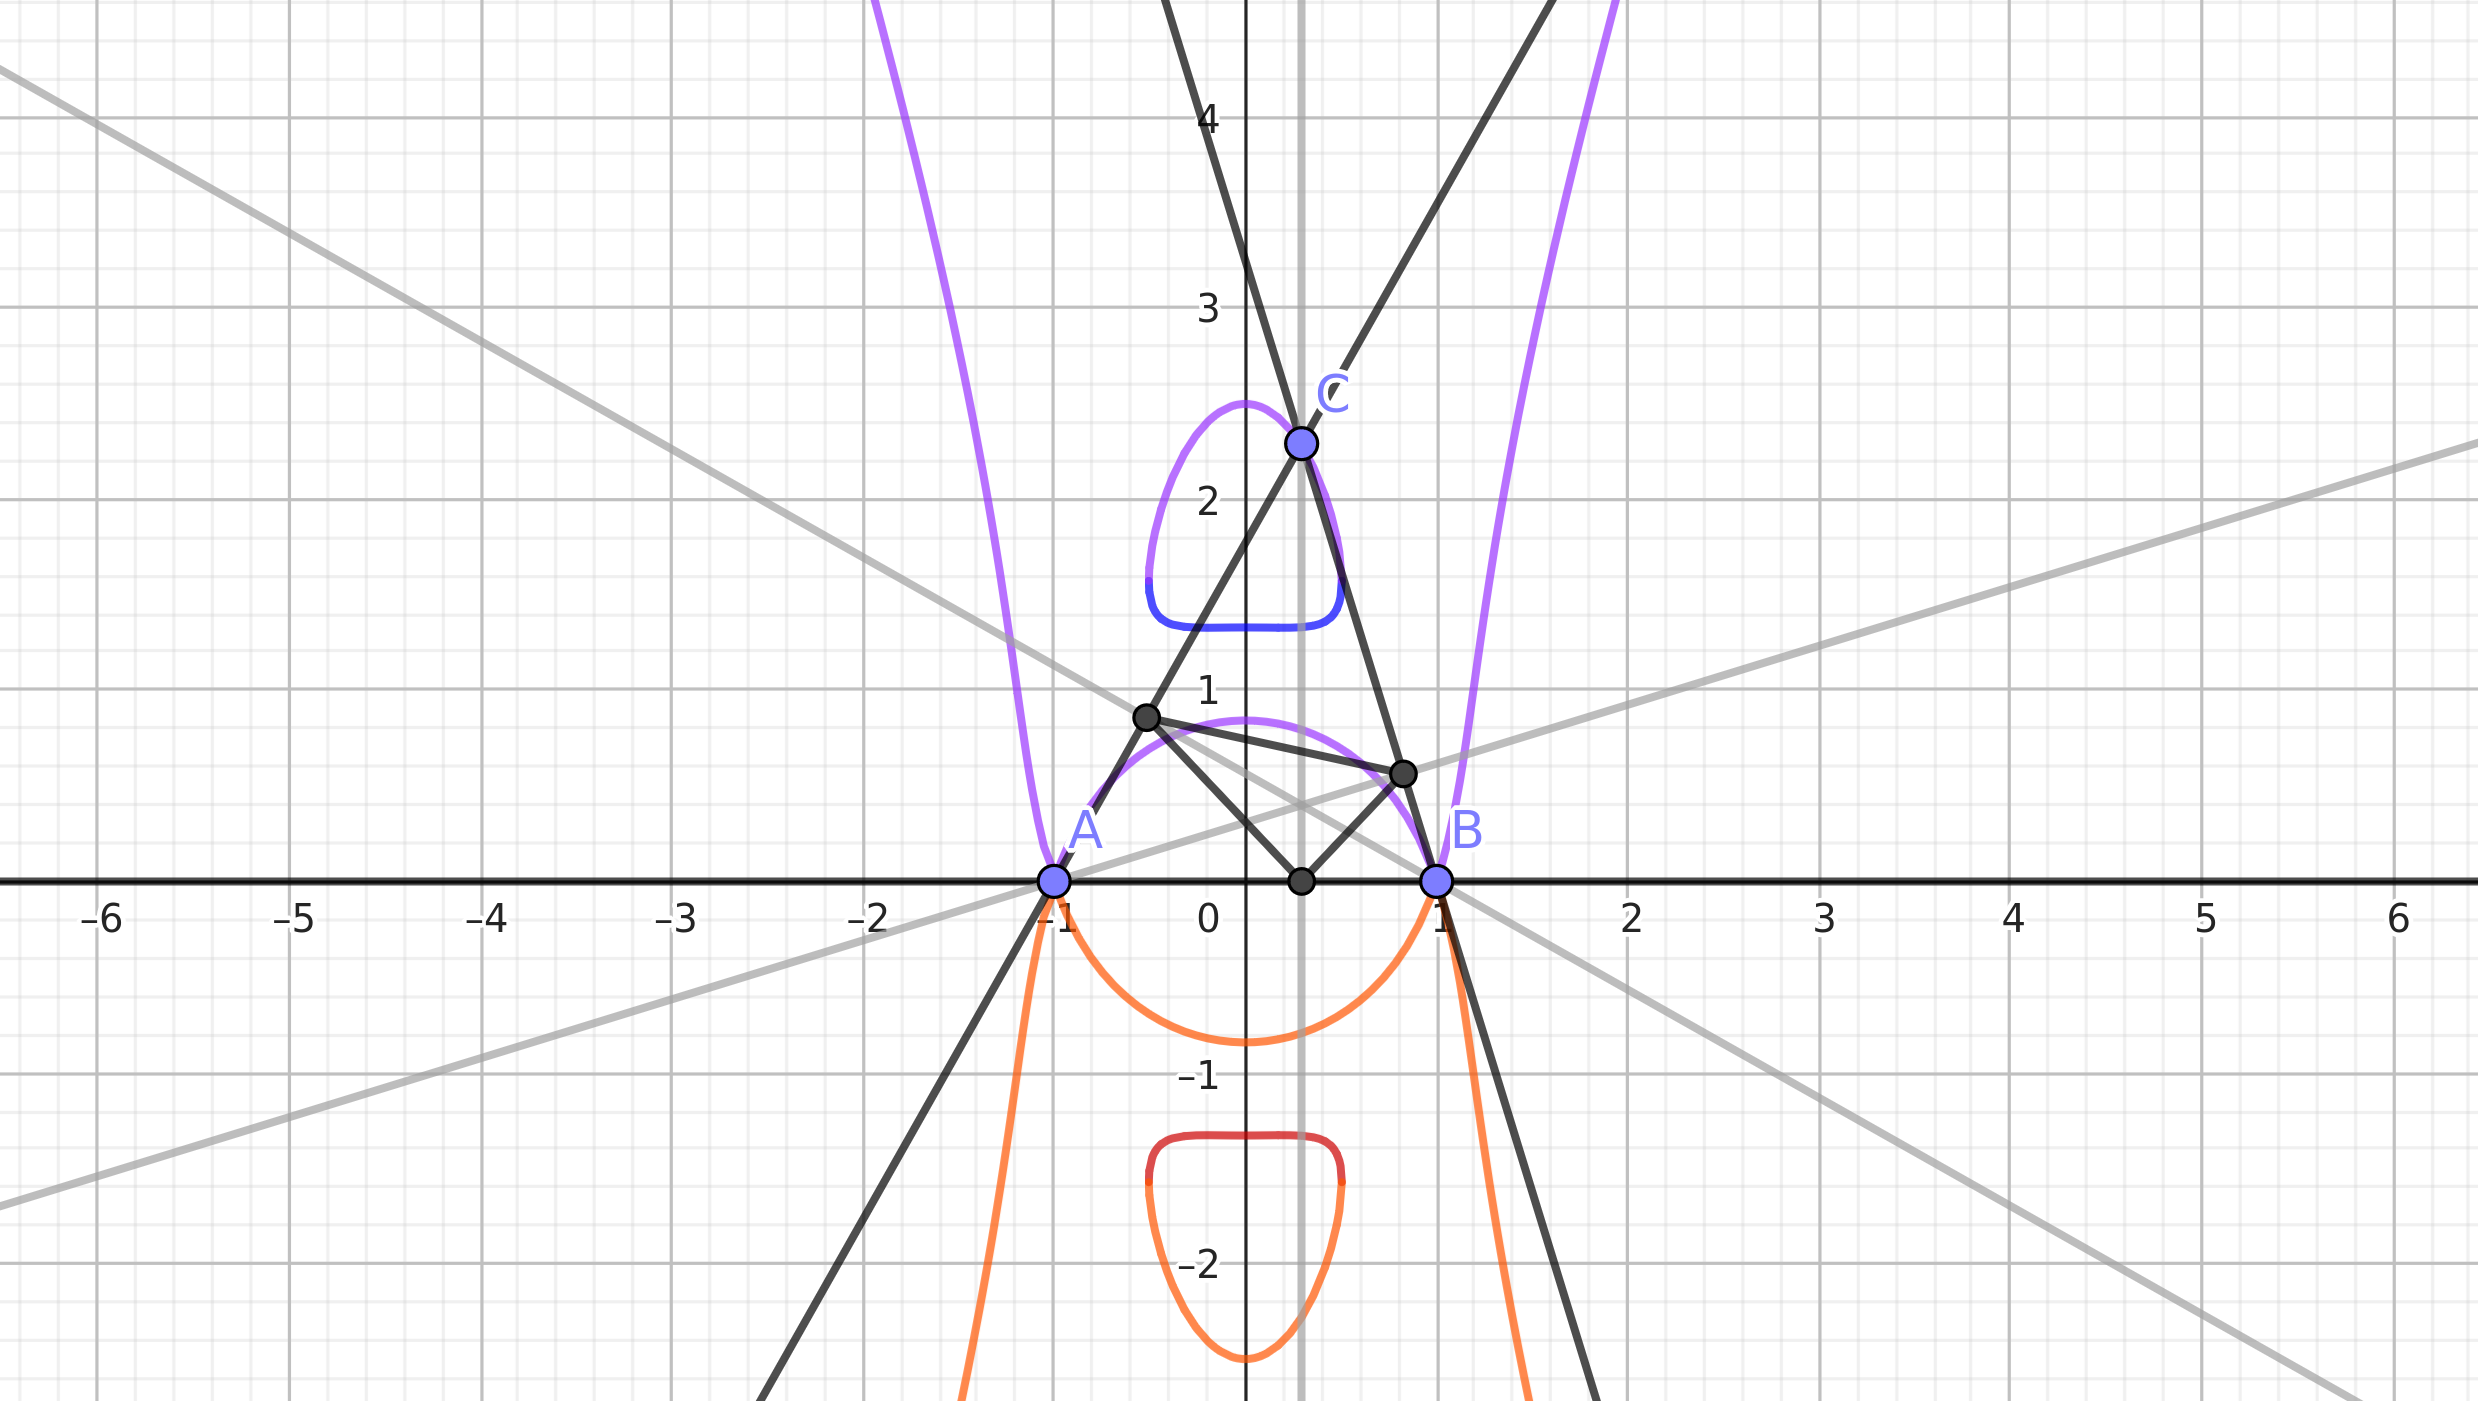
\includegraphics[width=0.7\textwidth]{geogebra_orthic_wow2.png}
  \end{center}
  \caption{The set of real points, where the area of the orthic triangle is exactly one fifth of the area of the triangle $ABC$}\label{fig:orthic_wow}
\end{figure}










\subsection[Bernds conjecture]{Bernds conjecture\footnote{Named such by Bernd Sturmfels in a private communication to the supervisor of this project.}}\label{sec:bernd}
In the article~\cite{sturmfels}, Bernd Sturmfels states the following theorem without proof.

\begin{theorem}
  Let $K$ be an algebraically closed field and $F = \{f_{1}, \dots, f_{k}\} \subset K[x_{1}, \dots, x_{n}]$ a finite set of polynomials. Assume that $\,\V(F) = \emptyset$ and consider the ideal $\,I = \langle y_{1} - f_{1}, \dots, y_{k} - f_{k} \rangle \subset K[x_{1}, \dots, x_{n}, y_{1}, \dots, y_{k}]$. Let $G$ be a Gröbner basis of $\,I$ with respect to the lexicographic order with $x_{1} > \cdots > x_{n} > y_{1} > \cdots > y_{k}$. Then $G$ contains a polynomial $p$ (called a final polynomial) such that
  \begin{enumerate}
    \item $p(x_{1}, \dots, x_{n}, 0, 0, \dots, 0) \in K \setminus \{0\}$
    \item $p(x_{1}, \dots, x_{n}, f_{1}, \dots, f_{k}) = 0$.
  \end{enumerate}
\end{theorem}

He writes that the proof is ``straightforward but fairly technical''. In a private communication\cite{NL_to_BS} with Sturmfels, he encourages us to write a proof or find a counterexample. He also writes, that the gist of the argument he had in mind was using specializations of Gröbner bases. Since $\{x_{1}, \dots, x_{n}\} \gg \{y_{1}, \dots, y_{k}\}$, the Gröbner basis of $I$ would specialize to a Gröbner basis of $\langle F \rangle$ when we specialize the $y_{i}$'s to zero. However, as we have seen, Gröbner bases can be most unstable under specializations. Indeed, the following counterexample disproves this line of reasoning and the theorem.

\begin{example}\upshape
  Let $F = \{f_{1}, f_{2}\}$ where $f_{1} = x_{1} x_{2} + 1$ and $f_{2} = x_{2}$. Then, the corresponding ideal
  $I = \langle y_{1} - f_{1}, y_{2} - f_{2} \rangle$ has the following reduced Gröbner basis w.r.t.\ the lexicographic order with $x_{1} > x_{2} > y_{1} > y_{2}$: $G =  \{g_{1}, g_{2}\}$ where $g_{1} = x_{2} - y_{2}$ and $ g_{2} = y_{2}x_{1} - y_{1} + 1$. Consider now $G' = \{g_{1}, g_{1} - g_{2}\} = \{x_{2} - y_{2}, y_{2}x_{1} + x_{2} - y_{1} - y_{2} + 1\}$. Clearly $\langle G' \rangle = \langle G \rangle = I$, and it is still a Gröbner basis since $\LT(G') = \LT(G)$. However, letting $\sigma$ be the specialization setting $\sigma(y_{1}) = \sigma(y_{2}) = 0$, we see that
  \[\sigma(G') = \{x_{2}, 1+x_{2}\}\]
  which is not a Gröbner basis. Furthermore, we see that $G'$ does not contain a final polynomial.
\end{example}

While this example is admittedly a bit contrived, the theorem is false, even if we require the Gröbner basis to be reduced.

\begin{example}\upshape
    Let $F = \{f_1, f_2, f_3\}$ where $f_1 = x_2 + x_3$, $f_2 = x_2 x_3$ and $f_3 = x_1 x_3 + 1$. The reduced Gröbner basis of $\langle F \rangle$ is $\{1\}$, so $F$ has no common zeros. The corresponding ideal $I = \langle y_1 - f_1, y_2 - f_2, y_3 - f_3 \rangle$ has the reduced Gröbner basis
    \begin{gather*}
    G = \{ x_3^2 - x_3 y_1 + y_2, x_2 + x_3 - y_1, x_1 y_2 + x_3 y_3 - x_3 - y_1 y_3 + y_1, x_1 x_3 - y_3 + 1\}.
    \end{gather*}
    When specializing $y_1 = y_2 = y_3 = 0$, $G$ turns into
    \[\bar G = \{ x_3^2, x_2 + x_3, -x_3, x_1 x_3 + 1\}\]
    which is not a Gröbner basis, and does not contain a constant. Hence, $G$ does not contain a final polynomial.
\end{example}

To fix the theorem, we can turn to parametric Gröbner bases. To shorten notation, let $X = \{x_{1}, \dots, x_{n}\}$ and $Y = \{y_{1}, \dots, y_{k}\}$.

\begin{theorem}
  Let $K$ be an algebraically closed field and let $F = \{f_{1}, \dots, f_{k}\} \subset K[X]$ be a finite set of polynomials. Assume that $\V(F) = \emptyset$ and consider the ideal $I = \langle y_{1} - f_{1}, \dots, y_{k} - f_{k} \rangle \subset K[X, Y]$. Let $G$ be a comprehensive parametric Gröbner basis of $\,I$ with respect to any monomial order. Then $G$ contains a final polynomial.
\end{theorem}
\begin{proof}
  First, notice that every polynomial in $I$ satisfies the second property of final polynomials, since the generators does, and the evaluation map is linear. Thus, we only need to prove that a parametric Gröbner basis contains an element satisfying the first property.

  Let $G$ be a parametric Gröbner basis of $I$, and let $\sigma$ be the specialization setting $\sigma(y_{i}) = 0$ for every $i$. Since $\langle \sigma(I) \rangle = \langle F \rangle = \langle 1 \rangle$, there must be some element $g \in G$ where $\LM(\sigma(g)) \mid 1$, implying that $g$ is a final polynomial.
\end{proof}

However, parametric Gröbner bases can be quite expensive to compute since we need to repeatedly compute Gröbner bases, and furthermore we don't have nice bounds on the degrees. But we only care about one single specialization. This means we don't need a parametric Gröbner basis, we just need a faithful segment of a Gröbner system covering the origin. Here, we can use lemma~\ref{lem:grb_if_nmap_to_z_t}. Let $\sigma^{1} : K[t, X, Y] \to K[X, Y]$ be the map evaluating $t$ to 1, and let $\sigma^{0} : K[t, X, Y] \to K[X, Y]$ be the map evaluating $t$ to 0.

\begin{theorem}
  Let $K$ be an algebraically closed field and $F = \{f_{1}, \dots, f_{k}\} \subset K[X]$ a finite set of polynomials. Assume that $\V(F) = \emptyset$ and consider the ideal $I = \langle \hat F \rangle$ where $\hat F = \{y_{1} - f_{1}, \dots, y_{k} - f_{k}\}$. Now, let $\,G$ be the reduced Gröbner basis of the ideal $\langle t \cdot \hat F \cup (1 - t) \cdot Y \rangle \subset K[t, X, Y]$ w.r.t.\ any monomial order with $t \gg X \gg Y$. Then $\sigma^{1}(G)$ contains a final polynomial.
\end{theorem}
\begin{proof}
  As before, we only need to show that $\sigma^{1}(G)$ contains a polynomial satisfying the first property of final polynomials. Let $\sigma : K[X, Y] \to K[X]$ be the specialization setting $\sigma(y_{i}) = 0$ for every $i$ and let $H = \{\LC_{Y}(g) \mid g \in G, \LT(g) \notin K[X, Y], \LC_{X, Y}(g) \notin \langle Y \rangle\}$. If we have $0 \in \V(Y) \setminus \V(\lcm(H))$, then lemma~\ref{lem:grb_if_nmap_to_z_t} gives us that $\sigma(\sigma^{1}(G))$ is a Gröbner basis of $\langle \sigma(I) \rangle = \langle F \rangle$. By the Nullstellensatz, $\langle F \rangle = \langle 1 \rangle$, so $\sigma(\sigma^{1}(G))$ has to contain a constant. This implies, that $\sigma^{1}(G)$ contains a final polynomial $g$.

  Now, we just need that $0 \in \V(Y) \setminus \V(\lcm(H))$. Since $\V(Y) = \{0\}$, we just need that $\V(Y) \nsubset \V(\lcm(H))$. By lemma~\ref{lem:LC_U_notin_S} we have that $h \notin \langle Y \rangle$ for each $h \in H$. Since $\langle Y \rangle$ is a prime ideal, this implies that $\lcm(H) \notin \langle S \rangle$. Thus $\V(Y) \nsubset \V(\lcm(H))$.
\end{proof}

This counterexample and theorem was developed in colaboration with Peter Lundgaard, and resulted in an article~\cite{Lundgaard_Poulsen}. In that article, it is also proven that it is sufficient to compute a Gröbner basis of $\langle y_{1} - z f_{1}, \dots, y_{k} - z f_{k} \rangle$. However, that proof requires a little more care, whereas this proof follows directly from the theory of parametric Gröbner bases.

\newpage





\printbibliography


\appendix
\newpage
\section{Miscellaneous results}
In this section, we prove results that we need in the main text, but don't fit in the flow of the text. The last two are well-known results, which nevertheless aren't usually covered in introductory algebra courses. Hence, we present them here.

\subsection{The pseudo-division algorithm}\label{app:pseudo}
The pseudo-division algorithm is a slight modification of the normal division algorithm.

\begin{theorem}
  Let $f \in A[X]$ and $\,G = \{g_{1}, \dots, g_{n}\} \subset A[X]$. Then there exists $\,\{h_{1}, \dots, h_{n}\} \subset A[X]$, $r \in A[X]$ and $c \in A$ such that
  \[c f = r + \sum_{i=1}^{n} h_{i} g_{i}\]
  and the following properties are satisfied:
  \begin{enumerate}
    \item $c = \prod_{i=1}^{n} \LC(g_{i})^{p_{i}}$ for some powers $p_{i} \geq 0$.
    \item $\LM(h_{i} g_{i}) \leq \LM(f)$ for all $i \in \{1, \dots, n\}$.
    \item No term of $\,r$ is divisible by $\LM(g_{i})$ for any $i$,
    \item $\coef(h_{i} g_{i}, m) \in \langle \coef(f, m') \mid m' \geq m \rangle$ for all $i \in \{1, \dots, n\}$ and all monomials $m$.
  \end{enumerate}
\end{theorem}
\begin{proof}
  First, we present the division algorithm to compute such a representation. To start, let $f^{0} = f$, $r^{0} = 0$, $c^{0} = 1$ and $h_{1}^{0} = h_{2}^{0} = \dots = h_{n}^{0} = 0$. Then we iteratively define the state at step $i$ in terms of the state at step $i-1$:
  \begin{itemize}
    \item If $f^{i-1} = 0$, we are done. Set $r = r^{i-1}$, set $c = c^{i-1}$ and set $h_{j} = h_{j}^{i-1}$ for all $j \in \{1, \dots, n\}$.
    \item If there is some $g_{j} \in G$ such that $\LM(g_{j}) \mid \LM(f^{i-1})$, then find a monomial $\gamma$ such that $\LM(g_{j})\gamma = \LM(f^{i-1})$ and set $h_{j}^{i} = \LC(g_{j}) h_{j}^{i-1} + \LC(f^{i-1}) \gamma$, set $f^{i} = \LC(g_{j}) f^{i-1} - \LC(f^{i-1}) \gamma g_{j}$, set $r^{i} = \LC(g_{j}) r^{i-1}$, set $c^{i} = \LC(g_{j}) c^{i-1}$, and set $h_{l}^{i} = \LC(g_{j}) h_{l}^{i-1}$ for all $l \neq j$.
    \item If no $g \in G$ satisfies $\LM(g) \mid \LM(f^{i-1})$, then set $r^{i} = r^{i-1} + \LT(f)$, set $f^{i} = f^{i-1} - \LT(f^{i-1})$ and set $h_{j}^{i} = h_{j}^{i-1}$ for $j \in \{1, \dots, n\}$.
  \end{itemize}

  Since for all $i$, we have $\LM(f^{i}) < \LM(f^{i-1})$ and $<$ is a well-order, this procedure must terminate eventually. The equality
  \[c f = r + \sum_{j=1}^{n} h_{j} g_{j}\] follows from the fact that
  \[c^{i} f - f^{i} = r^{i} + \sum_{j=1}^{n} h^{i}_{j} g_{j}\]
  at every step $i$ of the algorithm, and when the algorithm terminates $f^{i} = 0$. Indeed, it holds for $i=0$, and if it holds for $i-1$, then we have two cases. If no $g \in G$ satisfies $\LM(g) \mid \LM(f^{i-1})$, then the calculation is easy. If there is some $g_{l} \in G$ such that $\LM(g_{j}) \mid \LM(f^{i-1})$, write $\LM(f^{i-1}) = \gamma \LM(g_{l})$, then
  \begin{align*}
    c^{i-1} f - f^{i-1} &= r^{i-1} + \sum_{j=1}^{n} h^{i-1}_{j} g_{j} \quad \text{implies} \\
    c^{i} f - f^{i} &= \LC(g_{l}) c^{i-1} f - \LC(g_{l}) f^{i-1} + \LC(f^{i-1})\gamma g_{l} \\
                        &= \LC(g_{l}) r^{i - 1} + \sum_{j=1}^{n} \LC(g_{l}) h^{i-1}_{j}g_{j} + \LC(f^{i-1})\gamma g_{l} \\
                        &= r^{i} + \sum_{j \neq l} h^{i}_{j} g_{i} + (\LC(g_{l})h^{i - 1}_{l} + \LC(f^{i-1})\gamma g_{l})g_{l} \\
                        &= r^{i} + \sum_{j=1}^{n} h^{i}_{j} g_{j}
  \end{align*}


  The first three properties of the division are invariants for the algorithm. Since we have $\LM(f^{i}) \leq \LM(f)$ for all $i$, property (2) follows from the construction of the $h_{j}$'s. Property (3) is an invariant of $r^{i}$.

  The final property follows from the invariant, that at every step $i$, we have that $\coef(f^{i}, m) \in \langle \coef(f, m') \mid m' \geq m \rangle$. Indeed, it is true at step $i=0$. At step $i$, note that when $\LM(g_{j}) \gamma = \LM(f^{i})$, then $\coef(\LC(f^{i})g_{j} \gamma, m) \in \langle \LC(f^{i}) \rangle$. Since $\LM(g_{j} \gamma) \geq m$ for every monomial $m$, that occurs in a term of $f^{i}$, we get that $\coef(f^{i} - g_{j} \gamma, m) \in \langle \coef(f^{i}, m') \mid m' \geq m \rangle$.
\end{proof}




\subsection{The nilradical}
An element $a \in A$ is called nilpotent if there is an $n \in N$ such that $a^{n} = 0$. In our case, where the base ring is assumed to have no nilpotents, it is the zero ideal, but we still need a different characterization of it.

\begin{definition}[Nilradical]
  Let $A$ be a commutative ring. Then the ideal \[\sqrt{\langle 0 \rangle} = \{a \in A \mid \exists n \in \N : a^{n} = 0\}\] is called the \textit{nilradical}.
\end{definition}

\begin{theorem}\label{thm:nil_rad_is_cap_primes}
  Let $A$ be a commutative, Noetherian ring, and let $\Spec(A)$ be the set of prime ideals of $A$. Then
  \[\sqrt{\langle 0 \rangle} = \bigcap_{\p \in \Spec(A)} \p\]
\end{theorem}
\begin{proof}
  First, a quick induction proof gives that every nilpotent element is in every $\p \in \Spec(A)$. Indeed, if $a^{n} = 0 \in \p$, then either $a$ or $a^{n-1}$ is in $p$, since $\p$ is prime. By induction, $a \in \p$.

  For the converse inclusion, we apply Zorns lemma. Let $f \in A \setminus \sqrt{\langle 0 \rangle}$, then we need to find a prime ideal that does not contain $f$. Let $S$ be the set of ideals in $A$ not containing any power of $f$. $S$ is non-empty, since $\langle 0 \rangle \in S$, and each chain of ideals in $S$ stabilizes since $A$ is Noetherian. Hence, Zorns lemma applies, and gives us a maximal element $\fr m \in S$. To finish the proof, we just need that $\fr m$ is a prime ideal. Let $g, h \notin \fr m$, then we show that $g h \notin \fr m$. Since $\fr m$ is maximal, we must have $\fr m : \langle g \rangle \notin S$ and $\fr m : \langle h \rangle \notin S$. Hence, we can find $m, n$ such that $f^{n} \in \fr m : \langle g \rangle$ and $f^{m} \in \fr m : \langle h \rangle$. Now, if $g h \in \fr m$, then $\fr m : \langle g h \rangle = \fr m$, and hence $f^{n + m} = f^{n} f^{m} \in (\fr m + \langle g \rangle)(\fr m + \langle h \rangle) \subset \fr m + \langle g h \rangle = \fr m$, meaning $m \notin S$. This is a contradiction, so $g h \notin \fr m$.
\end{proof}




\subsection{Homogenous ideals}

A homogenous ideal is an ideal, that can be generated by a finite set of homogenous polynomials. Here, we present a basic lemma about homogenous ideals.

\begin{lemma}\label{lem:homo_components}
  Let $I \subset A[X]$ be a homogenous ideal and let $f \in I$. Writing
  \[f = \sum_{i} f_{i}\]
  where each $f_{i}$ is homogenous, each $f_{i} \in I$.
\end{lemma}
\begin{proof}
  Let $\{g_{1}, \dots, g_{n}\} \subset I$ be a finite set of homogenous generators of $I$, and let $f \in I$. Then we can write
  \[f = \sum_{i=1}^{n} h_{i} g_{i}\]
  for some $h_{i} \in A[X]$. Consider a single term of this sum, which we can write as
  \[h_{i} g_{i} = \sum_{j} a_{i, j}X^{v_{i,j}} g_{i}, \quad \text{where } h_{i} = \sum_{j} a_{i, j}X^{v_{i,j}}.\]
  Each term of this sum is homogenous and $a_{i,j} X^{v_{i,j}} g_{i} \in I$. Since
  \[f = \sum_{i,\,j} a_{i,j} X^{v_{i, j}} g_{i}\]
  is a sum of homogenous polynomials, and each term of the sum is both homogenous and an element of $I$, each homogenous component of $f$ is an element of $I$.
\end{proof}





\section{Julia code documentation}
The Julia code at \url{https://github.com/0708andreas/ParametricGrobnerBases.jl} contain an implementation of the algorithms described in this thesis. To get started, start a Julia REPL, and define a ground polynomial ring in the parameters. We also define a polynomial ring over the parameter ring.

\begin{minted}{julia}
  using AbstractAlgebra
  using ParametricGrobnerBases

  R, (a, b, c, d) = QQ[:a, :b, :c, :d]
  S, (x, y) = R[:x, :y]
\end{minted}

Next, we can define an ideal

\begin{minted}{julia}
  I = [a*x + c*y, b*x + d*y]
\end{minted}

The code can compute three different objects: Gröbner systems, faithful Gröbner systems and comprehensive parametric Gröbner bases. The corresponding functions are

\begin{minted}{julia}
  > CGS(I)
 ([], [-a*b*d + b^2*c], [(-a*d + b*c)*y, (-a*b*d + b^2*c)*x])
 ([a*d - b*c], [b], [b*x + d*y])
 ([b, a*d], [a*d], [d*y, a*d*x])
 ([d, b], [a], [a*x + c*y])
 ([d, b, a], [c], [c*y])
 ([d, c, b, a], [1], [0])
 ([b, a], [d], [d*y])
 ([b], [a*d], [d*y, a*d*x])

 > CGS_faithful(I)
 ([], [-a*b*d + b^2*c], [(-a*d + b*c)*y, (-a*b*d + b^2*c)*x])
 ([a*d - b*c], [b], [b*x + d*y])
 ([b, a*d], [a*d], [b*x + d*y, (a*d - b*c)*x])
 ([d, b], [a], [a*x + c*y])
 ([d, b, a], [c], [a*x + c*y])
 ([d, c, b, a], [1], [])
 ([b, a], [d], [b*x + d*y])
 ([b], [a*d], [b*x + d*y, (a*d - b*c)*x]

 > CGB(I)
 (-a*d + b*c)*y
 (-a*b*d + b^2*c)*x
 b*x + d*y
 (a*d - b*c)*x
 a*x + c*y
 (a*d - b*c)*x
\end{minted}
Notice that the output of both \begin{mintinline}{julia} CGS \end{mintinline} and \begin{mintinline}{julia} CGS_faithful \end{mintinline} returns a vector of triples, each of which is a segment of the Gröbner system. Hence, the basis of each segment is the third entry of each triple, so to get the basis of the first segment, write \begin{mintinline}{julia} CGS(I)[1][3] \end{mintinline}.

All three of those methods take an optional argument, that indicted whether to reduce the segments or not. This flag also enables some optimizations, which reduce the number of segments. To get an unoptimized, unreduced output, use
\begin{minted}{julia}
  > CGS(I, false)
 ([], [-a^2*b*d + a*b^2*c], [(-a*d + b*c)*y, b*x + d*y, a*x + c*y])
 ([a*d - b*c], [a*b], [b*x + d*y, a*x + c*y])
 ([b, a*d], [a*d], [d*y, a*x + c*y])
 ([d, b], [a], [a*x + c*y])
 ([d, b, a], [c], [c*y])
 ([d, c, b, a], [1], [0])
 ([b, a], [c*d], [d*y, c*y])
 ([c, b, a], [d], [d*y])
 ([b*c, a], [b*c], [c*y, b*x + d*y])
 ([c, a], [b], [b*x + d*y])
 ([b], [a*d], [d*y, a*x + c*y])
 ([a], [b*c], [c*y, b*x + d*y])
\end{minted}

Finally, pseudo-reduction is implemented.
\begin{minted}{julia}
  > f = a*x + b
  > pseudo_reduce(f, CGS(I)[1][3])
  (-a*b*d + b^2*c, -a*b^2*d + b^3*c)
\end{minted}
The first entry of the result is $c$ and the second is the pseudo-remainder $r$, such that
\[c f = r + \sum_{i=1}^{n} g_{i} h_{i}\]
for $G = \{g_{1}, \dots, g_{n}\}$ and appropriate $h_{i}$. If we don't want the factors coming from the leading coefficients of $G$, there is an optional argument to divide the remainder by them first.
\begin{minted}{julia}
  > pseudo_reduce(f, CGS(I)[1][3], true)
  (-a*b*d + b^2*c, b^2)
\end{minted}
Indeed, $-a b^2 d + b^3 c = b^{2}(-ad + bc)$. Formally, if $(Y, G)$ is a reduced segment of a Gröbner system, \begin{mintinline}{julia} (c, r) = pseudo\_reduce(f, G) \end{mintinline} and \begin{mintinline}{julia} (c, r') = pseudo\_reduce(f, G, true) \end{mintinline}, then $\sigma_{\alpha}(r) \neq 0$ if and only if $\sigma_{\alpha}(r')$ for all $\alpha \in Y$ and $\LC(g) \nmid r'$ for all $g \in G$.

\section{$\mathbf{CGB(I)}$ output}\label{app:CGB}
Here is the output that was too large to fit in example~\ref{ex:quant_elim}.
\scriptsize
  \begin{multline*}
a^{5} - 2 a^{3} - a b^{4} + a \\
\left(a^{2} - 2 a + b^{2} + 1\right) \mathrm{y_3} + 2 a b - 2 b \\
\left(a^{6} b - 6 a^{5} b + 3 a^{4} b^{3} + 15 a^{4} b - 12 a^{3} b^{3} - 20 a^{3} b + 3 a^{2} b^{5} + 18 a^{2} b^{3} + 15 a^{2} b - 6 a b^{5} - 12 a b^{3} - 6 a b + b^{7} + 3 b^{5} + 3 b^{3} + b\right) \mathrm{y_2} + \\ \qquad a^{8} - 4 a^{7} + a^{6} b^{2} + 5 a^{6} - a^{4} b^{4} - 2 a^{4} b^{2} - 5 a^{4} + 4 a^{3} b^{4} - 2 a^{3} b^{2} + 4 a^{3} - a^{2} b^{6} - 7 a^{2} b^{4} + 3 a^{2} b^{2} - a^{2} + 6 a b^{4} + 2 a b^{2} - 2 b^{4} - 2 b^{2} \\
\left(a^{2} b - 2 a b + b^{3} + b\right) \mathrm{x_3} + a^{2} b - 2 a b - b^{3} + b \\
\left(a^{6} b - 6 a^{5} b + 3 a^{4} b^{3} + 15 a^{4} b - 12 a^{3} b^{3} - 20 a^{3} b + 3 a^{2} b^{5} + 18 a^{2} b^{3} + 15 a^{2} b - 6 a b^{5} - 12 a b^{3} - 6 a b + b^{7} + 3 b^{5} + 3 b^{3} + b\right) \mathrm{x_2} + \\ \qquad a^{7} b - 4 a^{6} b + a^{5} b^{3} + 3 a^{5} b + 7 a^{4} b - a^{3} b^{5} - 2 a^{3} b^{3} - 13 a^{3} b + 4 a^{2} b^{5} + 6 a^{2} b - a b^{7} - 5 a b^{5} + a b^{3} + a b + b^{5} - b \\
\left(-\frac{1}{2} a^{3} b + \frac{1}{2} a^{2} b - \frac{1}{2} a b^{3} + \frac{1}{2} a b - \frac{1}{2} b^{3} - \frac{1}{2} b\right) \mathrm{y_3} - a^{2} b^{2} + b^{2} \\
\left(\frac{1}{2} a^{2} - a + \frac{1}{2} b^{2} + \frac{1}{2}\right) \mathrm{y_3} + a b - b \\
\left(2 a b - b^{3} - b\right) \mathrm{y_3} + \frac{1}{2} a^{4} + \frac{1}{2} a^{3} - \frac{1}{2} a^{2} b^{2} - \frac{1}{2} a^{2} - \frac{3}{2} a b^{2} - \frac{1}{2} a + 2 b^{2} \\
\left(-\frac{1}{4} a^{2} + \frac{1}{2} a + \frac{3}{4}\right) \mathrm{y_2} + \left(-\frac{3}{2} a b + \frac{3}{2} b^{3} + \frac{3}{2} b\right) \mathrm{y_3}^{2} + \left(\frac{5}{2} a b^{2} - \frac{9}{4} b^{2}\right) \mathrm{y_3} - \frac{3}{4} a^{4} b + \frac{1}{2} a^{3} b + \frac{3}{4} a^{2} b^{3} + \frac{7}{4} a^{2} b - \frac{1}{2} a b^{3} - a b - \frac{3}{2} b \\
b \mathrm{x_3} + \left(-a b^{2} - b^{2}\right) \mathrm{y_3} - \frac{1}{2} a^{3} b - a^{2} b + \frac{1}{2} a b^{3} - \frac{1}{2} a b + b \\
\left(-\frac{1}{4} a^{2} + \frac{1}{2} a + \frac{3}{4}\right) \mathrm{x_2} - \frac{3}{2} a b^{2} \mathrm{y_3}^{2} + \left(-\frac{7}{4} a b + b^{3} + \frac{7}{4} b\right) \mathrm{y_3} - \frac{1}{2} a^{4} - \frac{3}{4} a^{3} b^{2} + \frac{1}{2} a^{3} + \frac{1}{2} a^{2} b^{2} + \frac{3}{4} a^{2} + \frac{3}{4} a b^{4} + \frac{11}{4} a b^{2} - a - 2 b^{2} - \frac{3}{4} \\
\left(a b - \frac{1}{2} b^{3} - \frac{1}{2} b\right) \mathrm{y_3} + \frac{1}{4} a^{4} + \frac{1}{4} a^{3} - \frac{1}{4} a^{2} b^{2} - \frac{1}{4} a^{2} - \frac{3}{4} a b^{2} - \frac{1}{4} a + b^{2} \\
\left(\frac{1}{2} a + \frac{1}{2}\right) \mathrm{y_2} + a b \mathrm{y_3}^{2} + \left(\frac{1}{2} a - \frac{1}{2}\right) \mathrm{y_3} + \frac{1}{2} a^{3} b - \frac{1}{2} a b^{3} - \frac{3}{2} a b \\
\mathrm{x_3}^{2} - 2 \mathrm{x_3} + \mathrm{y_3}^{2} + \left(2 a b + 2 b\right) \mathrm{y_3} + a^{3} + 2 a^{2} - a b^{2} + a - 3 \\
\left(\frac{1}{2} a + \frac{1}{2}\right) \mathrm{x_2} + \left(-a + b^{2} + 1\right) \mathrm{y_3}^{2} + \left(a b - \frac{3}{2} b\right) \mathrm{y_3} - \frac{1}{2} a^{4} + \frac{1}{2} a^{2} b^{2} + \frac{1}{2} a^{2} - \frac{1}{2} a - \frac{1}{2} \\
-b \mathrm{y_2} - 2 a b^{2} \mathrm{y_3}^{2} + b \mathrm{y_3} - a^{3} b^{2} + a^{3} + a b^{4} + 2 a b^{2} - a \\
\left(-a b^{2} + a - b^{2} - 1\right) \mathrm{y_3} - \frac{1}{2} a^{3} b - a^{2} b + \frac{1}{2} a b^{3} - \frac{1}{2} a b + 2 b \\
\left(a + 1\right) \mathrm{y_2} + 2 a b \mathrm{y_3}^{2} + \left(a b^{2} + b^{2}\right) \mathrm{y_3} + \frac{3}{2} a^{3} b + a^{2} b - \frac{3}{2} a b^{3} - \frac{5}{2} a b - 2 b \\
\left(a - 1\right) \mathrm{x_3} + b \mathrm{y_3} + a - 1 \\
\left(a + 1\right) \mathrm{x_2} - 2 a b^{2} \mathrm{y_3}^{2} + b \mathrm{y_3} - a^{3} b^{2} + a^{3} + a b^{4} + 2 a b^{2} - 2 a - 1 \\
\left(\frac{1}{2} a + \frac{1}{2}\right) \mathrm{y_2} + a b \mathrm{y_3}^{2} + \left(\frac{1}{2} a - \frac{1}{2}\right) \mathrm{y_3} + \frac{1}{2} a^{3} b - \frac{1}{2} a b^{3} - \frac{3}{2} a b \\
\mathrm{x_3}^{2} - 2 \mathrm{x_3} + \mathrm{y_3}^{2} + \left(2 a b + 2 b\right) \mathrm{y_3} + a^{3} + 2 a^{2} - a b^{2} + a - 3 \\
\left(\frac{1}{2} a + \frac{1}{2}\right) \mathrm{x_2} + \left(-a + b^{2} + 1\right) \mathrm{y_3}^{2} + \left(a b - \frac{3}{2} b\right) \mathrm{y_3} - \frac{1}{2} a^{4} + \frac{1}{2} a^{2} b^{2} + \frac{1}{2} a^{2} - \frac{1}{2} a - \frac{1}{2} \\
\left(\frac{1}{4} a^{2} - \frac{1}{2} a + \frac{1}{4} b^{2} + \frac{1}{4}\right) \mathrm{y_3} + \frac{1}{2} a b - \frac{1}{2} b \\
\left(-\frac{1}{2} a + \frac{1}{2}\right) \mathrm{x_3} - \frac{1}{2} b \mathrm{y_3} - \frac{1}{2} a + \frac{1}{2} \\
\mathrm{x_2}^{2} + 2 \mathrm{x_2} + \mathrm{y_2}^{2} + \left(-2 a^{2} + 2 b^{2} + 2\right) \mathrm{y_3}^{2} + \left(2 a b - 2 b\right) \mathrm{y_3} - 2 a^{4} + a^{3} + 2 a^{2} b^{2} + 4 a^{2} - a b^{2} - 3 a - 3\\
  \end{multline*}


\end{document}

% Local Variables:
% TeX-engine: xetex
% End:
